\documentclass[11pt]{paper}
\usepackage{fullpage}
\usepackage{palatino}
\usepackage{amsfonts,amsmath,amssymb}

% Packages for displaying code:
\usepackage{listings}
\usepackage{textcomp}
\usepackage{color}

% Color settings used in the code below:
\definecolor{dkgreen}{rgb}{0,0.6,0}
\definecolor{gray}{rgb}{0.5,0.5,0.5}
\definecolor{mauve}{rgb}{0.58,0,0.82}

% Settings for the formatting of the code on display:
\lstset{frame=tb,
  language=R,
  aboveskip=3mm,
  belowskip=3mm,
  showstringspaces=false,
  columns=flexible,
  basicstyle={\small\ttfamily},
  numbers=none,
  numberstyle=\tiny\color{gray},
  keywordstyle=\color{blue},
  commentstyle=\color{dkgreen},
  stringstyle=\color{mauve},
  breaklines=true,
  breakatwhitespace=true,
  tabsize=3
}

% Packages for Figures:
% Without conversion of eps to pdf:
% \usepackage{graphicx}
% With conversion of eps to pdf,
% which depends on platform.
\ifx\pdftexversion\undefined
    \usepackage[dvips]{graphicx}
\else
    \usepackage[pdftex]{graphicx}
    \usepackage{epstopdf}
    \epstopdfsetup{suffix=}
\fi

\usepackage{subfig}

% Package for displaying inline verbatim commands in footnotes.
\usepackage{fancyvrb}

% This allows pdflatex to print the curly quotes in the
% significance codes in the output of the GAM.
\UseRawInputEncoding

%%%%%%%%%%%%%%%%%%%%%%%%%%%%%%%%%%%%%%%%
\begin{document}
%%%%%%%%%%%%%%%%%%%%%%%%%%%%%%%%%%%%%%%%



\pagestyle{empty}
{\noindent\bf Spring 2021 \hfill Firstname M.~Lastname}
\vskip 16pt
\centerline{\bf University of Central Florida}
\centerline{\bf College of Business}
\vskip 16pt
\centerline{\bf QMB 6911}
\centerline{\bf Capstone Project in Business Analytics}
\vskip 10pt
\centerline{\bf Solutions:  Problem Set \#11}
\vskip 32pt
\noindent



\pagebreak
%\documentclass[11pt]{book}
%\usepackage{palatino}
%\usepackage{amsfonts,amsmath,amssymb}
%
%\begin{document}
%\pagestyle{empty}
%{\noindent\bf Spring 2022 \hfill Firstname M.~Lastname}
%\vskip 16pt
%\centerline{\bf University of Central Florida}
%\centerline{\bf College of Business}
%\vskip 16pt
%\centerline{\bf QMB 6912}
%\centerline{\bf Capstone Project in Business Analytics}
%\vskip 10pt
%\centerline{\bf Solutions:  Problem Sets \#1 \& 2}
%\vskip 32pt
%
%This example has sections for each article in Problem Set \#1.

\section{Introduction}

In this paper I analyze the prices from sales of used tractors. 
My aim is to investigate two questions.
First, I intend to investigate the premium attached to the John Deere brand of tractors. 
If there is such a premium, how high is it? 
Also, is such a premium related to particular models, 
or is there a relationship with the rate of depreciation of these tractors 
compared to that of other brands?
Second, if I were selling a used tractor, should I wait until a particular season to sell it?
Does the price change depending on the season? 

In the following pages, I will investigate these questions and
ultimately fit a model for the price of used tractors, 
allowing for endogeneity in the choice of the
characteristics of tractors produced and sold by each manufacturer. 
To understand the dynamics of a sample selection model, 
it is worthwhile to understand the research related to these questions. 



\section{Economic Theory}

\subsection{Market for Lemons}

Akerlof's description of the market for lemons is a long-standing contribution to the understanding of asymmetric information. 


\subsection{Characteristic Theory}

The paper by Lancaster (1966) is a contribution to economic theory in which he makes the case for a sound theory of consumer choice, 
in which the consumer's preferences are defined on the characteristics of different goods, 
rather than the quantities of uniformly-defined goods.


\subsection{Hedonic Pricing Models}

Rosen (1974) builds on the work of Lancaster (1966)
by providing an empirical framework for estimating the value
of products based on their characteristics. 



\section{Empirical Framework}

\subsection{Tobit Models}

Heckman (1979) described sample selection models as a model specification question. 

Amemiya (1984) summarized the variaous types of Tobit models
and provides a review of research with applications of these models. 

Lee and Trost (1978) is a well-known application to housing markets, 
which incorporates the fact that the residents make a decision
to either own or rent a home before buying. 


% \end{document}

\pagebreak

\section{Data Description}

This analysis follows the scripts in the  \texttt{Code} folder to produce a more accurate model for used tractor prices with the data from \texttt{TRACTOR7.csv} in the \texttt{Data} folder. 
The dataset includes the following variables.
\begin{table}[h!]
\begin{tabular}{l l l}

$saleprice_i$ & = & the price paid for tractor $i$ in dollars \\
% 
$horsepower_i$ & = & the horsepower of tractor $i$ \\
$age_i$ & = & the number of years since tractor $i$ was manufactured  \\
$enghours_i$ & = & the number of hours of use recorded for tractor $i$  \\
$diesel_i$ & = & an indicator of whether tractor $i$ runs on diesel fuel \\ %, $0$ otherwise \\
$fwd_i$ & = & an indicator of whether tractor $i$ has four-wheel drive \\ %, $0$ otherwise \\
$manual_i$ & = & an indicator of whether tractor $i$ has a manual transmission \\ %, $0$ otherwise \\
$johndeere_i$ & = & an indicator of whether tractor $i$ is manufactured by John Deere \\ %, $0$ otherwise \\
$cab_i$ & = & an indicator of whether tractor $i$ has an enclosed cab \\ %, $0$ otherwise \\
% 
$spring_i$ & = & an indicator of whether tractor $i$ was sold in April or May \\ %, $0$ otherwise \\
$summer_i$ & = & an indicator of whether tractor $i$ was sold between June and September \\ %, $0$ otherwise \\
$winter_i$ & = & an indicator of whether tractor $i$ was sold between December and March \\ %, $0$ otherwise \\

\end{tabular}
\end{table}
%



\pagebreak
%\documentclass[11pt]{book}
%\usepackage{palatino}
%\usepackage{amsfonts,amsmath,amssymb}
%% \usepackage{graphicx}
%
%
%\ifx\pdftexversion\undefined
%    \usepackage[dvips]{graphicx}
%\else
%    \usepackage[pdftex]{graphicx}
%    \usepackage{epstopdf}
%    \epstopdfsetup{suffix=}
%\fi
%
%
%\begin{document}

%%%%%%%%%%%%%%%%%%%%%%%%%%%%%%%%%%%%%%%%
% Problem Set 4
%%%%%%%%%%%%%%%%%%%%%%%%%%%%%%%%%%%%%%%%

%\pagestyle{empty}
%{\noindent\bf Spring 2021 \hfill Firstname M.~Lastname}
%\vskip 16pt
%\centerline{\bf University of Central Florida}
%\centerline{\bf College of Business}
%\vskip 16pt
%\centerline{\bf QMB 6911}
%\centerline{\bf Capstone Project in Business Analytics}
%\vskip 10pt
%\centerline{\bf Solutions:  Problem Set \#4}
%\vskip 32pt
%\noindent

\section{Introduction}

This note summarizes the findings in the script
\texttt{Tractor\_Price\_Density.R},
which analyzes the prices of fly reels,
the dependent variable in the \texttt{TRACTOR7.csv} dataset.
The output includes plots of the histogram
and kernel-smoothed densities,
using a selection of tuning parameters.

\vfill
\pagebreak
\section{Relative Histogram of Fly Reel Prices}


First plot a histogram with the default options.

\begin{verbatim}
hist(tractor_sales[, 'saleprice'],
     main = 'Relative Histogram of Tractor Prices',
     xlab = 'Price',
     probability = TRUE)
\end{verbatim}


Figure \ref{fig:hist_saleprice} is
a histogram of the tractor prices
generated by the code block above.
%
\begin{figure}[h!]
  \centering
  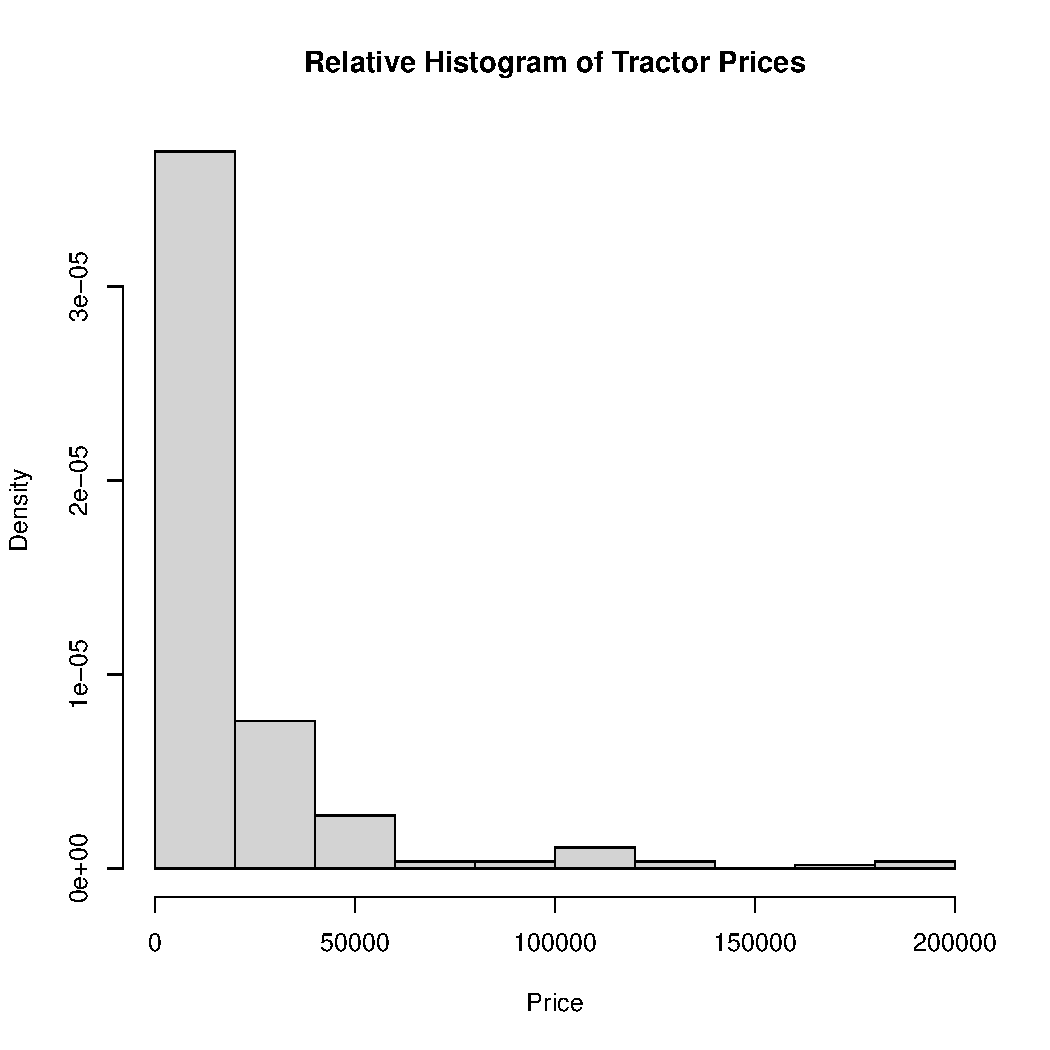
\includegraphics[scale = 0.5, keepaspectratio=true]{../Figures/hist_saleprice}
  \caption{Relative Histogram of Tractor Prices} \label{fig:hist_saleprice}
\end{figure}
%
%
Notice that there are some very large values.
Consider taking logs to bring outliers closer to the others.

\begin{verbatim}
# Generate a new variable log_saleprice.
tractor_sales[, 'log_saleprice'] <- log(tractor_sales[, 'saleprice'])
\end{verbatim}

Now plot the histogram for log of saleprice,
depicted in Figure \ref{fig:hist_log_saleprice}.

\begin{verbatim}
hist(tractor_sales[, 'log_saleprice'],
     main = 'Histogram of the Logarithm of Tractor Prices',
     xlab = 'Logarithm of Price',
     probability = TRUE)
\end{verbatim}


\begin{figure}[h!]
  \centering
  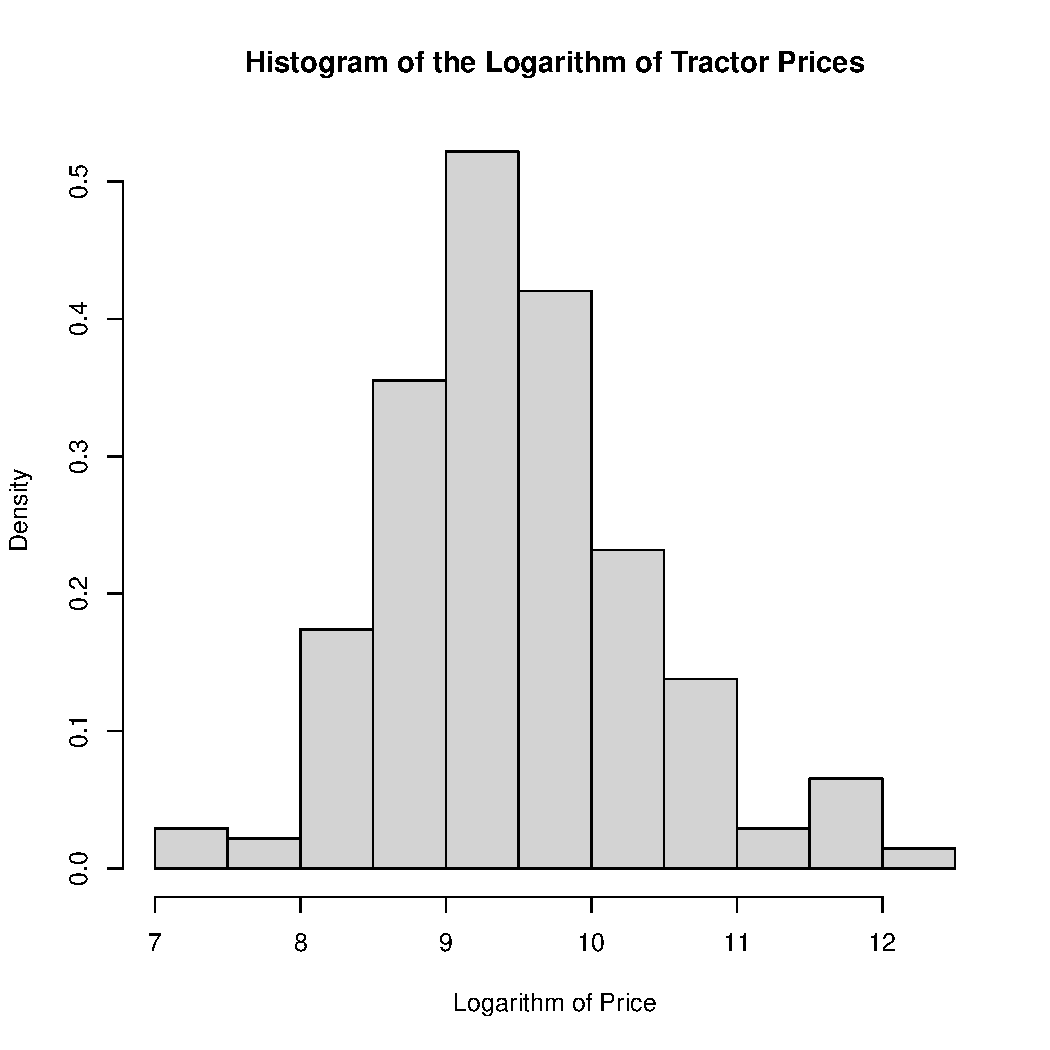
\includegraphics[scale = 0.5, keepaspectratio=true]{../Figures/hist_log_saleprice}
  \caption{Relative Histogram of the Logarithm of Tractor Prices} \label{fig:hist_log_saleprice}
\end{figure}

With this transformation, the variable appears much better behaved.
It looks almost normally distributed.

Now we will consider adjusting the tuning parameter for the number of
bars in the chart for the histogram.
%
A low number of breaks may give a smoother plot but
it may not be very informative, as in Figure \ref{fig:hist_log_saleprice_br5}.

\begin{verbatim}
hist(tractor_sales[, 'log_saleprice'], breaks = 5,
     main = c('Histogram of the Logarithm of Tractor Prices',
              'Number of Breaks: 5'),
     xlab = 'Logarithm of Price',
     probability = TRUE)
\end{verbatim}


\begin{figure}[h!]
  \centering
  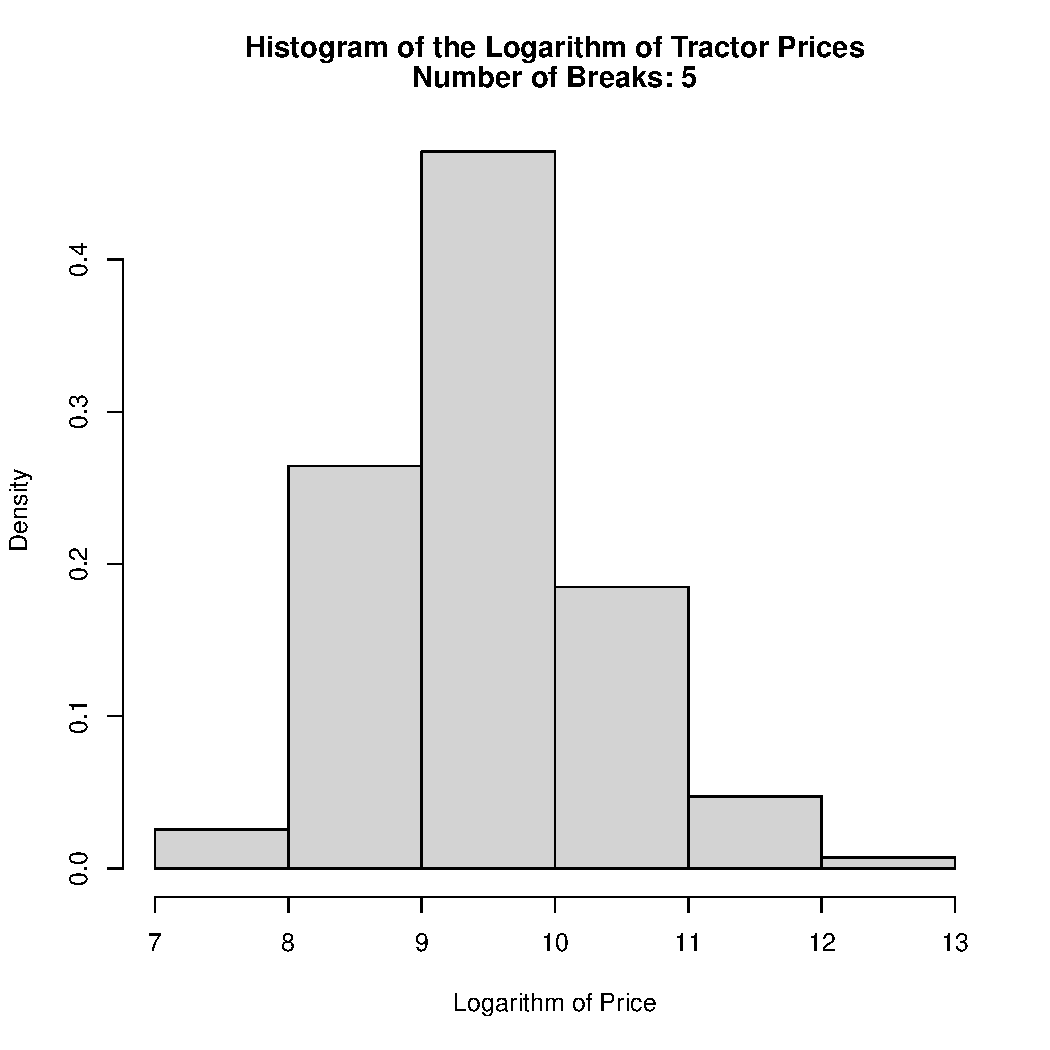
\includegraphics[scale = 0.5, keepaspectratio=true]{../Figures/hist_log_saleprice_br5}
  \caption{Relative Histogram of the Logarithm of Tractor Prices (Breaks: $5$)} \label{fig:hist_log_saleprice_br5}
\end{figure}

On the other extreme,
a high number of breaks gives a sparsely populated
and jagged plot.
Figure \ref{fig:hist_log_saleprice_br50}
shows such an example.

\begin{verbatim}
hist(tractor_sales[, 'log_saleprice'], breaks = 50,
     main = c('Histogram of the Logarithm of Tractor Prices',
              'Number of Breaks: 5'),
     xlab = 'Logarithm of Price',
     probability = TRUE)
\end{verbatim}

\begin{figure}[h!]
  \centering
  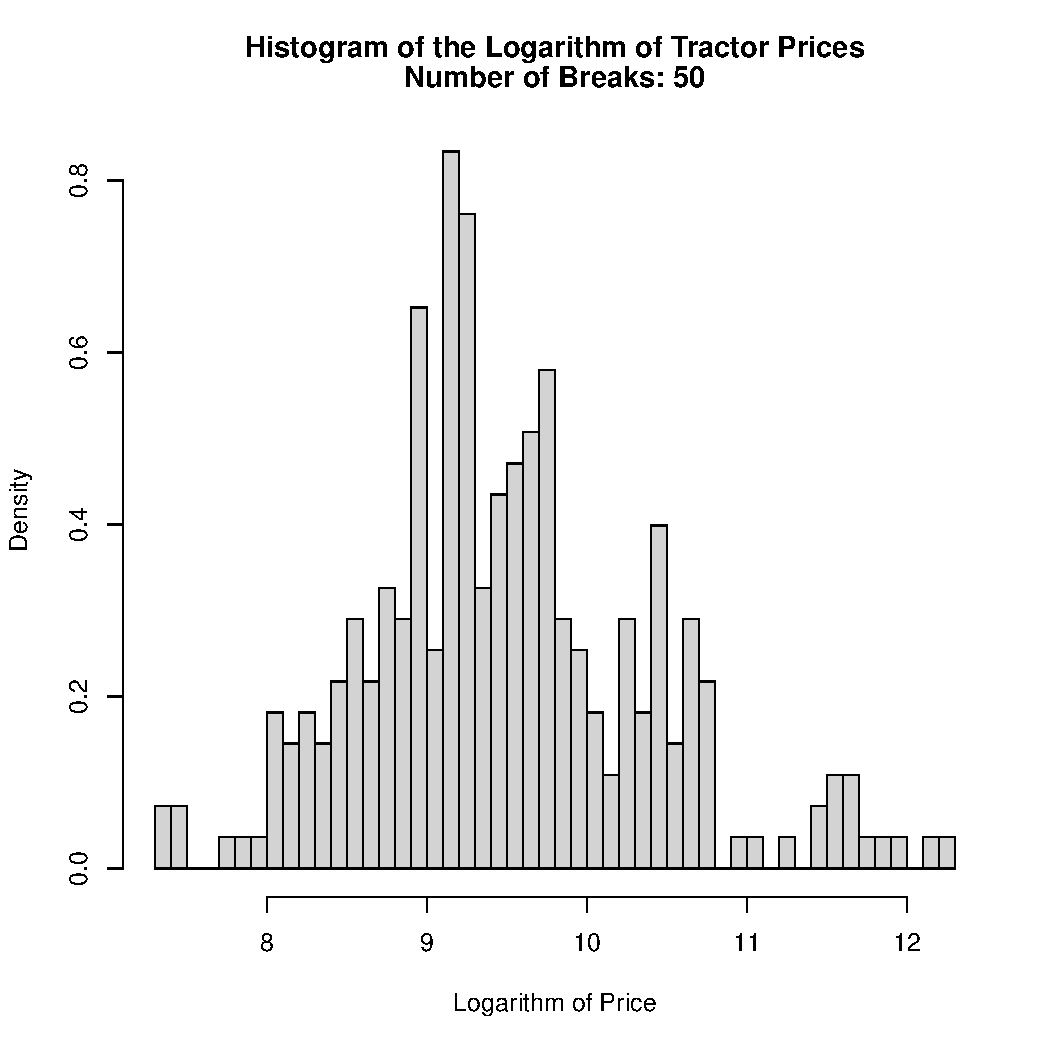
\includegraphics[scale = 0.5, keepaspectratio=true]{../Figures/hist_log_saleprice_br50}
  \caption{Relative Histogram of the Logarithm of Tractor Prices (Breaks: $50$)} \label{fig:hist_log_saleprice_br50}
\end{figure}

\pagebreak
In the limit, the bars can be very small
to the point that each bar is a pixel wide:
approximating a continuous function.
To smooth it out, the nonparametric technique of
kernel smoothing with produce a continuous function.


\pagebreak
\section{Probability Density Function of Tractor Prices}

Kernel-density smoothing is an example of a nonparametric method,
that is, a model without parameters,
such as the slope coefficients $\beta$ in a regression model.
You may have used nonparametric methods to plot a density.
In fact, we have just used a rudimentary form of nonparanetric method
when we plotted the histograms above.


Figure \ref{fig:density_saleprice} depicts
the kernel-smoothed probability density function of the natural logarithm of
price.
\begin{verbatim}
price_density <- density(tractor_sales[, 'saleprice'])
plot(price_density,
     main = 'Kernel-Smoothed Density of Tractor Prices',
     xlab = 'Price')
\end{verbatim}


\begin{figure}[h!]
  \centering
  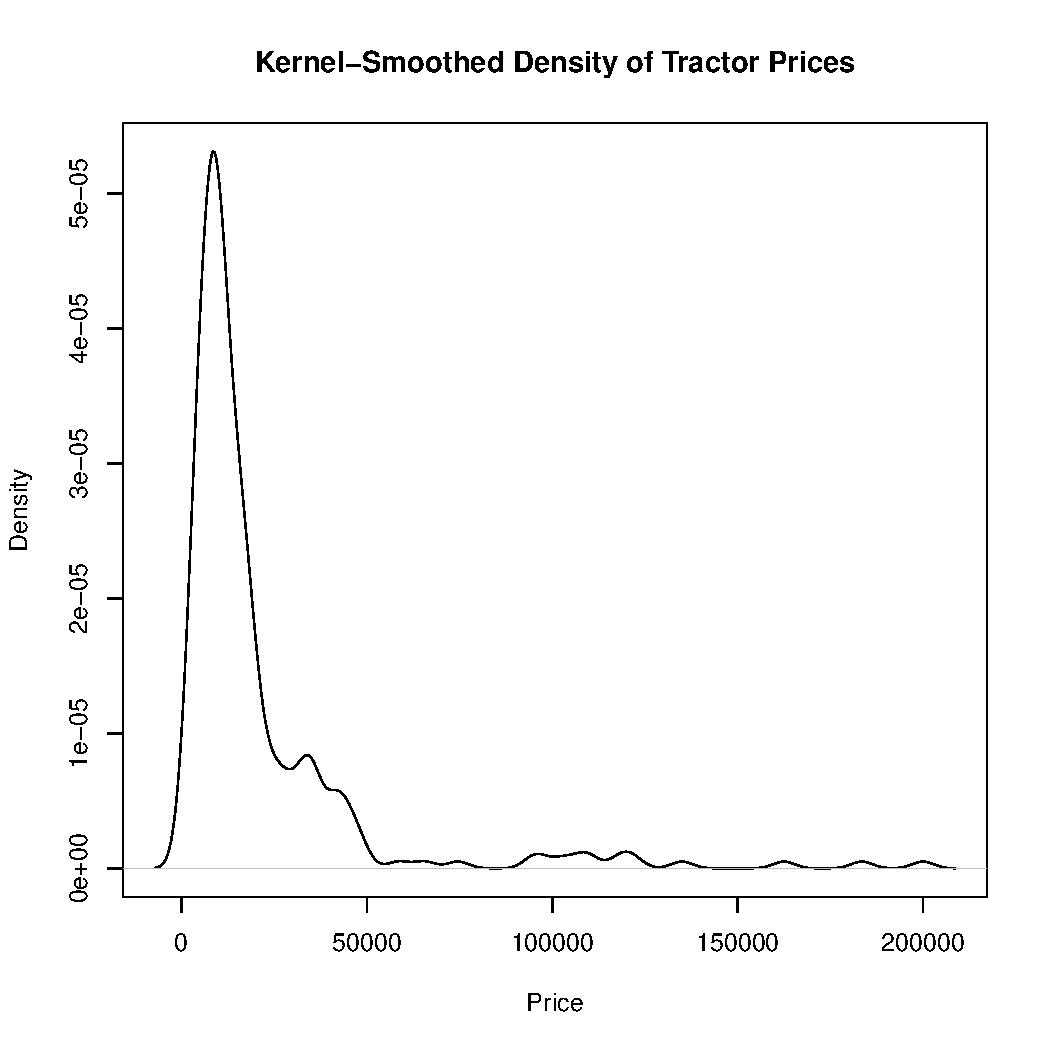
\includegraphics[scale = 0.5, keepaspectratio=true]{../Figures/density_saleprice}
  \caption{Probability Density Function of Tractor Prices} \label{fig:density_saleprice}
\end{figure}

\pagebreak
In the default, the bandwidth is chosen using an algorithm.
See the help for density.

\begin{verbatim}
> attributes(price_density)
$names
[1] "x"         "y"         "bw"        "n"
[5] "call"      "data.name" "has.na"

$class
[1] "density"

> price_density$bw
[1] 2875.455
>
\end{verbatim}

The default algorithm for this variable sets the bandwidth to \$$2,875$.
You can choose the bandwidth as a tuning parameter.
Try a larger value as in the following code block.

\begin{verbatim}
price_density <- density(tractor_sales[, 'saleprice'],
                         bw = 10000)
plot(price_density,
     main = c('Kernel-Smoothed Density of Tractor Prices',
              'Bandwidth: 10,000'),
     xlab = 'Price')
\end{verbatim}

Figure \ref{fig:density_saleprice_bw10000} depicts
the kernel-smoothed probability density function
with a bandwidth of $10,000$.


\begin{figure}[h!]
  \centering
  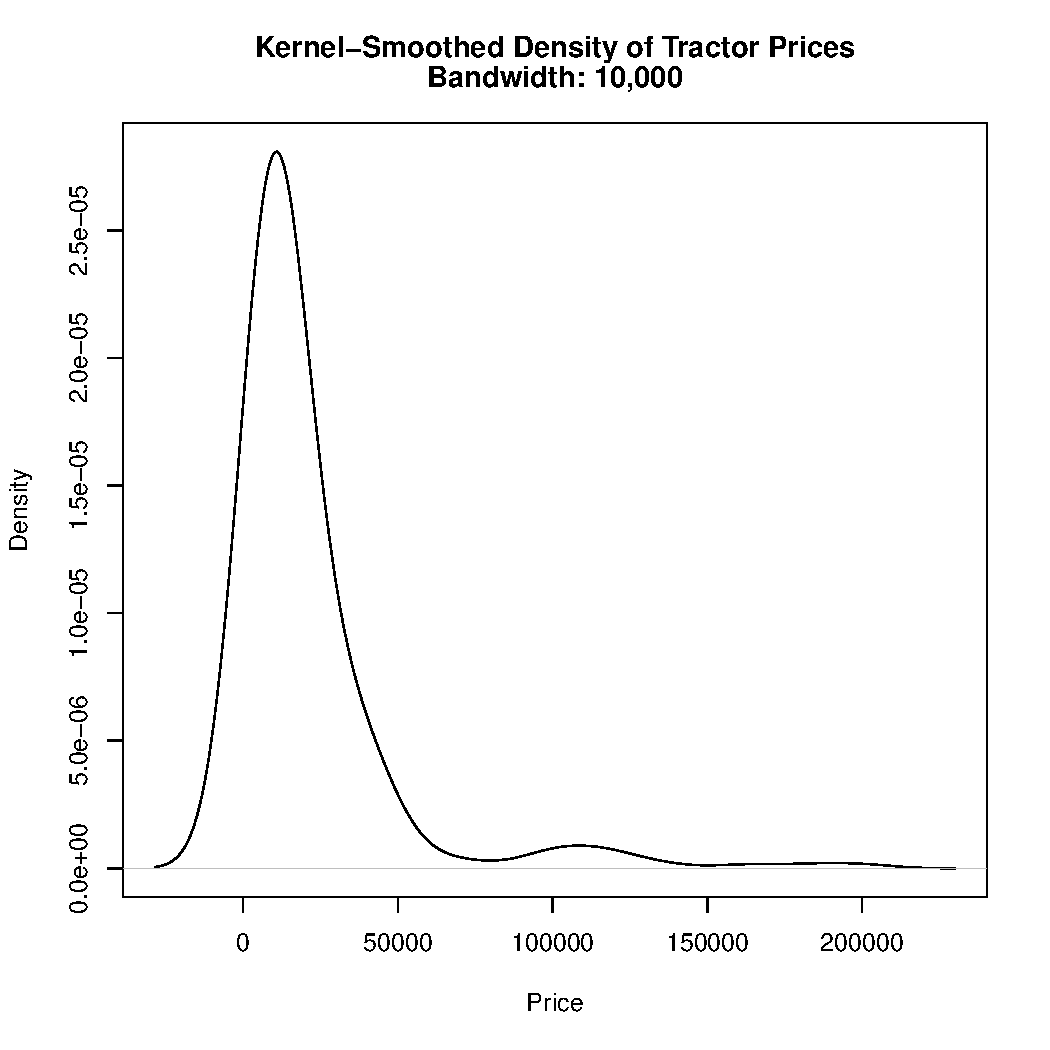
\includegraphics[scale = 0.5, keepaspectratio=true]{../Figures/density_saleprice_bw10000}
  \caption{Probability Density Function of Tractor Prices (Bandwidth: $10,000$)} \label{fig:density_saleprice_bw10000}
\end{figure}

\pagebreak
A bigger bandwidth gives you a smooth density,
but might smooth over the details.
A smaller bandwidth might make the density too noisy.


\begin{verbatim}
price_density <- density(tractor_sales[, 'saleprice'],
                         bw = 1000)
plot(price_density,
     main = c('Kernel-Smoothed Density of Tractor Prices',
              'Bandwidth: 1,000'),
     xlab = 'Price')
\end{verbatim}


\begin{figure}[h!]
  \centering
  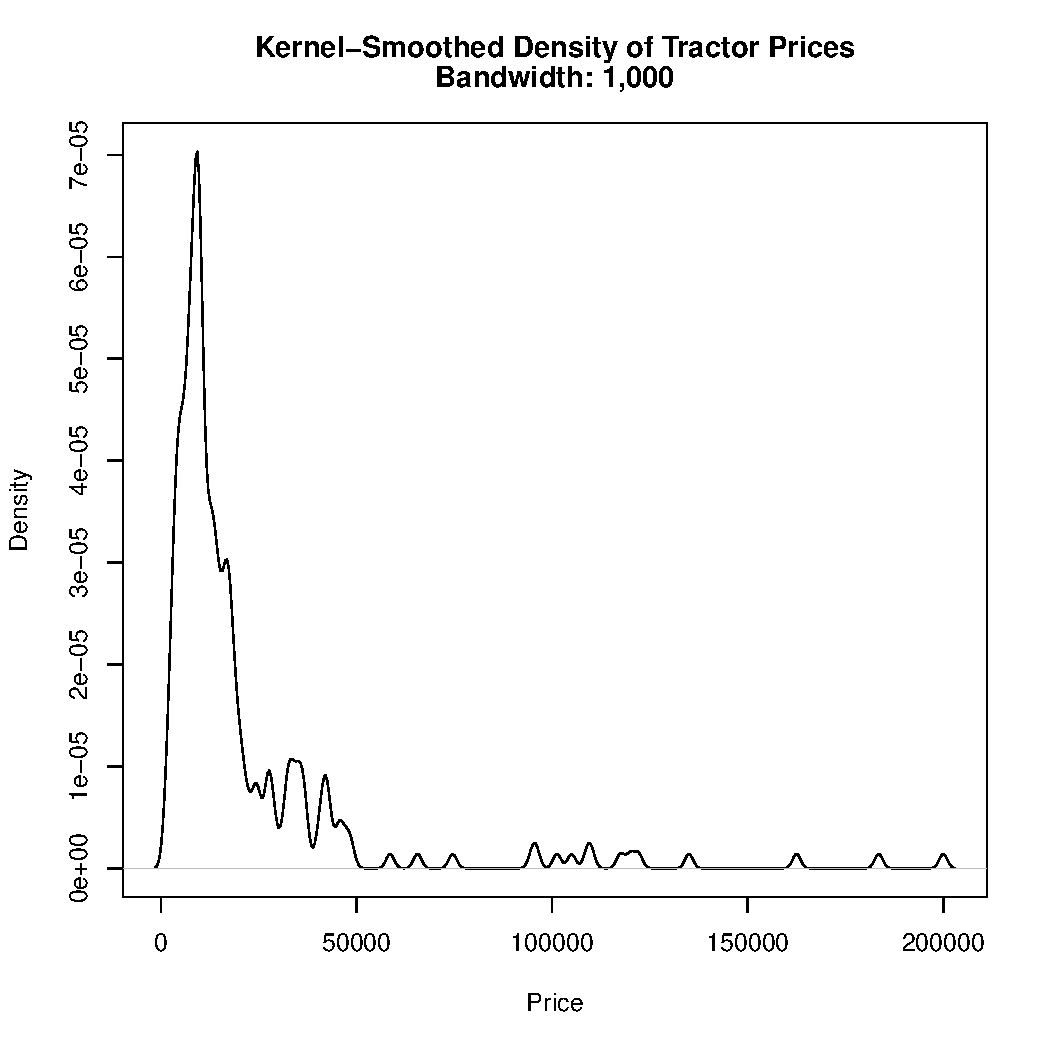
\includegraphics[scale = 0.5, keepaspectratio=true]{../Figures/density_saleprice_bw1000}
  \caption{Probability Density Function of Tractor Prices (Bandwidth: $10,00$)} \label{fig:density_saleprice_bw1000}
\end{figure}

In Figure \ref{fig:density_saleprice_bw1000},
we see many jagged changes that are more closely related
with the particular values observed
than with the population density.

\pagebreak
We can do something similar to predict one variable
with the others.
Before that, we will transform the dependent variable,
after analyzing it in greater detail in future problem sets.
For now, we can plot the logarithm of the dependent variable,
with a bandwidth of $0.20$, which is appropriate for the price levels on a log scale..


\begin{verbatim}
log_price_density <- density(tractor_sales[, 'log_saleprice'],
                         bw = 0.20)
plot(log_price_density,
     main = c('Density of the Logarithm of Tractor Prices',
              'Bandwidth: 0.20'),
     xlab = 'Logarithm of Price')
\end{verbatim}

\begin{figure}[h!]
  \centering
  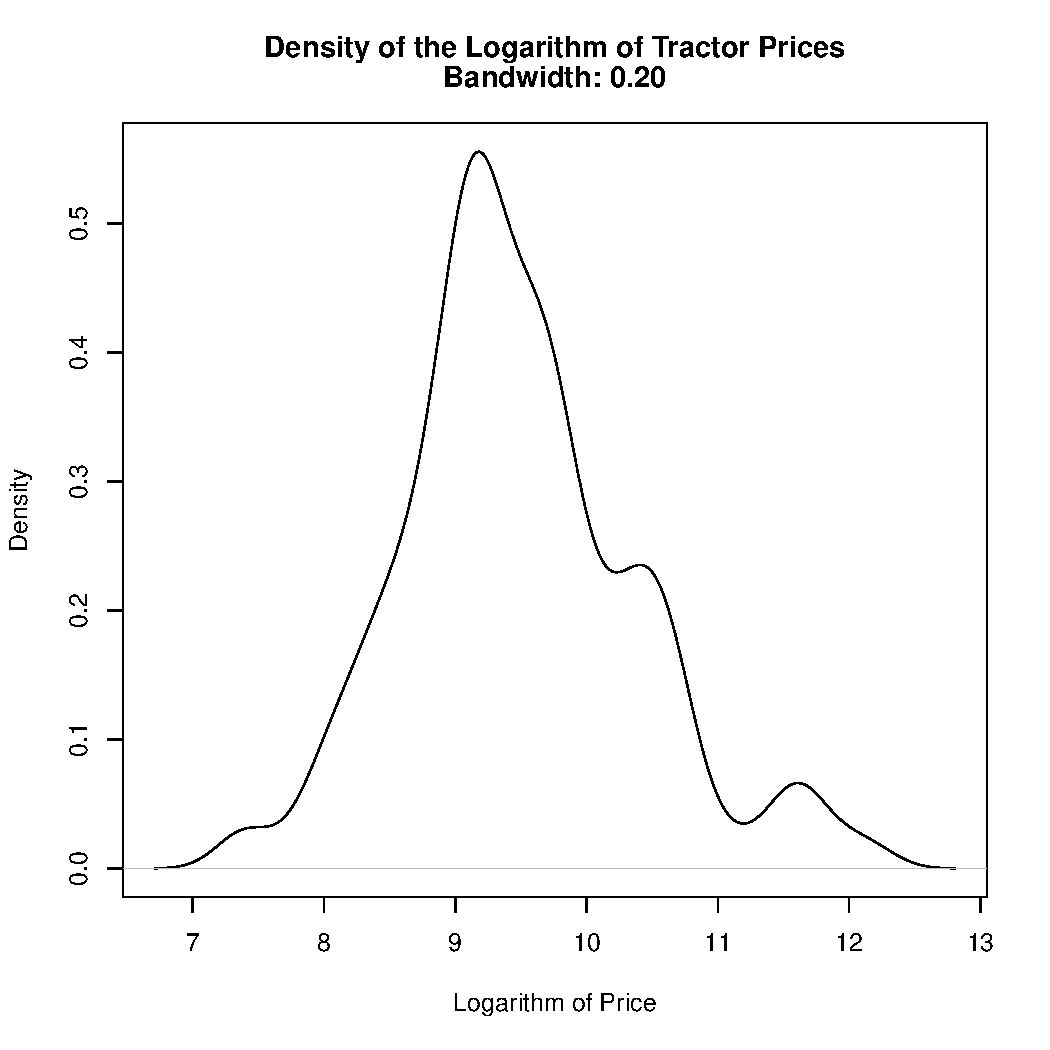
\includegraphics[scale = 0.5, keepaspectratio=true]{../Figures/density_log_saleprice_bw020}
  \caption{Probability Density Function of the Logarithm of Tractor Prices (Bandwidth: $0.20$)} \label{fig:density_log_saleprice_bw020}
\end{figure}


The density plot
shown in Figure \ref{fig:density_log_saleprice_bw020}
is much better behaved and is a good starting point to
analyze the data in a regression model.



%%%%%%%%%%%%%%%%%%%%%%%%%%%%%%%%%%%%%%%%
% \end{document}
%%%%%%%%%%%%%%%%%%%%%%%%%%%%%%%%%%%%%%%%


\pagebreak
\documentclass[11pt]{book}
\usepackage{palatino}
\usepackage{amsfonts,amsmath,amssymb}
% \usepackage{graphicx}

\usepackage{listings}
\usepackage{textcomp}
\usepackage{color}

\definecolor{dkgreen}{rgb}{0,0.6,0}
\definecolor{gray}{rgb}{0.5,0.5,0.5}
\definecolor{mauve}{rgb}{0.58,0,0.82}

\lstset{frame=tb,
  language=R,
  aboveskip=3mm,
  belowskip=3mm,
  showstringspaces=false,
  columns=flexible,
  basicstyle={\small\ttfamily},
  numbers=none,
  numberstyle=\tiny\color{gray},
  keywordstyle=\color{blue},
  commentstyle=\color{dkgreen},
  stringstyle=\color{mauve},
  breaklines=true,
  breakatwhitespace=true,
  tabsize=3
}



\ifx\pdftexversion\undefined
    \usepackage[dvips]{graphicx}
\else
    \usepackage[pdftex]{graphicx}
    \usepackage{epstopdf}
    \epstopdfsetup{suffix=}
\fi

\usepackage{subfig}

\begin{document}

%%%%%%%%%%%%%%%%%%%%%%%%%%%%%%%%%%%%%%%%
% Problem Set 6
%%%%%%%%%%%%%%%%%%%%%%%%%%%%%%%%%%%%%%%%

\pagestyle{empty}
{\noindent\bf Spring 2021 \hfill Firstname M.~Lastname}
\vskip 16pt
\centerline{\bf University of Central Florida}
\centerline{\bf College of Business}
\vskip 16pt
\centerline{\bf QMB 6911}
\centerline{\bf Capstone Project in Business Analytics}
\vskip 10pt
\centerline{\bf Solutions:  Problem Set \#6}
\vskip 32pt
\noindent


%%%%%%%%%%%%%%%%%%%%%%%%%%%%%%%%%%%%%%%%
% Density Plots and Q-Q Plots
%%%%%%%%%%%%%%%%%%%%%%%%%%%%%%%%%%%%%%%%


\pagebreak
\section*{Probability Density Function of Tractor Prices}

Figure \ref{fig:density_prices} shows  the kernel-smoothed probability density function of tractor prices.

\begin{figure}[h!]
  \centering
  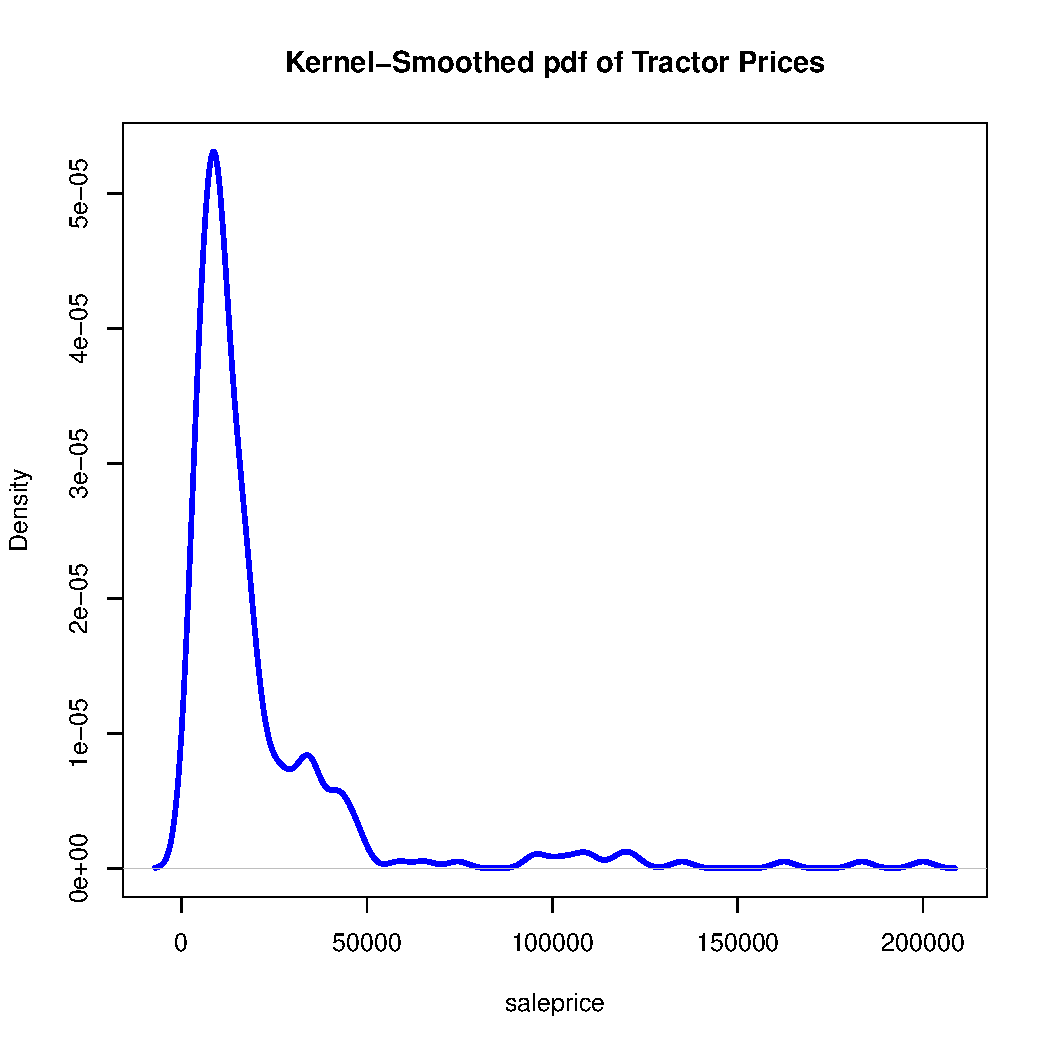
\includegraphics[scale = 0.5, keepaspectratio=true]{../Figures/density_prices}
  \caption{Probability Density Function of Tractor Prices} \label{fig:density_prices}
\end{figure}



\pagebreak
As a comparison, Figure \ref{fig:density_log_prices} shows the kernel-smoothed probability density function of the natural logarithm of
price.

\begin{figure}[h!]
  \centering
  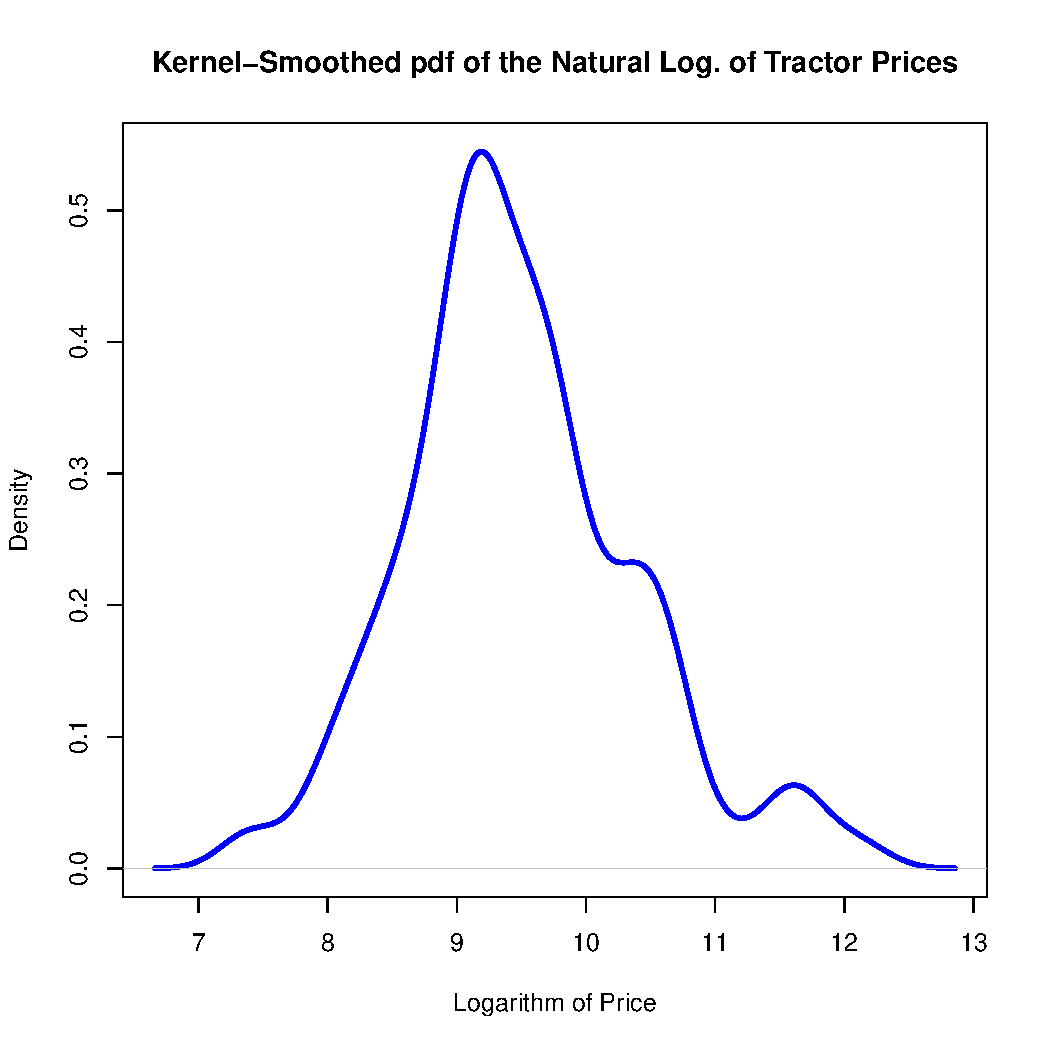
\includegraphics[scale = 0.5, keepaspectratio=true]{../Figures/density_log_prices}
  \caption{Probability Density Function of the Logarithm of Tractor Prices} \label{fig:density_log_prices}
\end{figure}




\pagebreak
\section*{Normality of the Original and Transformed Variables}

Figure \ref{fig:qq_prices} shows a pair of Q-Q plots, 
comparing quantiles of the empirical distribution against
the quantiles of the normal distribution. 
In the left panel, Figure \ref{subfig:qq_prices} shows this comparison 
for the original level of the tractor prices, without transformation. 
In the right panel, Figure \ref{subfig:qq_log_prices} shows this comparison 
for the logarithmic transformation of tractor prices, without transformation. 
Consistent with the pair of distributions estimated above, 
each plot shows a divergence from a normal distribution,
suggesting that an optimal transformation might lie somewhere else.
The Box-Cox transformation allows for this possibility. 

\begin{figure}[!ht]
\subfloat[Tractor Prices\label{subfig:qq_prices}]{%
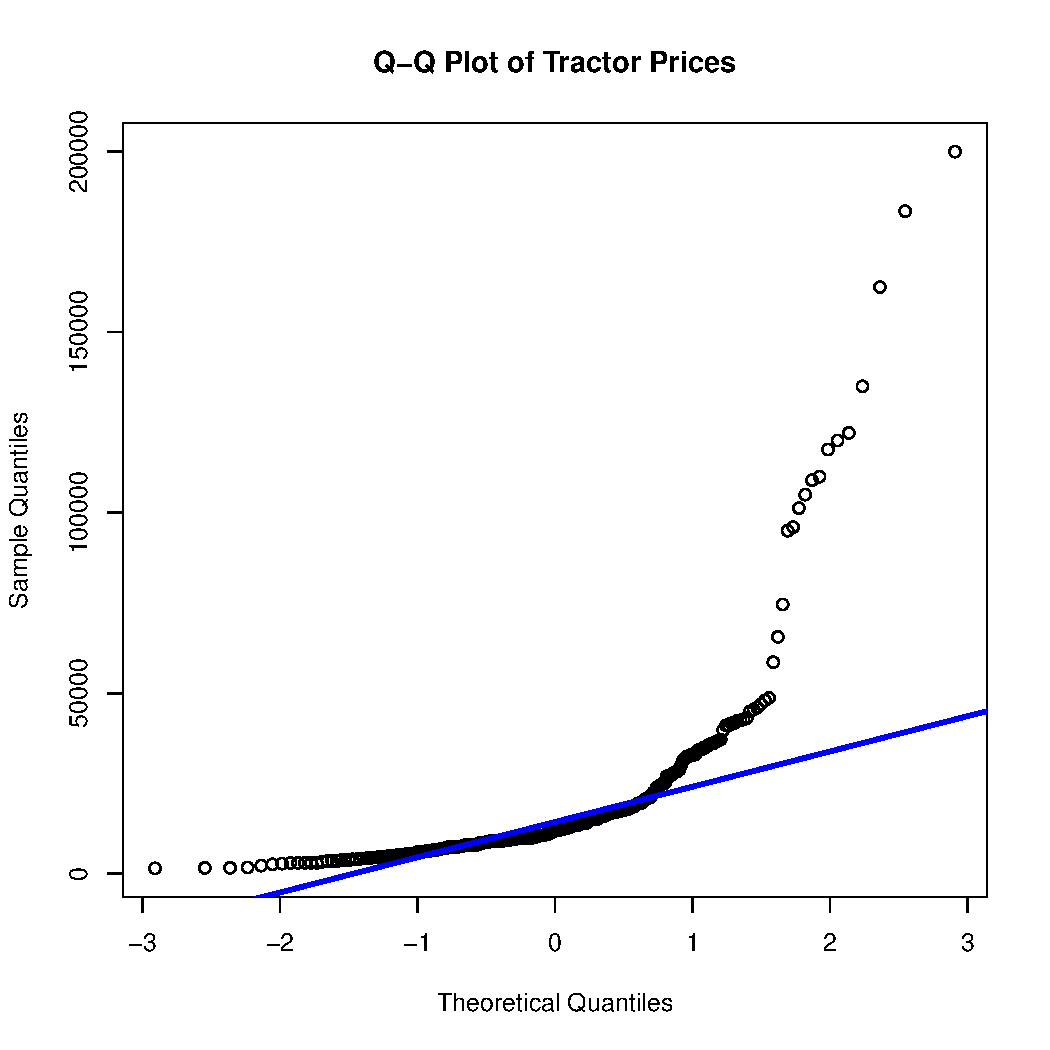
\includegraphics[width=0.5\textwidth]{../Figures/qq_prices}}
\hfill
\subfloat[Transformed Tractor Prices\label{subfig:qq_log_prices}]{%
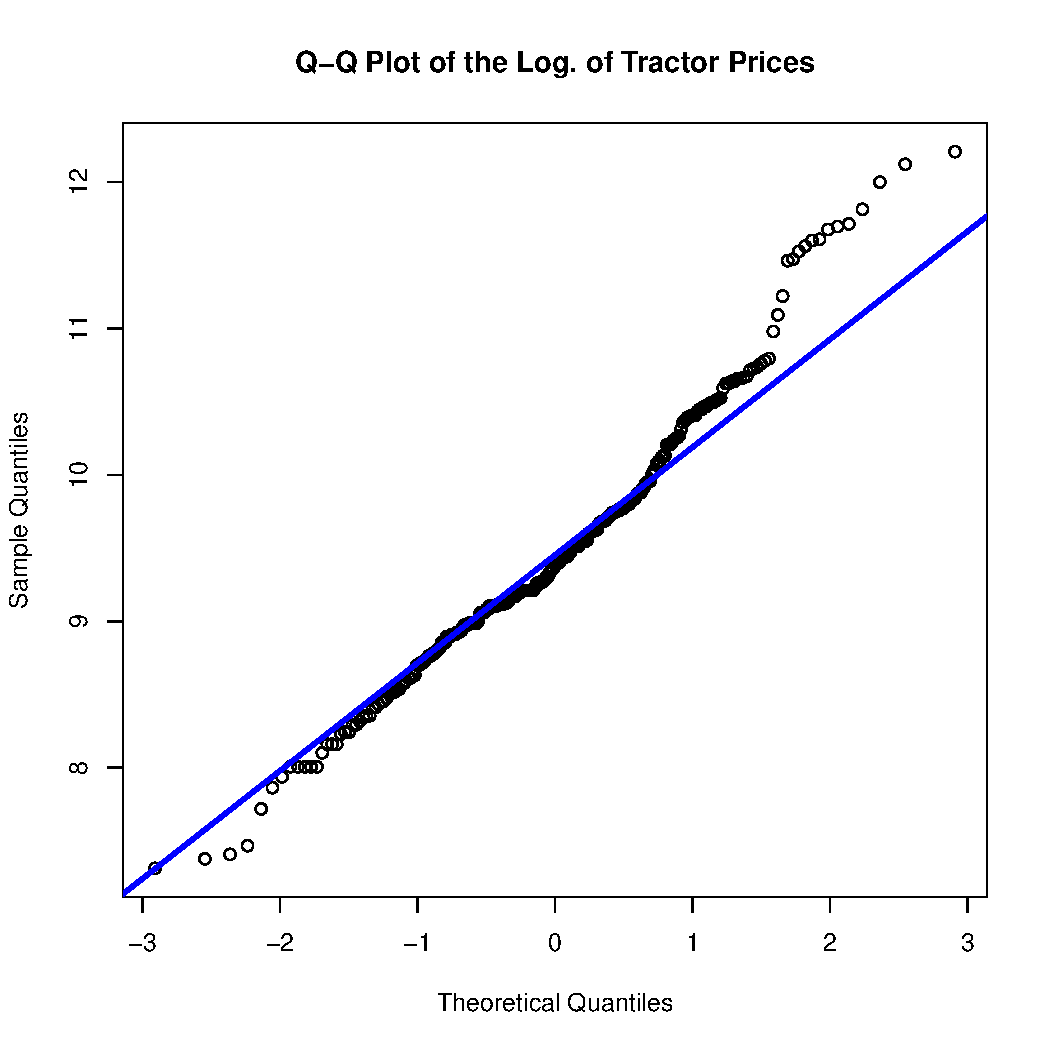
\includegraphics[width=0.5\textwidth]{../Figures/qq_log_prices}}

\caption{Q-QPlots of the Log. and Levels of Tractor Prices}
\label{fig:qq_prices}
\end{figure}



%%%%%%%%%%%%%%%%%%%%%%%%%%%%%%%%%%%%%%%%
% Box-Cox Transformation
%%%%%%%%%%%%%%%%%%%%%%%%%%%%%%%%%%%%%%%%


\pagebreak
\section{Box-Cox Transformation of Tractor Prices}

Under the Box--Cox transformation of $P_n$, the price of tractor $n$
is calculated as follows,
$$\Lambda(P_n)\equiv
  \begin{cases}
	\frac{P_n^\lambda-1}{\lambda}	& \textrm{if } \lambda > 0 \\
           \log P_n                     			& \textrm{if } \lambda = 0.\\
  \end{cases}
$$
The following code block defines a function that performs a
Box-Cox transformation.

\vspace{1.0in}

\begin{lstlisting}[language=R]
# Box-Cox transformation.
Lambda_Price <- function(price, lambda) {
  if (lambda == 0) {
    return(log(price))
  } else {
    return((price^lambda - 1)/lambda)
  }
}
\end{lstlisting}

\pagebreak
\subsection{Log-likelihood Function}

Under the Box-Cox transformation,
the tractor prices can be decomposed into a location parameter $\mu^0$ 
and an error $U$, so
$$\Lambda(P_n) = \mu^0(\lambda) + U_n,$$
where the $U_n$s are independent, mean-zero, constant-variance 
$\sigma^2(\lambda)$, Gaussian (normal) errors. 
In the above equation, for clarity, the dependence of $\mu^0$ and 
$\sigma^2(\lambda)$ on $\lambda$ is made explicit.


The next code block defines a likelihood function for the normal distribution of the errors
as a function of the parameter $\lambda$.

\begin{lstlisting}[language=R]
log_like_uni <- function(price, lambda) {

  # Calculate maximum likelighood estimates of the parameters.
  n <- length(price)
  lambda_price <- Lambda_Price(price, lambda)
  mu_0_lambda <- mean(lambda_price)
  sigma_2_lambda <- sum((lambda_price - mu_0_lambda)^2)/n

  # Calculate the log-likelihood from the sum of the logarithms
  # of the density of the normal distribution.
  like <- - n/2*log(2*pi*sigma_2_lambda)
  like <- like - 1/2/sigma_2_lambda*sum((lambda_price - mu_0_lambda)^2)
  like <- like + (lambda - 1)*sum(log(price))
  return(like)
}
\end{lstlisting}

\pagebreak
As a first approximation, 
One can calculate the value of the log-likelihood function on a grid of values
to find an optimal value of $\lambda$.
The plot of this likelihood function is shown in Figure \ref{fig:box_cox_loglike_uni}.
The red points represent the values of the log-likelihood 
at the optimum $\lambda = -0.17$ and at $\lambda = 0$ and $\lambda = 1$.

\begin{lstlisting}[language=R]
# Calculate values of the log-likelihood function.
lambda_grid <- seq(-1, 2.5, by = 0.001)
like_grid <- 0*lambda_grid
for (lambda_num in 1:length(lambda_grid)) {
  like_grid[lambda_num] <- log_like_uni(price = tractor_sales[, 'saleprice'],
                                    lambda = lambda_grid[lambda_num])
}
\end{lstlisting}

\begin{figure}[h!]
  \centering
  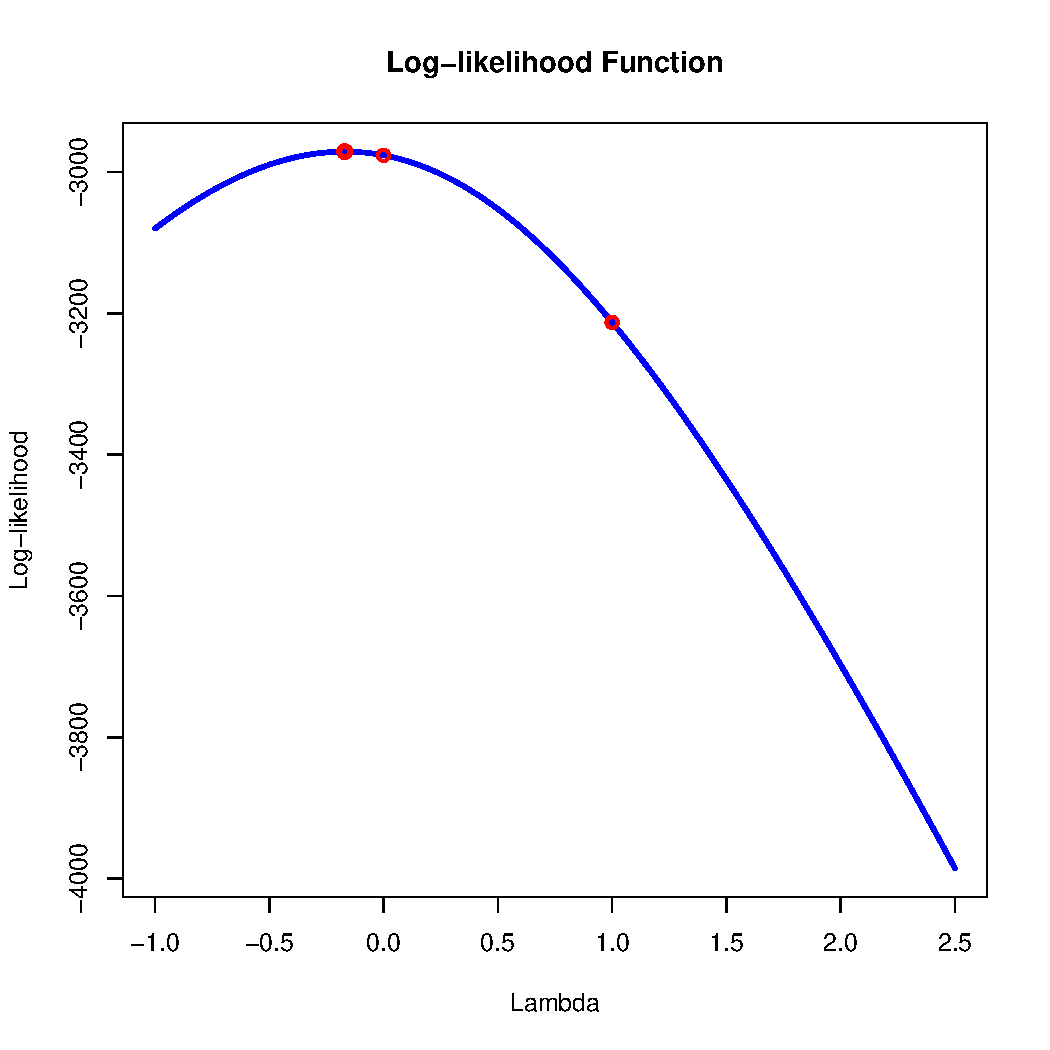
\includegraphics[scale = 0.5, keepaspectratio=true]{../Figures/box_cox_loglike_uni}
  \caption{Log-likelihood Function for Box-Cox Transformation} \label{fig:box_cox_loglike_uni}
\end{figure}


\pagebreak
\subsection{Testing for an Appropriate Transformation}

Now we consider the statistical properties of these estimates
by calculating a likelihood ratio statistic.

\begin{lstlisting}[language=R]
> # Calculate likelihood ratio statistics.
> LR_stat_0 <- - 2*(like_mu_0 - like_MLE)
> print(LR_stat_0)
[1] 10.26956
> LR_stat_1 <- - 2*(like_mu_1 - like_MLE)
> print(LR_stat_1)
[1] 483.2539
> 
> 
> # Compare to quantile of chi-squared distribution with 1 degree of freedom.
> LR_cv_5 <- qchisq(p = 0.95, df = 1)
> print(LR_cv_5)
[1] 3.841459
> 
> # Calculate p-values for these tests.
> p_value_0 <- 1 - pchisq(q = LR_stat_0, df = 1)
> print(p_value_0)
[1] 0.001352434
> p_value_1 <- 1 - pchisq(q = LR_stat_1, df = 1)
> print(p_value_1)
[1] 0
> 
\end{lstlisting}

Statistically, this is evidence to reject them both.
This suggests using the transformation at the MLE.
However, one may want to investigate further 
to find out whether it is worth 
transforming the data, 
since the Box-Cox transformation at the MLE offers only a marginal improvement over the log transformation. 
There exists a trade-of between interpretability and 
the accuracy of the statistical specification, 
and, perhaps, the log transformation is close enough 
for practical purposes. 


\clearpage
\section{\textsf{R} Packages for the Box-Cox Transformation}
\subsection*{Using the \texttt{MASS} Package}

As an illustration, we calculated
the likelihood ourselves.
However, there exist other packages
to output the estimation results for
an optimal Box-Cox transformation.

One option is to use the function from the \texttt{MASS} package.
This is an \textsf{R} package that accompanies a well-know statistics textbook
and has a great reputation. 
In the \texttt{MASS} package, the notation is the same as for a linear model.


\begin{lstlisting}[language=R]
# In the MASS package, the notation is the same as for a linear model.
# i.e., summary(lm(saleprice ~ 1, data = tractor_sales))
bc_grid_MASS <- MASS::boxcox(saleprice ~ 1,
                             data = tractor_sales,
                             lambda = lambda_grid)
\end{lstlisting}

The output is plotted in Figure \ref{fig:plot_like_MASS}.

\begin{figure}[h!]
  \centering
  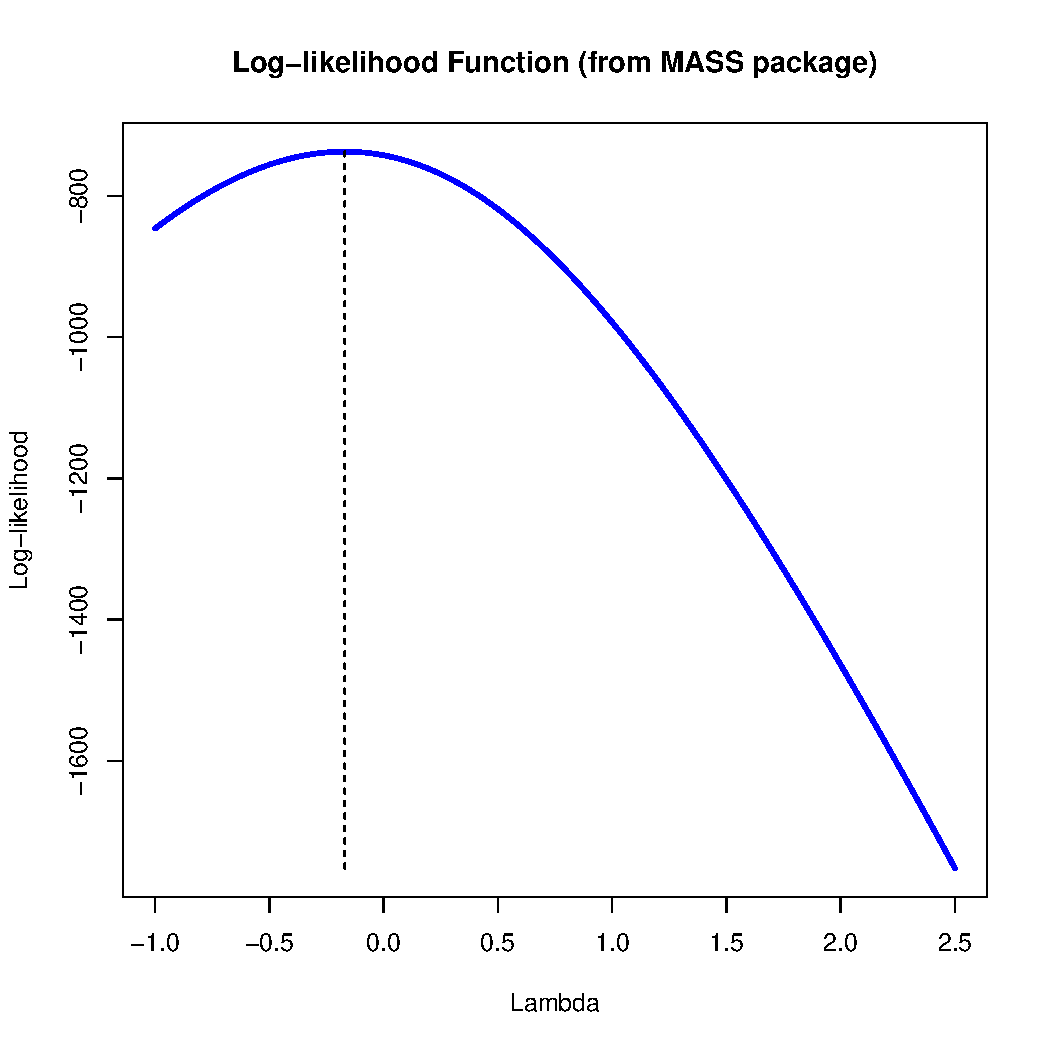
\includegraphics[scale = 0.5, keepaspectratio=true]{../Figures/plot_like_MASS}
  \caption{Log-likelihood Function for Box-Cox Transformation (\texttt{MASS} package)} \label{fig:plot_like_MASS}
\end{figure}


\clearpage
\section*{Using the \texttt{car} Package}

The \texttt{car} package is another well-known option.
With this function, the optimization produces 
a figure automatically from the code below.

\begin{lstlisting}[language=R]
bc_grid_car <- car::boxCox(object = lm(data = tractor_sales,
                                       formula = saleprice ~ 1),
                           lambda = lambda_grid)
\end{lstlisting}

The output is plotted in Figure \ref{fig:plot_like_car}.

\begin{figure}[h!]
  \centering
  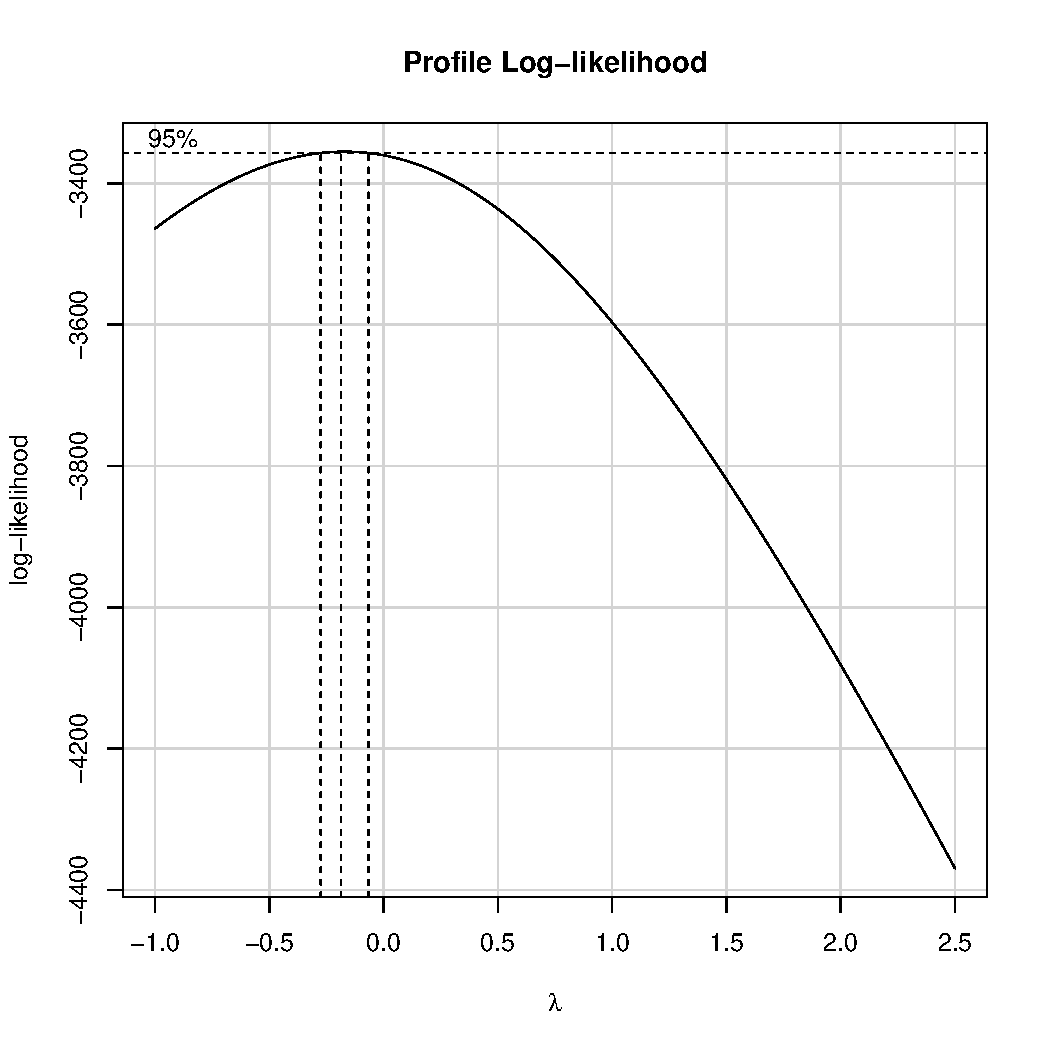
\includegraphics[scale = 0.5, keepaspectratio=true]{../Figures/plot_like_car}
  \caption{Log-likelihood Function for Box-Cox Transformation (\texttt{car} package)} \label{fig:plot_like_car}
\end{figure}


\clearpage
\section*{Using the \texttt{EnvStats} Package}


The \texttt{EnvStats} package is another option
but it is one designed for environmental statistics.
That is, it is not a generic package designed for the population of statisticians at large.
For that reason, it is missing some of the features that
a statistician would expect.
The notation and interpretation, however, are similar, 
except that the straight call to \texttt{boxcox}
simply does the calculation, 
unless you specify otherwise.

\begin{lstlisting}[language=R]
> # Find optimal value of lambda.
> bc_grid_ES_opt <- EnvStats::boxcox(x = tractor_sales[, 'saleprice'],
+                                    lambda = range(lambda_grid),
+                                    optimize = TRUE,
+                                    objective.name = "Log-Likelihood")
> 
> bc_grid_ES_opt$lambda
[1] 0.4295551
> 
\end{lstlisting}


The output is plotted in Figure \ref{fig:plot_like_EnvStats}.

\begin{figure}[h!]
  \centering
  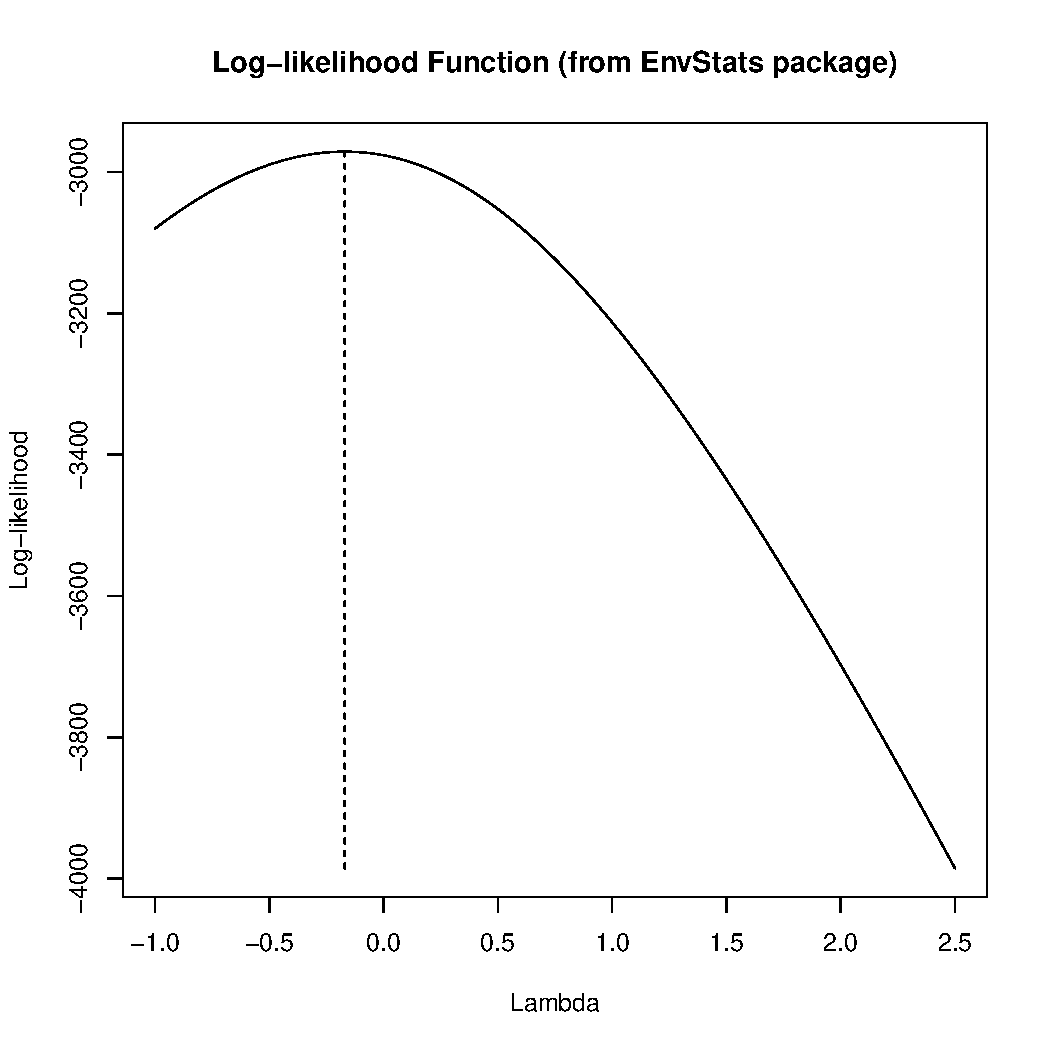
\includegraphics[scale = 0.5, keepaspectratio=true]{../Figures/plot_like_EnvStats}
  \caption{Log-likelihood Function for Box-Cox Transformation (\texttt{EnvStats} package)} \label{fig:plot_like_EnvStats}
\end{figure}






\clearpage
\section*{Normality of the Transformed Variable}

Now compare the quantiles of the distribution of the transformed variable with 
the original. 
We already plotted normal QQ plot for tractor prices when considering the log transformation.
Now we can generate a new dependent variable with the results from the estimates above.


\begin{lstlisting}[language=R]
# Generate new dependent variable with results from estimates above.
tractor_sales[, 'trans_saleprice'] <- Lambda_Price(price = tractor_sales[, 'saleprice'],
                                          lambda = lambda_hat)
\end{lstlisting}

Figure \ref{fig:qq2_prices} shows this comparison
and the panel on the right, Figure \ref{subfig:qq2_boxcox}, 
shows that the quantiles of the distribution of the transformed variable
nearly overlap with those of the normal distribution.
From a purely statistical perspective, 
this provides evidence that the prices are best modeled with the transformation
at the optimal $\lambda = -0.17$.
From a practical point of view, however, 
the added complexity is not warranted
when the log transformation is close enough.


\begin{figure}[!ht]
\subfloat[Log. of Tractor Prices\label{subfig:qq_log2_prices}]{%
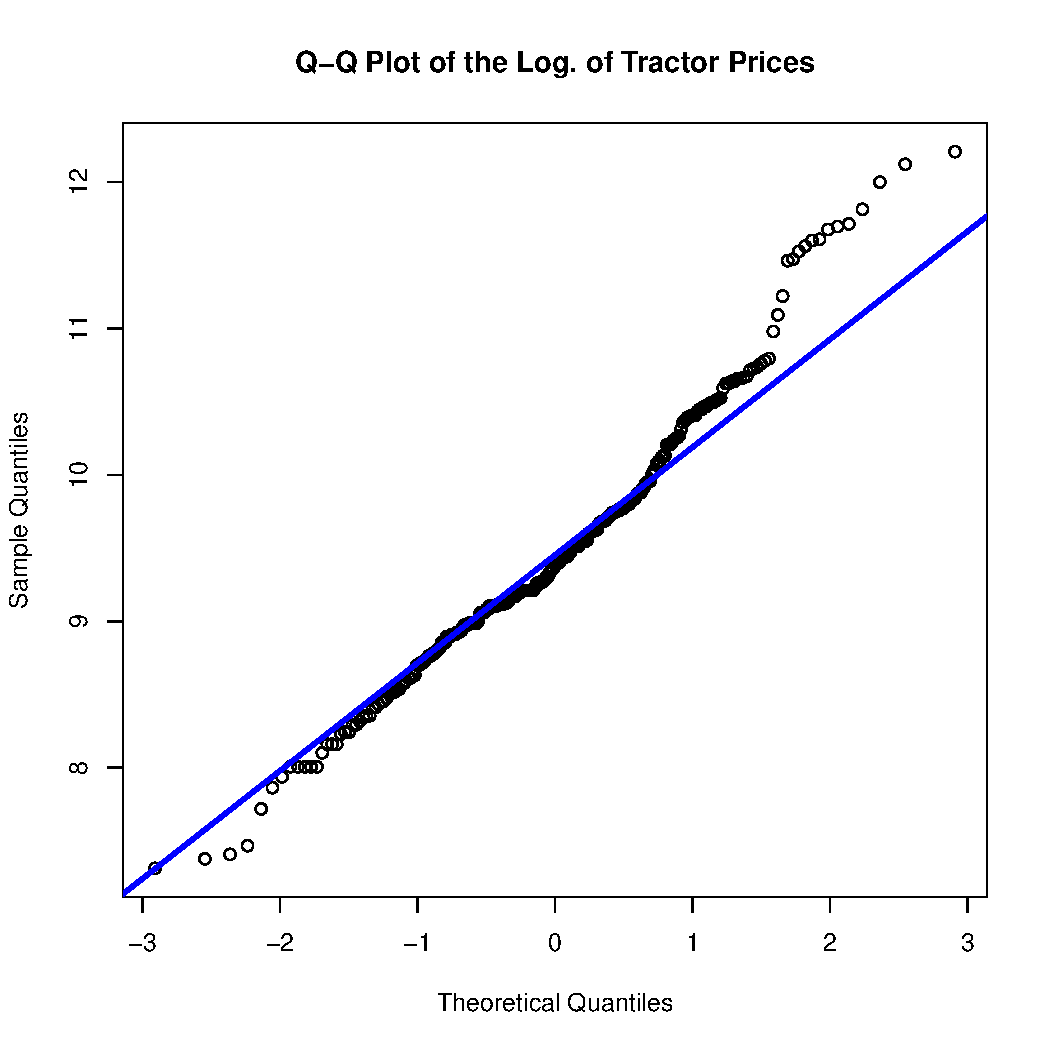
\includegraphics[width=0.5\textwidth]{../Figures/qq_log_prices}}
\hfill
\subfloat[Transformed Tractor Prices\label{subfig:qq2_boxcox}]{%
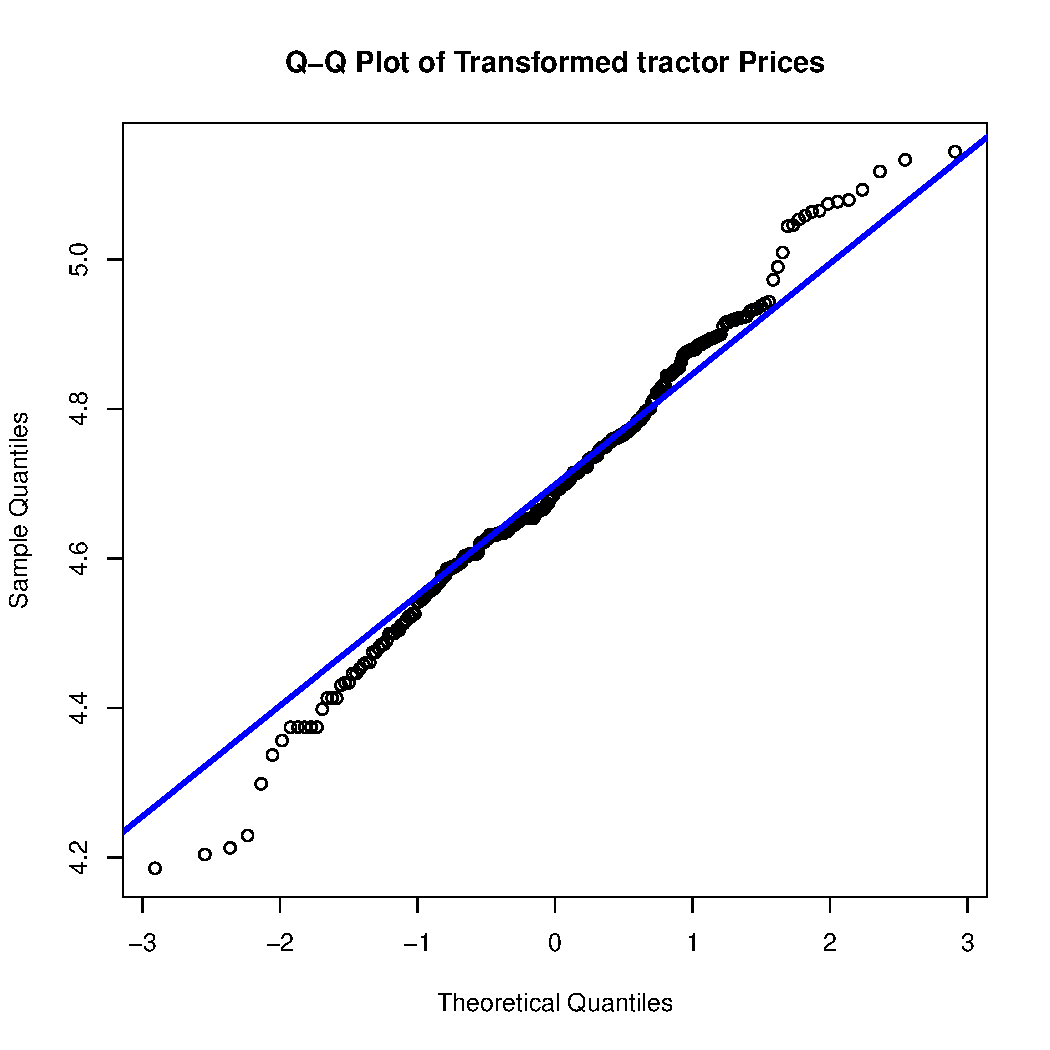
\includegraphics[width=0.5\textwidth]{../Figures/qq_boxcox}}

\caption{Q-QPlots of the Transformed Tractor Prices}
\label{fig:qq2_prices}
\end{figure}








%%%%%%%%%%%%%%%%%%%%%%%%%%%%%%%%%%%%%%%%
\end{document}
%%%%%%%%%%%%%%%%%%%%%%%%%%%%%%%%%%%%%%%%


\pagebreak
\input{Tractor_Tables}

\pagebreak
\documentclass[11pt]{book}
\usepackage{palatino}
\usepackage{amsfonts,amsmath,amssymb}

% Packages for Figures:
% Without conversion of eps to pdf:
\usepackage{graphicx}
% With conversion of eps to pdf,
% which depends on platform.
%\ifx\pdftexversion\undefined
%    \usepackage[dvips]{graphicx}
%\else
%    \usepackage[pdftex]{graphicx}
%    \usepackage{epstopdf}
%    \epstopdfsetup{suffix=}
%\fi

% Packages for displaying code:
\usepackage{listings}
\usepackage{textcomp}
\usepackage{color}

% Color settings used in the code below:
\definecolor{dkgreen}{rgb}{0,0.6,0}
\definecolor{gray}{rgb}{0.5,0.5,0.5}
\definecolor{mauve}{rgb}{0.58,0,0.82}

% Settings for the formatting of the code on display:
\lstset{frame=tb,
  language=R,
  aboveskip=3mm,
  belowskip=3mm,
  showstringspaces=false,
  columns=flexible,
  basicstyle={\small\ttfamily},
  numbers=none,
  numberstyle=\tiny\color{gray},
  keywordstyle=\color{blue},
  commentstyle=\color{dkgreen},
  stringstyle=\color{mauve},
  breaklines=true,
  breakatwhitespace=true,
  tabsize=3
}

% Package for displaying inline verbatim commands in footnotes.
\usepackage{fancyvrb}


\begin{document}

%%%%%%%%%%%%%%%%%%%%%%%%%%%%%%%%%%%%%%%%
% Problem Set 4
%%%%%%%%%%%%%%%%%%%%%%%%%%%%%%%%%%%%%%%%

\pagestyle{empty}
{\noindent\bf Spring 2021 \hfill Firstname M.~Lastname}
\vskip 16pt
\centerline{\bf University of Central Florida}
\centerline{\bf College of Business}
\vskip 16pt
\centerline{\bf QMB 6911}
\centerline{\bf Capstone Project in Business Analytics}
\vskip 10pt
\centerline{\bf Solutions:  Problem Set \#5}
\vskip 32pt
\noindent

\section{Introduction}

This note summarizes the findings in the script
\texttt{Tractor\_Data\_Vis.R},
which analyzes the prices of used tractors,
the dependent variable in the \texttt{TRACTOR7.csv} dataset.
The output includes several plots of the
dependent variable against the explanatory variables.

The primary goal is to determine the relative value of John Deere tractors compared to others.
A secondary consideration is to determine the time of year in which to
sell a tractor.

\vfill
\pagebreak
\section{Histogram and Density of Log. Tractor Prices}


\subsection{All Tractors Together}

Start with the log of sale prices because that
seemed more promising, given that prices were highly skewed.

\begin{lstlisting}[language=R]
hist(tractor_sales[, 'log_saleprice'],
     main = 'Histogram and Density of Log. Tractor Prices',
     xlab = 'Price', col = 'red',
     probability = TRUE)
rug(tractor_sales[, 'log_saleprice'])
lines(density(tractor_sales[, 'log_saleprice']),
      col = 'blue', lwd = 3)
\end{lstlisting}


Figure \ref{fig:hist_dens_log_price} is
a histogram of the logarithm of tractor prices,
along with a rug plot and a kernel density estimate,
generated by the code block above.
%
\begin{figure}[h!]
  \centering
  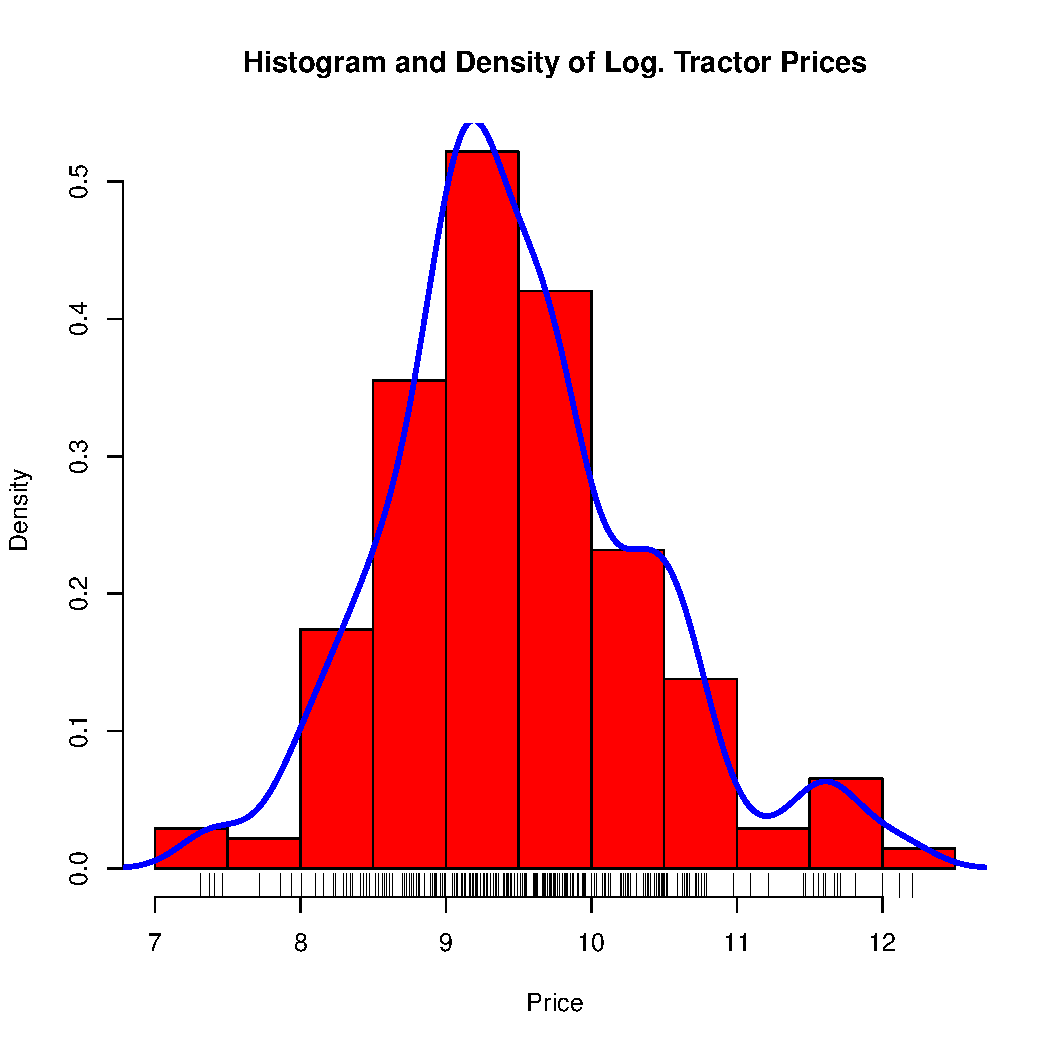
\includegraphics[scale = 0.5, keepaspectratio=true]{../Figures/hist_dens_log_price}
  \caption{Relative Histogram of Tractor Prices} \label{fig:hist_dens_log_price}
\end{figure}
%
After taking logs, we can see that the distribution is
approximately symmetric, with some bunching in the
upper tail.

\pagebreak
\subsection{Comparison By Make}

Now we investigate the value of John Deere tractors
compared to other brands.
Figure \ref{fig:dens_by_brand} shows the
kernel density estimate of the sale prices of John Deere tractors
in green and that of the other brands in red.
%
The distribution of sale prices of John Deere tractors has several modes and is skewed to the right,
with the highest mode lower than that for other brands.


\begin{lstlisting}[language=R]
library(sm)
sm.density.compare(tractor_sales[, 'log_saleprice'],
                   tractor_sales[, 'johndeere'],
                   xlab = "Log. of Sale Price",
                   lwd = 3,
                   col = c('red','green'))
title(main = "Log. of Sale Price by Brand")
legend('topright', c('Other', 'John Deere'),
       fill = c('red','green'),
       cex = 0.75)
\end{lstlisting}


\begin{figure}[h!]
  \centering
  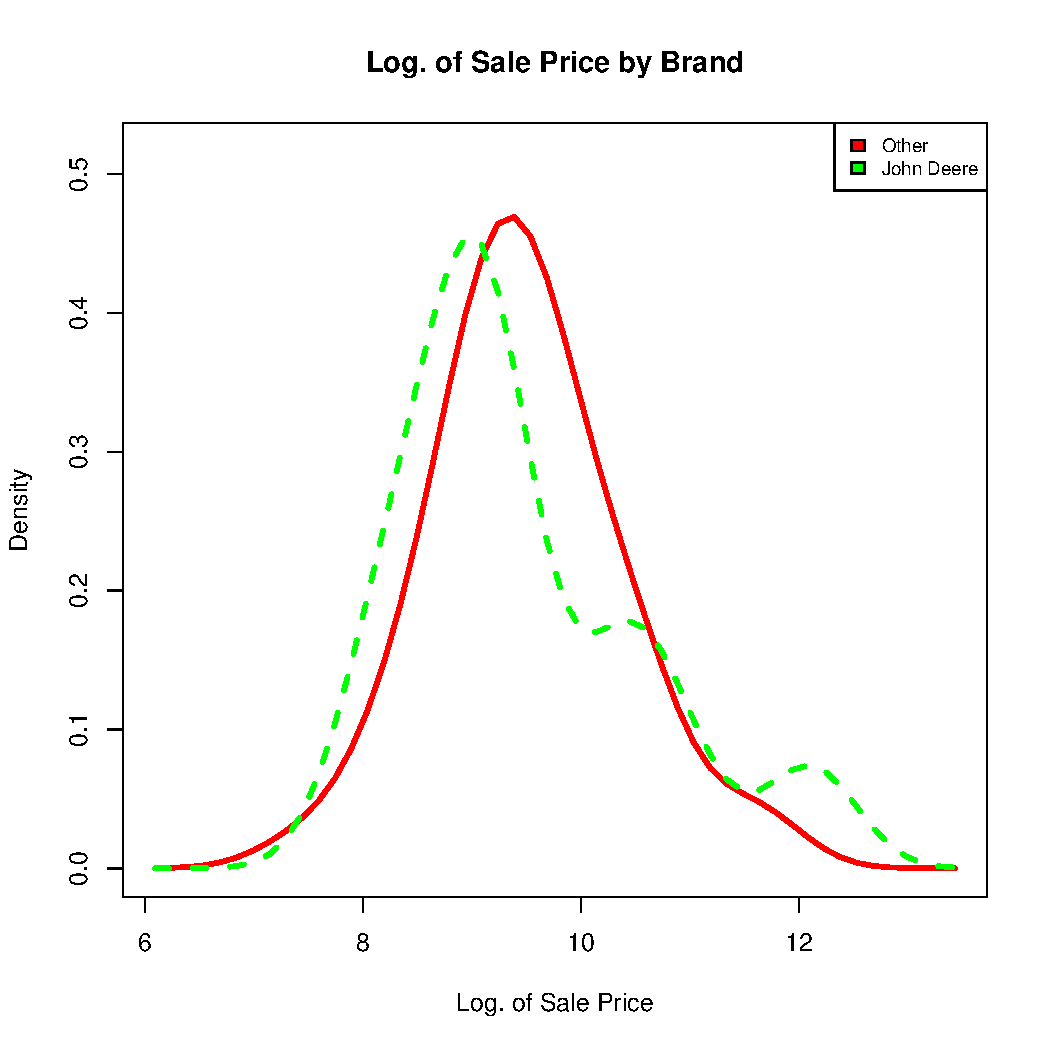
\includegraphics[scale = 0.5, keepaspectratio=true]{../Figures/dens_by_brand}
  \caption{Densities of Log. Tractor Prices by Brand} \label{fig:dens_by_brand}
\end{figure}


\pagebreak
\subsection{Comparison By Season of Sale}

Figure \ref{fig:dens_by_season} shows
the densities of the logarithm of sales price,
separated by the season of the year in which they were sold.
The figure was generated by the following code.
%
\vfill

\begin{lstlisting}[language=R]
plot(density(tractor_sales[tractor_sales[, 'fall'] == 1, 'log_saleprice']),
     col = 'orange',
     lwd = 3,
     xlim = c(min(tractor_sales[, 'log_saleprice']),
              max(tractor_sales[, 'log_saleprice'])),
     main = 'Log. of Sale Price by Season of Sale')
# Plot the rest.
lines(density(tractor_sales[tractor_sales[, 'spring'] == 1, 'log_saleprice']),
     col = 'green',
     lwd = 3)
lines(density(tractor_sales[tractor_sales[, 'summer'] == 1, 'log_saleprice']),
      col = 'yellow',
      lwd = 3)
lines(density(tractor_sales[tractor_sales[, 'winter'] == 1, 'log_saleprice']),
      col = 'blue',
      lwd = 3)
legend('topright',
       c('Spring', 'Summer', 'Fall', 'Winter'),
       fill = c('green', 'yellow', 'orange', 'blue'),
       cex = 0.65)
\end{lstlisting}

\pagebreak
We see that the distribution of sales is similar
during summer and fall (yellow and orange, respectively)
with some bunching in the upper tail.
We also see more variance in the sale price in winter,
shown in blue.
In the spring, shown in green, the mode of the distribution
is higher.

\begin{figure}[h!]
  \centering
  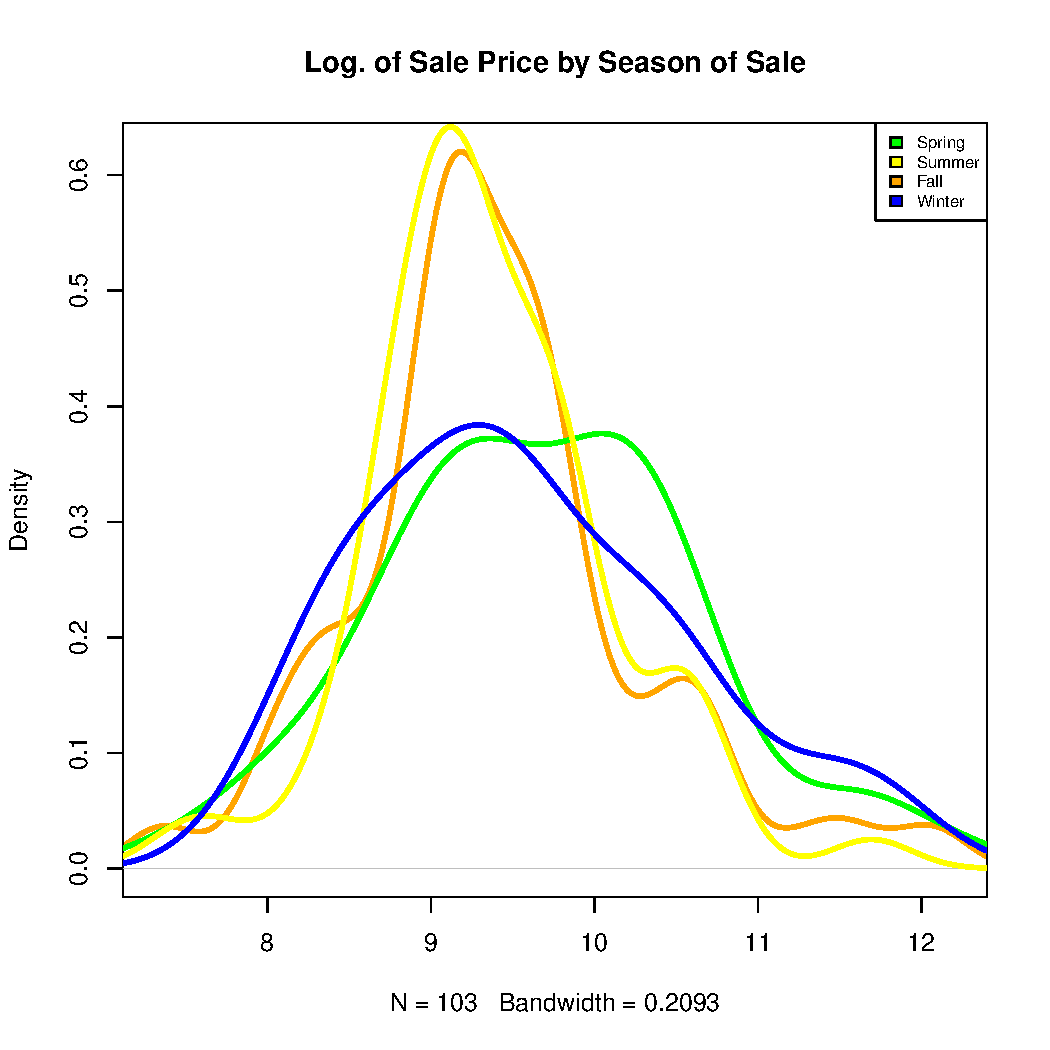
\includegraphics[scale = 0.5, keepaspectratio=true]{../Figures/dens_by_season}
  \caption{Relative Histogram of Tractor Prices} \label{fig:dens_by_season}
\end{figure}


\pagebreak
\section{Sales Volume By Brand and Season of Sale}

Figure \ref{fig:brand_and_season_sales}
shows a spinogram of the number of sales
by brand and the time of year the tractor is sold.
It is generated by the following code.

\begin{lstlisting}[language=R]
# Create a table and plot it in a spinogram.
counts <- table(tractor_sales[, 'season'],
                tractor_sales[, 'JD'])

# Plot the spinogram.
spine(counts,
      main = "Spinogram of Sales by Brand and Season")
\end{lstlisting}

The code block first tabulates the number of sales by
season of sale and whether or not the brand is John Deere.
These counts are shown in Table \ref{tab:brand_and_season_sales}.

       John Deere Other
Fall           14    89
Spring          9    53
Summer          6    58
Winter         10    37


\pagebreak
It appears that sales of John Deere tractors are fairly evenly
distributed throughout the year,
with more sales of John Deere tractors in the winter months
and a fewer sales in the summer.


\begin{figure}[h!]
  \centering
  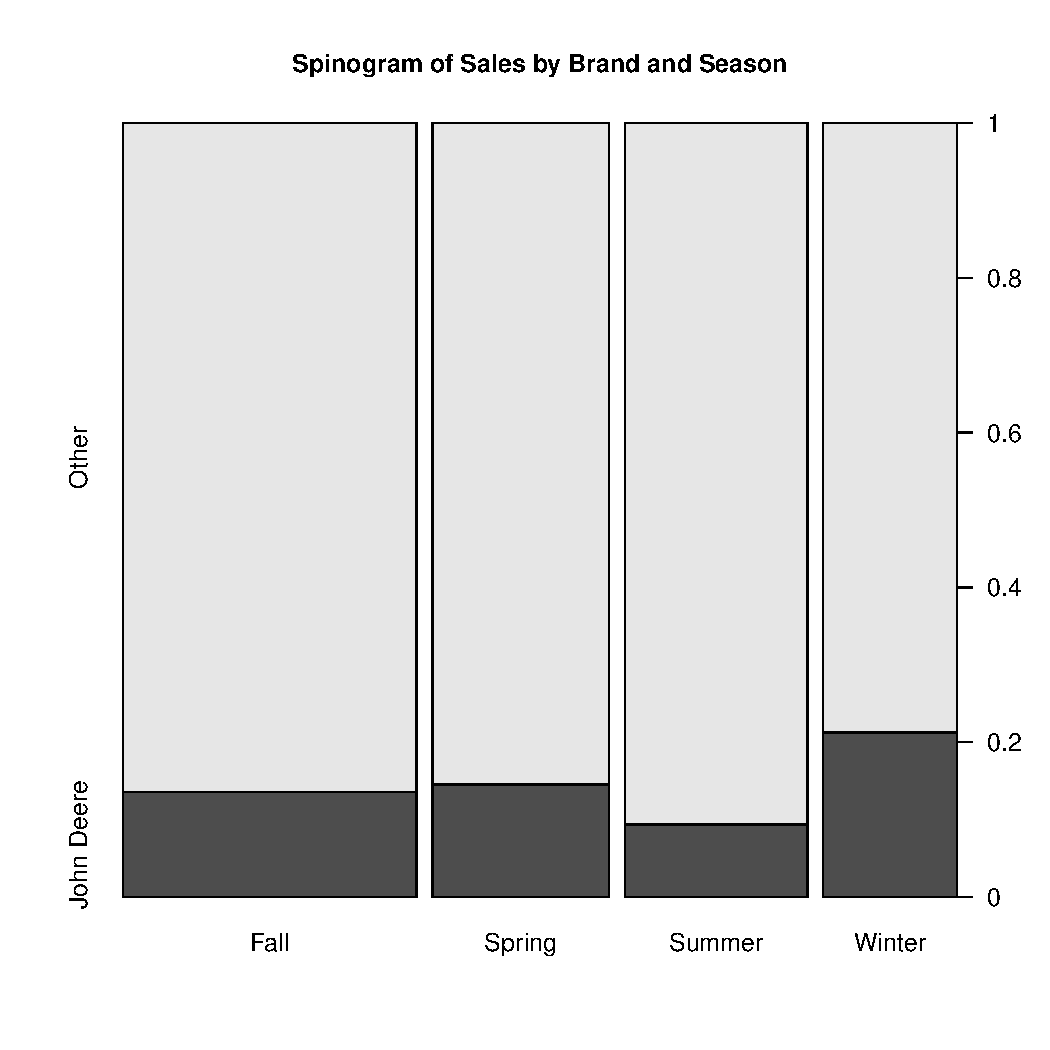
\includegraphics[scale = 0.5, keepaspectratio=true]{../Figures/brand_and_season_sales}
  \caption{Sales Volume of Tractor Prices by Brand and Season of Sale} \label{fig:brand_and_season_sales}
\end{figure}




\pagebreak
\section{Scatterplot Matrix of Numeric Variables}

Figure \ref{fig:scatter_matrix}
shows a scatterplot of the numeric variables in the dataset,
which include
the age in years, the number of engine hours of use,
the number of horsepower produced by the engine,
and the logarithm of the tractor prices.
The \texttt{gclus} package was used to cluster the
correlation matrix to color code by strength of correlation.
The correlation matrix is shown in Table \ref{tab:correlation}.

              Log. of Price Horsepower         Age Engine Hours
Log. of Price    1.00000000 0.64850242 -0.44054234  -0.04583549
Horsepower       0.64850242 1.00000000  0.03884978   0.37778287
Age             -0.44054234 0.03884978  1.00000000   0.55903832
Engine Hours    -0.04583549 0.37778287  0.55903832   1.00000000


The correlation matrix amd the scatterplot matrix
were generated by the following code.

\begin{lstlisting}[language=R]
# Create a covariance matrix and determine
# parameters for scattergraph matrix.
mydata <- tractor_sales[c(13, 2, 3, 4)]
mydata.corr <- abs(cor(mydata))
mycolors <- dmat.color(mydata.corr)
# Order by magnitude of correlation.
myorder <- order.single(mydata.corr)

# Plot the scatterplot matrix.
cpairs(mydata,
       myorder,
       panel.colors = mycolors,
       gap = 0.5,
       main = c('Scatterplot Matrix Colored by Correlation')
)
\end{lstlisting}


\pagebreak
Horsepower and the logarithm of sale price have strong positive correlation, which is shown in red,
suggesting that tractors with more horsepower are more valuable.
Age and engine hours are also highly correlated
as older tractors have likely been used for more hours.
We also see a modest negative correlation between prices and age,
which makes sense since newer tractors may have new features and may be more reliable.
There appears to be little relation between the
age of a tractor and the horsepower produced by the engine.

\begin{figure}[h!]
  \centering
  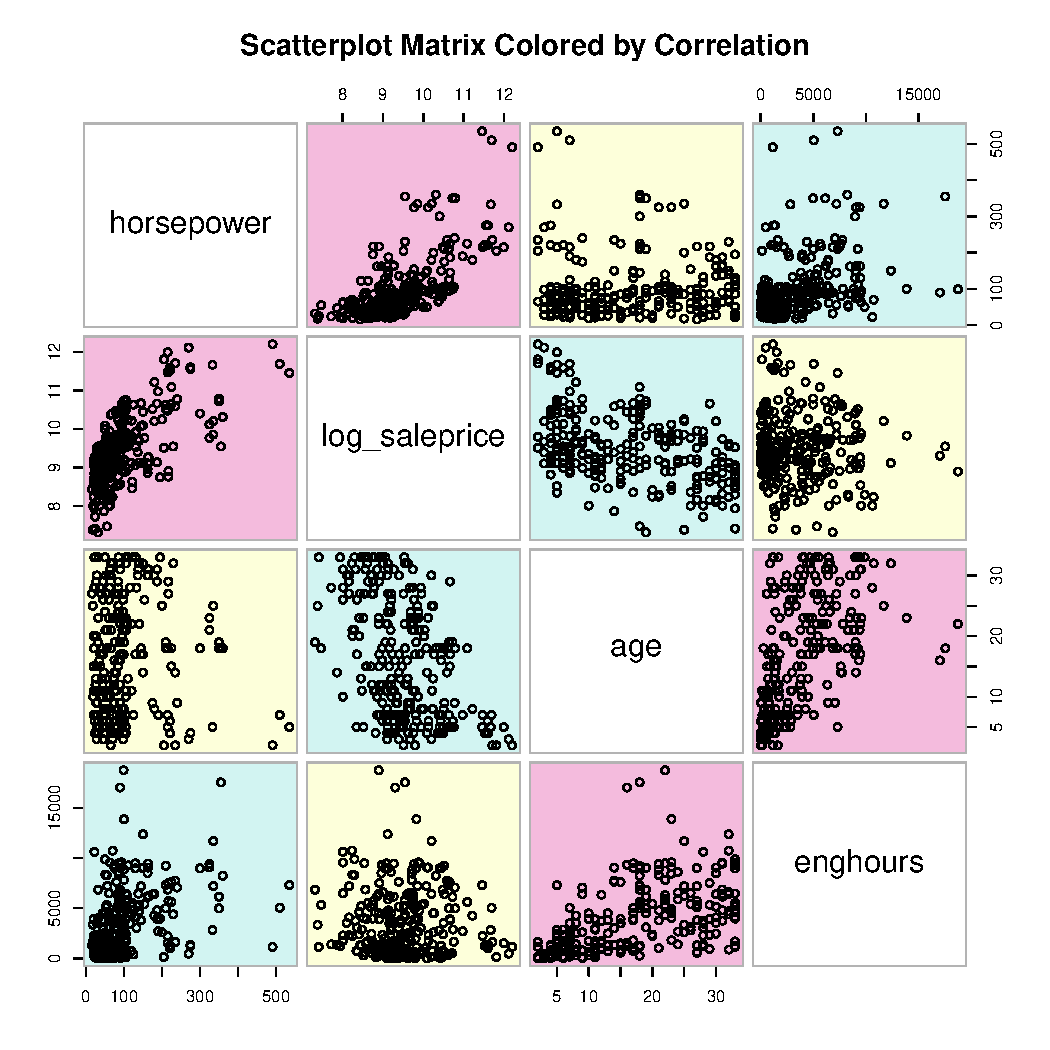
\includegraphics[scale = 0.5, keepaspectratio=true]{../Figures/scatter_matrix}
  \caption{Scatterplot Matrix Colored by Strength of Correlation} \label{fig:scatter_matrix}
\end{figure}



\pagebreak
\section{Relationship between Prices, Horsepower and Age}


Figure \ref{fig:bubble_plot}
shows a bubble plot,
which is a form of scatterplot in which the size of the dots (the ``bubbles'')
represent another variable.
This analysis is based on the above investigation
of the numeric variables in the dataset,
which include
the age in years, the number of engine hours of use,
the number of horsepower produced by the engine,
and the logarithm of the tractor prices.
The logarithm of the tractor prices are shown in the vertical axis,
the age of the tractor is on the horizontal axis,
and the area of each bubble is proportional
to the horsepower of the tractor's engine.
The bubbleplot is
generated by the following code.

\vfill

\begin{lstlisting}[language=R]
# Calculate the radius of the bubbles
# so that the area represents horsepowwer.
r <- sqrt(tractor_sales[, 'horsepower']/pi)

# Plot the bubble plot.
fig_file_name <- 'bubble_plot.pdf'
out_file_name <- sprintf('%s/%s', fig_dir, fig_file_name)
pdf(out_file_name)
symbols(tractor_sales[, 'age'],
        tractor_sales[, 'log_saleprice'],
        r,
        inches=0.30, fg="white", bg="lightblue",
        main = "Bubble Plot with point size proportional to horsepower",
        ylab = "Log. of Sale Price",
        xlab = "Age of Tractor (years)")
\end{lstlisting}


\pagebreak

There appears to be a negative relationship between
the age of a tractor and the sale price.
Also, many of the largest bubbles are concentrated at the higher end of
the price range at each age level.
These findings confirm the results found above in the scatterplots
and covariance matrix.
Together these results indicate that these variables should be included
in some form within a regression model.

\begin{figure}[h!]
  \centering
  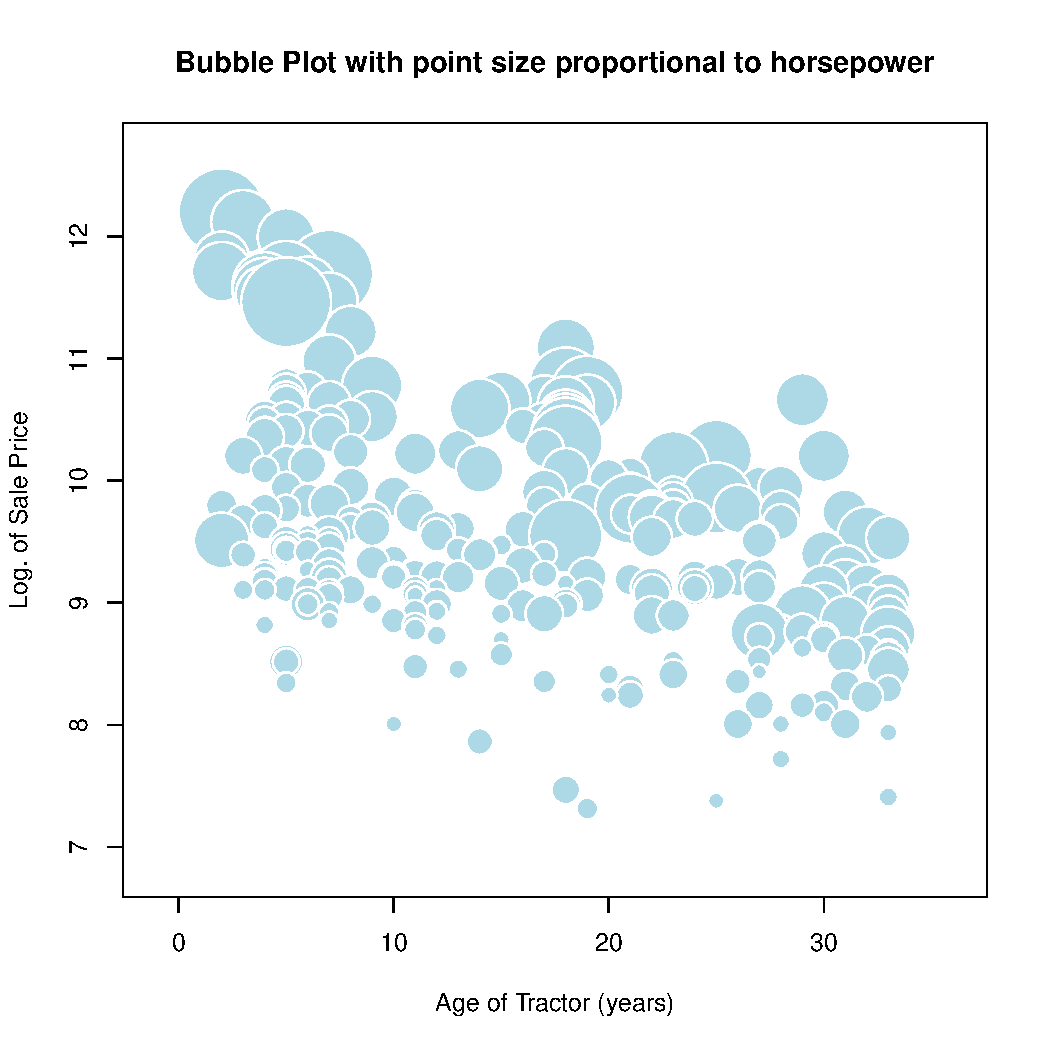
\includegraphics[scale = 0.5, keepaspectratio=true]{../Figures/bubble_plot}
  \caption{Bubble Plot with Point Size Proportional to Horsepower} \label{fig:bubble_plot}
\end{figure}




%%%%%%%%%%%%%%%%%%%%%%%%%%%%%%%%%%%%%%%%
\end{document}
%%%%%%%%%%%%%%%%%%%%%%%%%%%%%%%%%%%%%%%%


\pagebreak
\documentclass[11pt]{paper}
\usepackage{palatino}
\usepackage{amsfonts,amsmath,amssymb}
% \usepackage{graphicx}

\usepackage{listings}
\usepackage{textcomp}
\usepackage{color}

\definecolor{dkgreen}{rgb}{0,0.6,0}
\definecolor{gray}{rgb}{0.5,0.5,0.5}
\definecolor{mauve}{rgb}{0.58,0,0.82}

\lstset{frame=tb,
  language=R,
  aboveskip=3mm,
  belowskip=3mm,
  showstringspaces=false,
  columns=flexible,
  basicstyle={\small\ttfamily},
  numbers=none,
  numberstyle=\tiny\color{gray},
  keywordstyle=\color{blue},
  commentstyle=\color{dkgreen},
  stringstyle=\color{mauve},
  breaklines=true,
  breakatwhitespace=true,
  tabsize=3
}



\ifx\pdftexversion\undefined
    \usepackage[dvips]{graphicx}
\else
    \usepackage[pdftex]{graphicx}
    \usepackage{epstopdf}
    \epstopdfsetup{suffix=}
\fi

\usepackage{subfig}

\begin{document}

%%%%%%%%%%%%%%%%%%%%%%%%%%%%%%%%%%%%%%%%
% Problem Set 6
%%%%%%%%%%%%%%%%%%%%%%%%%%%%%%%%%%%%%%%%

\pagestyle{empty}
{\noindent\bf Spring 2021 \hfill Firstname M.~Lastname}
\vskip 16pt
\centerline{\bf University of Central Florida}
\centerline{\bf College of Business}
\vskip 16pt
\centerline{\bf QMB 6911}
\centerline{\bf Capstone Project in Business Analytics}
\vskip 10pt
\centerline{\bf Solutions:  Problem Set \#7}
\vskip 32pt
\noindent

\section{Data Description}

This analysis follows the script \texttt{Tractor\_Reg\_Model.R} to produce a more accurate model for used tractor prices with the data from \texttt{TRACTOR7.csv} in the \texttt{Data} folder. 
The dataset includes the following variables.
\begin{table}[h!]
\begin{tabular}{l l l}

$saleprice_i$ & = & the price paid for tractor $i$ in dollars \\
% 
$horsepower_i$ & = & the horsepower of tractor $i$ \\
$age_i$ & = & the number of years since tractor $i$ was manufactured  \\
$enghours_i$ & = & the number of hours of use recorded for tractor $i$  \\
$diesel_i$ & = & an indicator of whether tractor $i$ runs on diesel fuel \\ %, $0$ otherwise \\
$fwd_i$ & = & an indicator of whether tractor $i$ has four-wheel drive \\ %, $0$ otherwise \\
$manual_i$ & = & an indicator of whether tractor $i$ has a manual transmission \\ %, $0$ otherwise \\
$johndeere_i$ & = & an indicator of whether tractor $i$ is manufactured by John Deere \\ %, $0$ otherwise \\
$cab_i$ & = & an indicator of whether tractor $i$ has an enclosed cab \\ %, $0$ otherwise \\
% 
$spring_i$ & = & an indicator of whether tractor $i$ was sold in April or May \\ %, $0$ otherwise \\
$summer_i$ & = & an indicator of whether tractor $i$ was sold between June and September \\ %, $0$ otherwise \\
$winter_i$ & = & an indicator of whether tractor $i$ was sold between December and March \\ %, $0$ otherwise \\

\end{tabular}
\end{table}
%

I will first estimate a model with our choices of functional form, and then consider exclusions of insignificant variables from the full model. 
This approach allows for inclusion of possibly irrelevant variables and avoids excluding any relevant variables. 


%%%%%%%%%%%%%%%%%%%%%%%%%%%%%%%%%%%%%%%%
% Choosing the Dependent Variable
%%%%%%%%%%%%%%%%%%%%%%%%%%%%%%%%%%%%%%%%


\pagebreak
\section{Choosing the Dependent Variable}

\subsection{Univariate Analysis}

Figure \ref{fig:hist_price} shows  a histogram of tractor prices.
The distribution is highly skewed to the right, 
with most tractors selling for about \$10,000 or less,
and very few tractors priced above \$50,000.



\begin{figure}[h!]
  \centering
  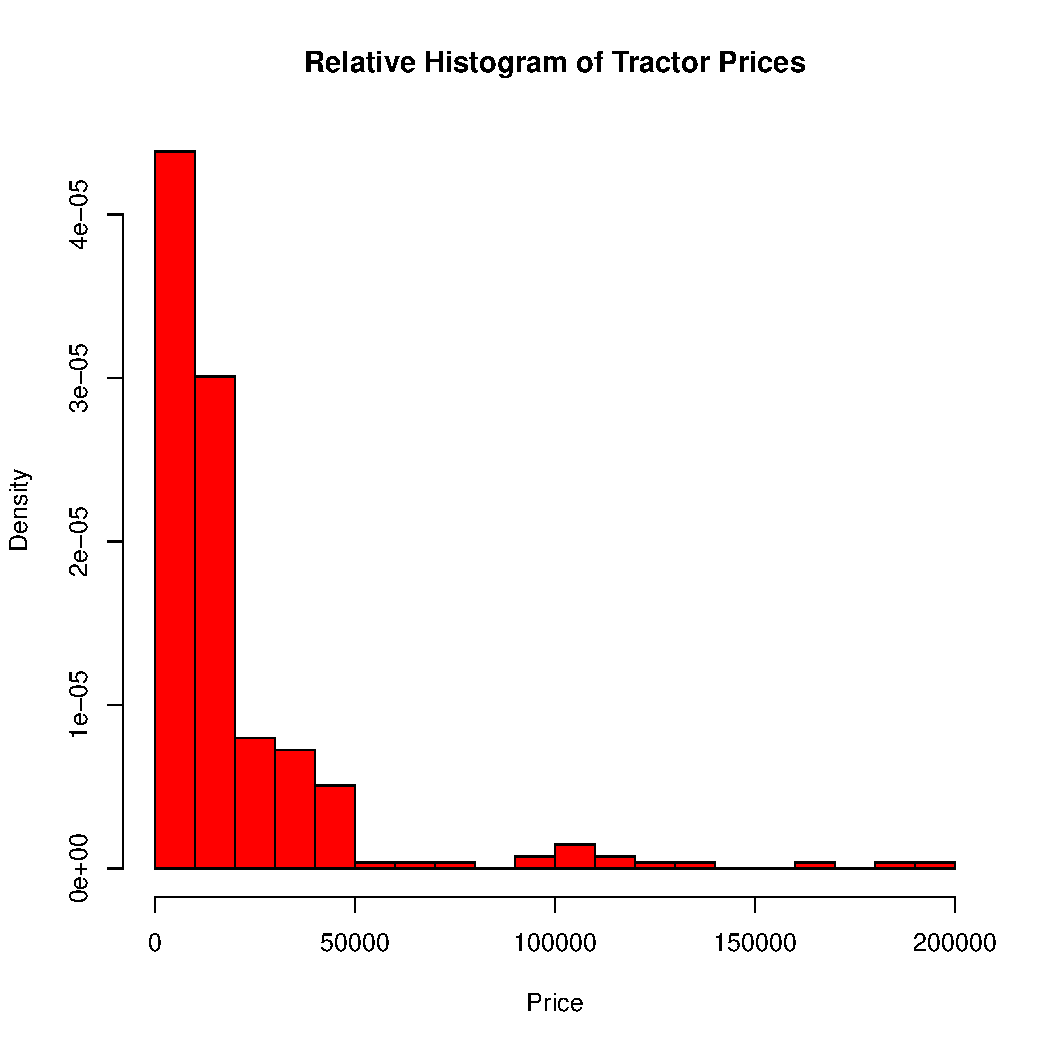
\includegraphics[scale = 0.5, keepaspectratio=true]{../Figures/hist_price}
  \caption{Histogram of Tractor Prices} \label{fig:hist_price}
\end{figure}



\pagebreak
As a comparison, Figure \ref{fig:hist_log_price} shows the histogram of the natural logarithm of
price.

\begin{figure}[h!]
  \centering
  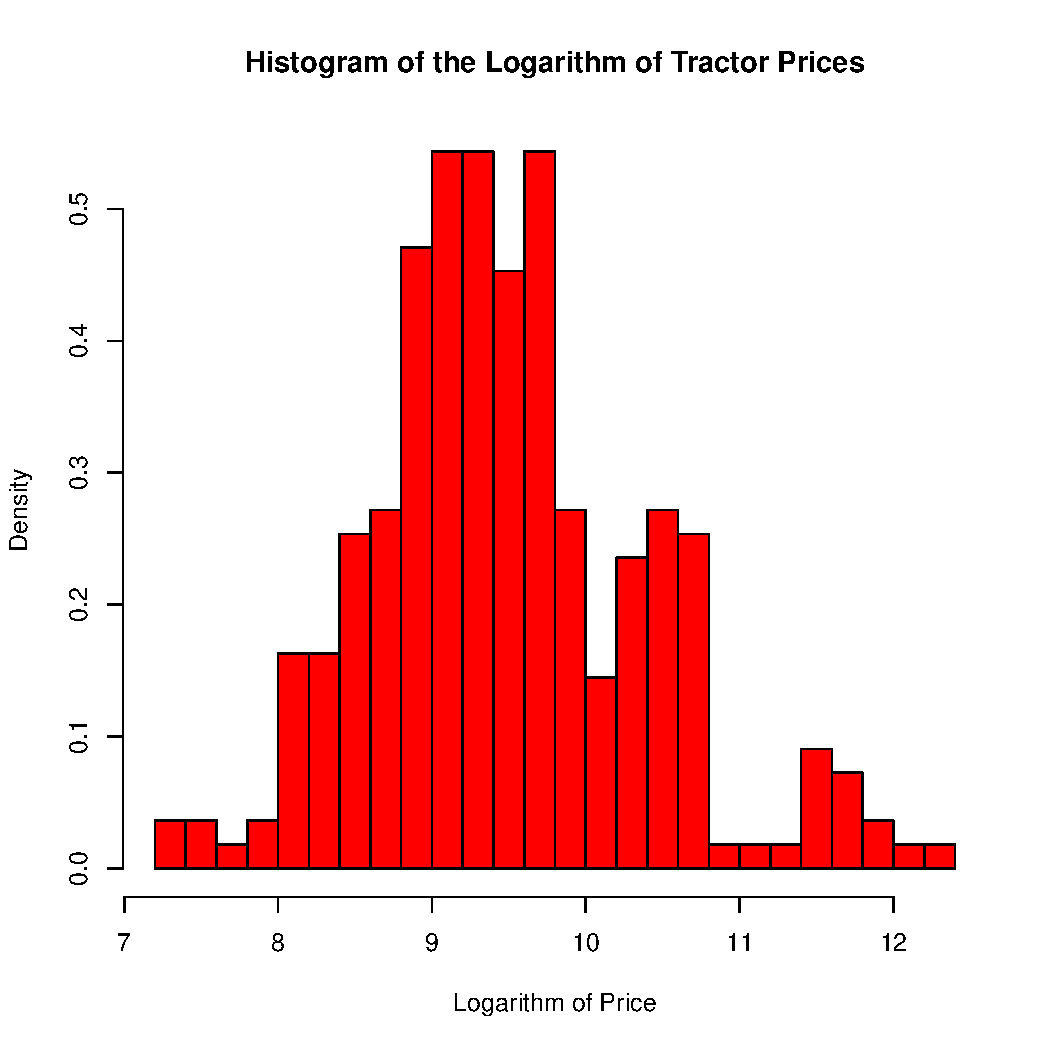
\includegraphics[scale = 0.5, keepaspectratio=true]{../Figures/hist_log_price}
  \caption{Histogram of the Logarithm of Tractor Prices} \label{fig:hist_log_price}
\end{figure}

This is much better behaved. The distribution looks almost normal. 
So far it looks as if the logarithm of the sale price
is the more promising variable.
Another approach to making this decision is
to build the model and judge the validity of the results.



%%%%%%%%%%%%%%%%%%%%%%%%%%%%%%%%%%%%%%%%
% Linear Regression Models
%%%%%%%%%%%%%%%%%%%%%%%%%%%%%%%%%%%%%%%%


\pagebreak
\subsection{Initial Regression Models of Tractor Prices}

\subsubsection{Predicting Price Levels}

First, I will build a model of the price of a used tractor, 
ignoring the above evidence that the distribution is highly skewed. 


\begin{table}
\begin{center}
\begin{tabular}{l c}
\hline
 & Model 1 \\
\hline
(Intercept) & $11670.41^{*}$   \\
            & $(4519.29)$      \\
horsepower  & $246.40^{***}$   \\
            & $(13.98)$        \\
age         & $-674.64^{***}$  \\
            & $(149.00)$       \\
enghours    & $-1.76^{***}$    \\
            & $(0.40)$         \\
diesel      & $2731.97$        \\
            & $(3996.05)$      \\
fwd         & $2570.57$        \\
            & $(2427.51)$      \\
manual      & $-3713.28$       \\
            & $(2586.96)$      \\
johndeere   & $12194.23^{***}$ \\
            & $(2979.91)$      \\
spring      & $-1721.01$       \\
            & $(2716.03)$      \\
summer      & $-5569.46^{*}$   \\
            & $(2654.94)$      \\
winter      & $-1541.99$       \\
            & $(2981.31)$      \\
\hline
R$^2$       & $0.65$           \\
Adj. R$^2$  & $0.63$           \\
Num. obs.   & $276$            \\
\hline
\multicolumn{2}{l}{\scriptsize{$^{***}p<0.001$; $^{**}p<0.01$; $^{*}p<0.05$}}
\end{tabular}
\caption{Dollar Value of Tractor Prices}
\label{tab:price_reg_1}
\end{center}
\end{table}


The results in Table \ref{tab:price_reg_1}
shows the effect of the variables on the dollar price of the
used tractors. 

From the coefficients in the table, 
it appears that a John Deere tractor sells for 
\$12,200 more than an equivalent tractor of another brand. 
This prediction applies equally for tractors all across the spectrum, from the 
To put a finer point on it, 
a 16 horsepower lawn tractor that would otherwise sell for \$2,000 is expected to command \$14,200 if it is a John Deere.
Clearly, this is an unreasonable expectation and
a quick search on your browser will confirm that the John Deere premium is more modest. 


\pagebreak
\subsubsection{Predicting Logarithm of Prices}

Next, I will build a model of the logarithm of the price 
of a used tractor, 
which is consistent with the univariate analysis we conducted earlier. 


\begin{table}
\begin{center}
\begin{tabular}{l c}
\hline
 & Model 1 \\
\hline
(Intercept) & $8.76953^{***}$  \\
            & $(0.13528)$      \\
horsepower  & $0.00654^{***}$  \\
            & $(0.00042)$      \\
age         & $-0.02754^{***}$ \\
            & $(0.00446)$      \\
enghours    & $-0.00002$       \\
            & $(0.00001)$      \\
diesel      & $0.49917^{***}$  \\
            & $(0.11962)$      \\
fwd         & $0.35672^{***}$  \\
            & $(0.07266)$      \\
manual      & $-0.12167$       \\
            & $(0.07744)$      \\
johndeere   & $0.17253$        \\
            & $(0.08920)$      \\
spring      & $-0.03210$       \\
            & $(0.08130)$      \\
summer      & $-0.11876$       \\
            & $(0.07947)$      \\
winter      & $0.04009$        \\
            & $(0.08924)$      \\
\hline
R$^2$       & $0.69709$        \\
Adj. R$^2$  & $0.68566$        \\
Num. obs.   & $276$            \\
\hline
\multicolumn{2}{l}{\scriptsize{$^{***}p<0.001$; $^{**}p<0.01$; $^{*}p<0.05$}}
\end{tabular}
\caption{Logarithm of Tractor Prices}
\label{tab:log_price_reg_2}
\end{center}
\end{table}


The results in Table \ref{tab:log_price_reg_2}
shows the effect of the variables on the logarithm of the dollar price of the used tractors. 
This specification calculates coefficients that 
approximately represent percentage changes in 
tractor prices. 

From the coefficients in the table, 
it appears that a John Deere tractor sells for 
17\% more than an equivalent tractor of another brand. 
That is, a tractor worth \$1,700 would sell
for \$2,000 if it is a John Deere, 
which is clearly more reasonable. 
This more sensible interpretation supports 
the strategy of modeling the 
logarithm of the tractor price. 


%%%%%%%%%%%%%%%%%%%%%%%%%%%%%%%%%%%%%%%%
\clearpage
\section{Model Specification}
%%%%%%%%%%%%%%%%%%%%%%%%%%%%%%%%%%%%%%%%

\subsection{Initial Variable Reduction}

Next, I can refine the model by removing some explanatory variables that do not have string predictive value.
The first candidates are those with coefficients that are not statistically significant. 
The results in Table \ref{tab:reg_reduction}


\begin{table}
\begin{center}
\begin{tabular}{l c c c}
\hline
 & Model 1 & Model 2 & Model 3 \\
\hline
(Intercept) & $8.7695^{***}$  & $8.7559^{***}$  & $8.7787^{***}$  \\
            & $(0.1353)$      & $(0.1284)$      & $(0.1279)$      \\
horsepower  & $0.0065^{***}$  & $0.0066^{***}$  & $0.0065^{***}$  \\
            & $(0.0004)$      & $(0.0004)$      & $(0.0004)$      \\
age         & $-0.0275^{***}$ & $-0.0278^{***}$ & $-0.0297^{***}$ \\
            & $(0.0045)$      & $(0.0044)$      & $(0.0043)$      \\
enghours    & $-0.0000$       & $-0.0000$       & $-0.0000$       \\
            & $(0.0000)$      & $(0.0000)$      & $(0.0000)$      \\
diesel      & $0.4992^{***}$  & $0.4884^{***}$  & $0.4246^{***}$  \\
            & $(0.1196)$      & $(0.1192)$      & $(0.1118)$      \\
fwd         & $0.3567^{***}$  & $0.3492^{***}$  & $0.3416^{***}$  \\
            & $(0.0727)$      & $(0.0721)$      & $(0.0721)$      \\
manual      & $-0.1217$       & $-0.1169$       &                 \\
            & $(0.0774)$      & $(0.0773)$      &                 \\
johndeere   & $0.1725$        & $0.1858^{*}$    & $0.1707$        \\
            & $(0.0892)$      & $(0.0888)$      & $(0.0885)$      \\
spring      & $-0.0321$       &                 &                 \\
            & $(0.0813)$      &                 &                 \\
summer      & $-0.1188$       &                 &                 \\
            & $(0.0795)$      &                 &                 \\
winter      & $0.0401$        &                 &                 \\
            & $(0.0892)$      &                 &                 \\
\hline
R$^2$       & $0.6971$        & $0.6934$        & $0.6907$        \\
Adj. R$^2$  & $0.6857$        & $0.6853$        & $0.6838$        \\
Num. obs.   & $276$           & $276$           & $276$           \\
\hline
\multicolumn{4}{l}{\scriptsize{$^{***}p<0.001$; $^{**}p<0.01$; $^{*}p<0.05$}}
\end{tabular}
\caption{Models for the Log. of Tractor Prices}
\label{tab:reg_reduction}
\end{center}
\end{table}


The first column of Table \ref{tab:reg_reduction}
shows the results from the original model of
the logarithm of tractor prices in Table \ref{tab:log_price_reg_2}. 
The coefficients for seasonal indicators, 
engine hours and manual transmission are not significant.
The John Deere indicator is not significant
but since it is a key empirical question, 
I include it, regardless. 
The second column shows the model without the seasonal indicators. 
We see an improvement in significance of
some variables with minimal loss of predictive ability. 
In the last column, I remove the indicator for manual transmission, with a similar effect on the quality of the model. 
Before making any further changes, 
I will improve the specification of the model
by considering nonlinear specifications. 

\clearpage
\subsection{Quadratic Specification for Horsepower}

Now suppose that 
a used tractor dealer reports that overpowered used tractors are hard to sell, since they consume more fuel. 
This implies that tractor prices often increase with horsepower, up to a point, but beyond that they decrease. 
To incorporate this advice, I created and included a variable for squared horsepower. 

If we expect a decreasing relationship for high values of horsepower, 
this would be characterized by 
a positive coefficient on the horsepower variable and
a negative coefficient on the squared horsepower variable. 

The results of this regression specification are shown in 
Table \ref{tab:reg_sq_horse}. 
% 

\begin{table}
\begin{center}
\begin{tabular}{l c c c}
\hline
 & Model 1 & Model 2 & Model 3 \\
\hline
(Intercept)         & $8.60684^{***}$  & $8.72555^{***}$  & $8.72792^{***}$  \\
                    & $(0.11233)$      & $(0.11156)$      & $(0.10602)$      \\
horsepower          & $0.01504^{***}$  & $0.01115^{***}$  & $0.01112^{***}$  \\
                    & $(0.00097)$      & $(0.00107)$      & $(0.00107)$      \\
squared\_horsepower & $-0.00002^{***}$ & $-0.00001^{***}$ & $-0.00001^{***}$ \\
                    & $(0.00000)$      & $(0.00000)$      & $(0.00000)$      \\
age                 & $-0.03429^{***}$ & $-0.03206^{***}$ & $-0.03233^{***}$ \\
                    & $(0.00374)$      & $(0.00359)$      & $(0.00358)$      \\
enghours            & $-0.00004^{***}$ & $-0.00004^{***}$ & $-0.00004^{***}$ \\
                    & $(0.00001)$      & $(0.00001)$      & $(0.00001)$      \\
diesel              & $0.20070^{*}$    & $0.21453^{*}$    & $0.20350^{*}$    \\
                    & $(0.09975)$      & $(0.09854)$      & $(0.09805)$      \\
fwd                 & $0.31288^{***}$  & $0.27526^{***}$  & $0.26539^{***}$  \\
                    & $(0.06259)$      & $(0.05876)$      & $(0.05820)$      \\
johndeere           & $0.23842^{**}$   & $0.30972^{***}$  & $0.31872^{***}$  \\
                    & $(0.07705)$      & $(0.07236)$      & $(0.07186)$      \\
manual              &                  & $-0.15308^{*}$   & $-0.15015^{*}$   \\
                    &                  & $(0.06209)$      & $(0.06189)$      \\
cab                 &                  & $0.47786^{***}$  & $0.48345^{***}$  \\
                    &                  & $(0.07031)$      & $(0.07003)$      \\
spring              &                  & $-0.04892$       &                  \\
                    &                  & $(0.06506)$      &                  \\
summer              &                  & $-0.05729$       &                  \\
                    &                  & $(0.06379)$      &                  \\
winter              &                  & $0.04596$        &                  \\
                    &                  & $(0.07141)$      &                  \\
\hline
R$^2$               & $0.76838$        & $0.80761$        & $0.80591$        \\
Adj. R$^2$          & $0.76233$        & $0.79884$        & $0.79935$        \\
Num. obs.           & $276$            & $276$            & $276$            \\
\hline
\multicolumn{4}{l}{\scriptsize{$^{***}p<0.001$; $^{**}p<0.01$; $^{*}p<0.05$}}
\end{tabular}
\caption{Quadratic Models for Tractor Prices}
\label{tab:reg_sq_horse}
\end{center}
\end{table}

% 
The squared horsepower variable has a coefficient of $-2.081e-05$, which is nearly ten times as large as the standard error of $2.199e-06$, which is very strong evidence against the null hypothesis of a positive or zero coefficient. 
I conclude that the log of the sale price does decline for large values of horsepower. 


With the squared horsepower variable, the $\bar{R}^2$ has increased substantially to $0.764$, indicating that it is a much stronger model. 
The $F$-statistic is even larger than before, indicating that it is still a better candidate than the simple average log sale price. 
The new squared horsepower variable is statistically significant and the theory behind it is sound, since above a certain point, added horsepower may not improve performance but will cost more to operate. 
This new model is much improved over the previous models with a linear specification for horsepower.

This improved model affords an opportunity
to reconsider other variables in the previous models.
Models 2 and three both include an indicator that the
tractor has an enclosed cab, 
which is also statistically significant. 
The seasonal indicators in Model 2 are not statistically significant under this specification neither. 

\clearpage
\subsection{Quadratic Specification for Horsepower}


The seasonal indicators in Model 2 
of Table \ref{tab:reg_sq_horse}
are not statistically significant individually.
It is possible, however, that jointly, they 
offer an improvement in prediction. 
This can be tested with an $F$-test
to test the joint hypothesis that the time of year has no effect on the sale of tractors. 
%
The null hypothesis is the joint hypothesis that all coefficients on spring, summer and winter are equal to zero. 
The alternative hypothesis is that one of these coefficients is nonzero. 
% 

From the script \texttt{Tractor\_Reg\_Models.R}, the Residual Sum of Squares from the unconstrained model (the model which includes the seasonal indicators) is $41.78944$. 
The constrained model is the one that excludes seasonal indicators and it has a Residual Sum of Squares of $42.15882$.

The $F$-statistic has a value of 

$$ 
\frac{(RSS_M - RSS)/M}{RSS/(N - K - 1)} = \frac{(42.15882 - 41.78944)/3}{RSS/263} = 0.7748937. 
$$

since $N = 276$ observations, $K = 12$ variables and $M = 3$ restrictions, one for each seasonal indicator excluded. 
This is a low value compared to the critical value of $2.60$ for the $F$-statistic with $3$ degrees of freedom in the numerator and $263 (> 120)$ degrees of freedom in the denominator. 
There is no evidence to reject the null that all seasonal indicators have coefficients of zero and conclude that the seasonal indicators should be left out of the model. 
%
The results of the test above indicate that tractor prices do not follow a seasonal pattern


\clearpage
\subsection{Interaction Terms}

\subsubsection{Durability of Engine Types}

Finally, I consider another modification to your model. 
Diesel engines tend to be more durable than gasoline engines. 
This raises the question of whether an additional hour of use affects the value of a diesel tractor differently than for a gasoline tractor. 
This is tested in Model 1 of Table \ref{tab:reg_interactions}. 

	This hypothesis is a test of the \emph{interaction} of the diesel indicator and the slope on engine hours. 
      Given the above result, this test should be conducted with the model that excludes the seasonal indicators. 
The coefficient on \texttt{enghours:diesel} is $4.116e-06$ with a standard error of $2.736e-05$, resulting in a $t$-statistic of $0.150$. 
Since this is a very low value, we cannot reject the null hypothesis that an additional hour of use affects the value of a diesel tractor the same as that for a gasoline tractor. 
Note that this conclusion does not change if you test a one-sided hypothesis.  

Furthermore, the $\bar{R}^2$ statistic decreases with the inclusion of this variable. 
The $F$-statistic is high and statistically significant, indicating that this model is better than the simple average but so is the model without this new variable. 
Finally, the estimates of the other coefficients change very little when this variable is omitted. 
The theory may be sound but there is nothing else to support the inclusion of this new variable. 

% \clearpage
\pagebreak
\subsubsection{Differences in Depreciation by Brand}

The remaining columns of Table \ref{tab:reg_interactions}
show the results of tests for interactions
between the John Deere indicator variable
on the effects of age, engine hours and horsepower. 
There seems to be no evidence for relationships that differ by
brand name. 
In this table, we have investigated several 
individual types of differences by brand. 


\begin{table}
\begin{center}
\begin{tabular}{l c c c c}
\hline
 & Model 1 & Model 2 & Model 3 & Model 4 \\
\hline
(Intercept)          & $8.72858^{***}$  & $8.73093^{***}$  & $8.73093^{***}$  & $8.74493^{***}$  \\
                     & $(0.10630)$      & $(0.10718)$      & $(0.10718)$      & $(0.10691)$      \\
horsepower           & $0.01111^{***}$  & $0.01113^{***}$  & $0.01113^{***}$  & $0.01100^{***}$  \\
                     & $(0.00107)$      & $(0.00107)$      & $(0.00107)$      & $(0.00107)$      \\
squared\_horsepower  & $-0.00001^{***}$ & $-0.00001^{***}$ & $-0.00001^{***}$ & $-0.00001^{***}$ \\
                     & $(0.00000)$      & $(0.00000)$      & $(0.00000)$      & $(0.00000)$      \\
age                  & $-0.03234^{***}$ & $-0.03257^{***}$ & $-0.03257^{***}$ & $-0.03209^{***}$ \\
                     & $(0.00359)$      & $(0.00377)$      & $(0.00377)$      & $(0.00358)$      \\
enghours             & $-0.00004^{***}$ & $-0.00004^{***}$ & $-0.00004^{***}$ & $-0.00004^{***}$ \\
                     & $(0.00001)$      & $(0.00001)$      & $(0.00001)$      & $(0.00001)$      \\
diesel               & $0.20462^{*}$    & $0.20203^{*}$    & $0.20203^{*}$    & $0.19327$        \\
                     & $(0.09849)$      & $(0.09847)$      & $(0.09847)$      & $(0.09835)$      \\
fwd                  & $0.26499^{***}$  & $0.26529^{***}$  & $0.26529^{***}$  & $0.26801^{***}$  \\
                     & $(0.05837)$      & $(0.05831)$      & $(0.05831)$      & $(0.05820)$      \\
manual               & $-0.14954^{*}$   & $-0.14825^{*}$   & $-0.14825^{*}$   & $-0.15257^{*}$   \\
                     & $(0.06213)$      & $(0.06267)$      & $(0.06267)$      & $(0.06188)$      \\
johndeere            & $0.30641^{**}$   & $0.29296^{*}$    & $0.29296^{*}$    & $0.23158^{*}$    \\
                     & $(0.10705)$      & $(0.14255)$      & $(0.14255)$      & $(0.10282)$      \\
cab                  & $0.48420^{***}$  & $0.48386^{***}$  & $0.48386^{***}$  & $0.48270^{***}$  \\
                     & $(0.07033)$      & $(0.07018)$      & $(0.07018)$      & $(0.06998)$      \\
enghours:johndeere   & $0.00000$        &                  &                  &                  \\
                     & $(0.00002)$      &                  &                  &                  \\
age:johndeere        &                  & $0.00146$        & $0.00146$        &                  \\
                     &                  & $(0.00695)$      & $(0.00695)$      &                  \\
horsepower:johndeere &                  &                  &                  & $0.00085$        \\
                     &                  &                  &                  & $(0.00072)$      \\
\hline
R$^2$                & $0.80593$        & $0.80594$        & $0.80594$        & $0.80693$        \\
Adj. R$^2$           & $0.79861$        & $0.79862$        & $0.79862$        & $0.79965$        \\
Num. obs.            & $276$            & $276$            & $276$            & $276$            \\
\hline
\multicolumn{5}{l}{\scriptsize{$^{***}p<0.001$; $^{**}p<0.01$; $^{*}p<0.05$}}
\end{tabular}
\caption{Regression Models for Tractor Prices}
\label{tab:reg_interactions}
\end{center}
\end{table}


To test for many possible differences in 
models by brand of tractor, 
Table \ref{tab:reg_johndeere}
shows the estimates for two separate models
by brand of tractor.
Model 1 shows the estimates for John Deere tractors
and Model 2 represents all other brands. 
The coefficients appear similar across the two subsamples.
Notable differences include the statistical significance for 
the indicators for four-wheel drive, 
manual transmission and an enclosed cab. 
These features seem to change the value of 
other tractors, but perhaps these coefficients are not measured 
accurately for the small sample of 39 
John Deere tractors. 


\begin{table}
\begin{center}
\begin{tabular}{l c c c c c}
\hline
 & Model 1 & Model 2 & Model 3 & Model 4 & Model 5 \\
\hline
(Intercept)         & $8.72792^{***}$  & $8.86706^{***}$  & $9.03796^{***}$  & $8.77320^{***}$  & $8.90792^{***}$  \\
                    & $(0.10602)$      & $(0.22409)$      & $(0.16430)$      & $(0.12450)$      & $(0.08769)$      \\
horsepower          & $0.01112^{***}$  & $0.01502^{***}$  & $0.01580^{***}$  & $0.01032^{***}$  & $0.01057^{***}$  \\
                    & $(0.00107)$      & $(0.00250)$      & $(0.00223)$      & $(0.00119)$      & $(0.00119)$      \\
squared\_horsepower & $-0.00001^{***}$ & $-0.00002^{***}$ & $-0.00002^{***}$ & $-0.00001^{***}$ & $-0.00001^{***}$ \\
                    & $(0.00000)$      & $(0.00000)$      & $(0.00000)$      & $(0.00000)$      & $(0.00000)$      \\
age                 & $-0.03233^{***}$ & $-0.03038^{**}$  & $-0.03295^{***}$ & $-0.03164^{***}$ & $-0.03283^{***}$ \\
                    & $(0.00358)$      & $(0.00914)$      & $(0.00738)$      & $(0.00399)$      & $(0.00392)$      \\
enghours            & $-0.00004^{***}$ & $-0.00006^{*}$   & $-0.00006^{**}$  & $-0.00004^{***}$ & $-0.00004^{***}$ \\
                    & $(0.00001)$      & $(0.00002)$      & $(0.00002)$      & $(0.00001)$      & $(0.00001)$      \\
diesel              & $0.20350^{*}$    & $0.08485$        &                  & $0.18218$        &                  \\
                    & $(0.09805)$      & $(0.18242)$      &                  & $(0.11984)$      &                  \\
fwd                 & $0.26539^{***}$  & $0.12882$        &                  & $0.29072^{***}$  & $0.30003^{***}$  \\
                    & $(0.05820)$      & $(0.15529)$      &                  & $(0.06308)$      & $(0.06296)$      \\
manual              & $-0.15015^{*}$   & $0.06749$        &                  & $-0.17919^{**}$  & $-0.14668^{*}$   \\
                    & $(0.06189)$      & $(0.17288)$      &                  & $(0.06743)$      & $(0.06413)$      \\
johndeere           & $0.31872^{***}$  &                  &                  &                  &                  \\
                    & $(0.07186)$      &                  &                  &                  &                  \\
cab                 & $0.48345^{***}$  & $0.32344$        & $0.38517^{*}$    & $0.51732^{***}$  & $0.52756^{***}$  \\
                    & $(0.07003)$      & $(0.17555)$      & $(0.16365)$      & $(0.07696)$      & $(0.07688)$      \\
\hline
R$^2$               & $0.80591$        & $0.91993$        & $0.91606$        & $0.77992$        & $0.77769$        \\
Adj. R$^2$          & $0.79935$        & $0.89858$        & $0.90334$        & $0.77220$        & $0.77090$        \\
Num. obs.           & $276$            & $39$             & $39$             & $237$            & $237$            \\
\hline
\multicolumn{6}{l}{\scriptsize{$^{***}p<0.001$; $^{**}p<0.01$; $^{*}p<0.05$}}
\end{tabular}
\caption{Separate Models by Brand}
\label{tab:reg_johndeere}
\end{center}
\end{table}


We can also test for all of the differences at the same time
by using an $F$-test. 
In this case, the full, unrestricted model has $K = 2\times9 = 18$ parameters, one for each variable in two models. 
The test that all of the coefficients are the same has $M = 9 - 1 = 8$
restrictions. 
The one restriction fewer accounts for the John Deere indicator
in the full model, 
which allows for two separate intercepts. 
% 
The $F$-statistic has a value of 

$$ 
\frac{(RSS_M - RSS)/M}{RSS/(N - K - 1)} = \frac{(42.15882 - 41.1432)/3}{41.1432/263} = 0.7929991. 
$$

This is also a very low value for the $F$-statistic. 
There is no evidence to reject the null that all 
coefficients are equal across both samples 
and conclude that the John Deere indicator
should be only brand difference left in the model. 

%%%%%%%%%%%%%%%%%%%%%%%%%%%%%%%%%%%%%%%%
\end{document}
%%%%%%%%%%%%%%%%%%%%%%%%%%%%%%%%%%%%%%%%


\pagebreak
\documentclass[11pt]{paper}
\usepackage{palatino}
\usepackage{amsfonts,amsmath,amssymb}
% \usepackage{graphicx}

\usepackage{listings}
\usepackage{textcomp}
\usepackage{color}

\definecolor{dkgreen}{rgb}{0,0.6,0}
\definecolor{gray}{rgb}{0.5,0.5,0.5}
\definecolor{mauve}{rgb}{0.58,0,0.82}

\lstset{frame=tb,
  language=R,
  aboveskip=3mm,
  belowskip=3mm,
  showstringspaces=false,
  columns=flexible,
  basicstyle={\small\ttfamily},
  numbers=none,
  numberstyle=\tiny\color{gray},
  keywordstyle=\color{blue},
  commentstyle=\color{dkgreen},
  stringstyle=\color{mauve},
  breaklines=true,
  breakatwhitespace=true,
  tabsize=3
}



\ifx\pdftexversion\undefined
    \usepackage[dvips]{graphicx}
\else
    \usepackage[pdftex]{graphicx}
    \usepackage{epstopdf}
    \epstopdfsetup{suffix=}
\fi

\usepackage{subfig}


% This allows pdflatex to print the curly quotes in the
% significance codes in the output of the GAM.
\UseRawInputEncoding

\begin{document}

%%%%%%%%%%%%%%%%%%%%%%%%%%%%%%%%%%%%%%%%
% Problem Set 7
%%%%%%%%%%%%%%%%%%%%%%%%%%%%%%%%%%%%%%%%

\pagestyle{empty}
{\noindent\bf Spring 2021 \hfill Firstname M.~Lastname}
\vskip 16pt
\centerline{\bf University of Central Florida}
\centerline{\bf College of Business}
\vskip 16pt
\centerline{\bf QMB 6911}
\centerline{\bf Capstone Project in Business Analytics}
\vskip 10pt
\centerline{\bf Solutions:  Problem Set \#8}
\vskip 32pt
\noindent
% 
\section{Data Description}

This analysis follows the script \texttt{Tractor\_Reg\_Model.R} to produce a more accurate model for used tractor prices with the data from \texttt{TRACTOR7.csv} in the \texttt{Data} folder. 
The dataset includes the following variables.
\begin{table}[h!]
\begin{tabular}{l l l}

$saleprice_i$ & = & the price paid for tractor $i$ in dollars \\
% 
$horsepower_i$ & = & the horsepower of tractor $i$ \\
$age_i$ & = & the number of years since tractor $i$ was manufactured  \\
$enghours_i$ & = & the number of hours of use recorded for tractor $i$  \\
$diesel_i$ & = & an indicator of whether tractor $i$ runs on diesel fuel \\ %, $0$ otherwise \\
$fwd_i$ & = & an indicator of whether tractor $i$ has four-wheel drive \\ %, $0$ otherwise \\
$manual_i$ & = & an indicator of whether tractor $i$ has a manual transmission \\ %, $0$ otherwise \\
$johndeere_i$ & = & an indicator of whether tractor $i$ is manufactured by John Deere \\ %, $0$ otherwise \\
$cab_i$ & = & an indicator of whether tractor $i$ has an enclosed cab \\ %, $0$ otherwise \\
% 
$spring_i$ & = & an indicator of whether tractor $i$ was sold in April or May \\ %, $0$ otherwise \\
$summer_i$ & = & an indicator of whether tractor $i$ was sold between June and September \\ %, $0$ otherwise \\
$winter_i$ & = & an indicator of whether tractor $i$ was sold between December and March \\ %, $0$ otherwise \\

\end{tabular}
\end{table}
%

I will revisit the recommended linear model
from Problem Set \#7, 
which included a quadratic specification for horsepower.
This allowed for an increasing relationship 
between price and horsepower, 
for tractors with low horsepower, 
but a decreasing relationship for the tractors with high horsepower. 
I will investigate this nonlinear relationship
by incorporating a nonparametric specification
for the value of horsepower. 
Similarly, for the other continuous variables engine hours and age, 
to investigate whether these forms of depreciation
are best described with nonlinear forms. 


%%%%%%%%%%%%%%%%%%%%%%%%%%%%%%%%%%%%%%%%
\clearpage
\section{Linear Regression Model}
%%%%%%%%%%%%%%%%%%%%%%%%%%%%%%%%%%%%%%%%

A natural staring point is the recommended linear model
from Problem Set \#7. 

\subsection{Quadratic Specification for Horsepower}

Last week we considered the advice of
a used tractor dealer who reported that overpowered used tractors are hard to sell, since they consume more fuel. 
This implies that tractor prices often increase with horsepower, up to a point, but beyond that they decrease. 
To incorporate this advice, I created and included a variable for squared horsepower. 
A decreasing relationship for high values of horsepower
is characterized by 
a positive coefficient on the horsepower variable and
a negative coefficient on the squared horsepower variable. 

The results of this regression specification are shown in 
Table \ref{tab:reg_sq_horse}. 
% 

\begin{table}
\begin{center}
\begin{tabular}{l c c c}
\hline
 & Model 1 & Model 2 & Model 3 \\
\hline
(Intercept)         & $8.60684^{***}$  & $8.72555^{***}$  & $8.72792^{***}$  \\
                    & $(0.11233)$      & $(0.11156)$      & $(0.10602)$      \\
horsepower          & $0.01504^{***}$  & $0.01115^{***}$  & $0.01112^{***}$  \\
                    & $(0.00097)$      & $(0.00107)$      & $(0.00107)$      \\
squared\_horsepower & $-0.00002^{***}$ & $-0.00001^{***}$ & $-0.00001^{***}$ \\
                    & $(0.00000)$      & $(0.00000)$      & $(0.00000)$      \\
age                 & $-0.03429^{***}$ & $-0.03206^{***}$ & $-0.03233^{***}$ \\
                    & $(0.00374)$      & $(0.00359)$      & $(0.00358)$      \\
enghours            & $-0.00004^{***}$ & $-0.00004^{***}$ & $-0.00004^{***}$ \\
                    & $(0.00001)$      & $(0.00001)$      & $(0.00001)$      \\
diesel              & $0.20070^{*}$    & $0.21453^{*}$    & $0.20350^{*}$    \\
                    & $(0.09975)$      & $(0.09854)$      & $(0.09805)$      \\
fwd                 & $0.31288^{***}$  & $0.27526^{***}$  & $0.26539^{***}$  \\
                    & $(0.06259)$      & $(0.05876)$      & $(0.05820)$      \\
johndeere           & $0.23842^{**}$   & $0.30972^{***}$  & $0.31872^{***}$  \\
                    & $(0.07705)$      & $(0.07236)$      & $(0.07186)$      \\
manual              &                  & $-0.15308^{*}$   & $-0.15015^{*}$   \\
                    &                  & $(0.06209)$      & $(0.06189)$      \\
cab                 &                  & $0.47786^{***}$  & $0.48345^{***}$  \\
                    &                  & $(0.07031)$      & $(0.07003)$      \\
spring              &                  & $-0.04892$       &                  \\
                    &                  & $(0.06506)$      &                  \\
summer              &                  & $-0.05729$       &                  \\
                    &                  & $(0.06379)$      &                  \\
winter              &                  & $0.04596$        &                  \\
                    &                  & $(0.07141)$      &                  \\
\hline
R$^2$               & $0.76838$        & $0.80761$        & $0.80591$        \\
Adj. R$^2$          & $0.76233$        & $0.79884$        & $0.79935$        \\
Num. obs.           & $276$            & $276$            & $276$            \\
\hline
\multicolumn{4}{l}{\scriptsize{$^{***}p<0.001$; $^{**}p<0.01$; $^{*}p<0.05$}}
\end{tabular}
\caption{Quadratic Models for Tractor Prices}
\label{tab:reg_sq_horse}
\end{center}
\end{table}

% 
The squared horsepower variable has a coefficient of $-2.081e-05$, which is nearly ten times as large as the standard error of $2.199e-06$, which is very strong evidence against the null hypothesis of a positive or zero coefficient. 
I conclude that the log of the sale price does decline for large values of horsepower. 


With the squared horsepower variable, the $\bar{R}^2$ is $0.764$, indicating that it is a much stronger model than the others we considered. 
The $F$-statistic is large, indicating that it is a better candidate than the simple average log sale price. 
The new squared horsepower variable is statistically significant and the theory behind it is sound, since above a certain point, added horsepower may not improve performance but will cost more to operate. 
This new model is much improved over the previous models with a linear specification for horsepower.
Next, I will attempt to improve on this specification. 





%%%%%%%%%%%%%%%%%%%%%%%%%%%%%%%%%%%%%%%%
\clearpage
\section{Nonlinear Specifications}
%%%%%%%%%%%%%%%%%%%%%%%%%%%%%%%%%%%%%%%%


% \clearpage
\subsection{Nonparametric Specification for Horsepower}


The specification in 
Table \ref{tab:reg_sq_horse}
assumes a quadratic functional form for
the relationship between price and horsepower. 
To consider the horsepower variable alone, 
while accounting for the effects of other variables, 
one can fit a nonparametric model to the residuals 
from a model of tractor prices, 
after regressing tractor prices on the other variables. 
This leaves only the variation in tractor prices that is not explained by the other variables. 
Going one step further, perform the same transformation to the horsepower variable:
take the residuals from a model of horsepower, 
after regressing horsepower on the other variables. 
This allows a model that would fit exactly the same as if it were estimated within a full model with all variables included. 

The models shown in
Table \ref{tab:reg_sq_horse_fwl}
illustrate this possibility. 
Model 1 is the original model in 
Table \ref{tab:reg_sq_horse}. 
Model 2 is a regression omitting the horsepower variables. 
Model 3 is a regression to predict horsepower with the other explanatory variables in Model 2.
Finally, Model 4 shows the coefficients for horsepower
from a regression of the residuals of Model 2
on the residuals from Model 3. 
Notice that these coefficients match those in Model 1. 
You might notice a slight difference in the standard errors, however, 
because these are calculated assuming coefficients 
for two variables, horsepower and squared horsepower,
rather than the full suite of ten parameters.
This equivalence of the coefficients can be used to fit
nonlinear models between a pair of variables by 
partialing out the effect of the other variables, 
using a mathematical result called the Frisch-Waugh-Lovell (FWL) theorem, 
maned after early statisticians and econometricians who used these methods. 


\begin{table}
\begin{center}
\begin{tabular}{l c c c c c}
\hline
 & Model 1 & Model 2 & Model 3 & Model 4 & Model 5 \\
\hline
(Intercept)          & $8.72792^{***}$  & $9.01091^{***}$  & $27.05189$       & $1269.75517$        &                  \\
                     & $(0.10602)$      & $(0.13785)$      & $(17.13098)$     & $(8102.93510)$      &                  \\
horsepower           & $0.01112^{***}$  &                  &                  &                     &                  \\
                     & $(0.00107)$      &                  &                  &                     &                  \\
squared\_horsepower  & $-0.00001^{***}$ &                  &                  &                     &                  \\
                     & $(0.00000)$      &                  &                  &                     &                  \\
age                  & $-0.03233^{***}$ & $-0.03609^{***}$ & $-1.27409^{*}$   & $-741.49174^{**}$   &                  \\
                     & $(0.00358)$      & $(0.00473)$      & $(0.58819)$      & $(278.21478)$       &                  \\
enghours             & $-0.00004^{***}$ & $-0.00000$       & $0.00735^{***}$  & $2.90344^{***}$     &                  \\
                     & $(0.00001)$      & $(0.00001)$      & $(0.00153)$      & $(0.72137)$         &                  \\
diesel               & $0.20350^{*}$    & $0.32931^{*}$    & $6.21382$        & $-4041.08422$       &                  \\
                     & $(0.09805)$      & $(0.12991)$      & $(16.14428)$     & $(7636.22715)$      &                  \\
fwd                  & $0.26539^{***}$  & $0.34908^{***}$  & $18.48035$       & $8678.65733$        &                  \\
                     & $(0.05820)$      & $(0.07756)$      & $(9.63839)$      & $(4558.94619)$      &                  \\
manual               & $-0.15015^{*}$   & $-0.08564$       & $15.32259$       & $7543.06505$        &                  \\
                     & $(0.06189)$      & $(0.08268)$      & $(10.27470)$     & $(4859.92047)$      &                  \\
johndeere            & $0.31872^{***}$  & $0.37245^{***}$  & $13.28577$       & $6697.80712$        &                  \\
                     & $(0.07186)$      & $(0.09618)$      & $(11.95221)$     & $(5653.38319)$      &                  \\
cab                  & $0.48345^{***}$  & $1.03138^{***}$  & $72.82965^{***}$ & $18662.03208^{***}$ &                  \\
                     & $(0.07003)$      & $(0.07637)$      & $(9.49032)$      & $(4488.91194)$      &                  \\
horsepower\_resid    &                  &                  &                  &                     & $0.01112^{***}$  \\
                     &                  &                  &                  &                     & $(0.00105)$      \\
horsepower\_2\_resid &                  &                  &                  &                     & $-0.00001^{***}$ \\
                     &                  &                  &                  &                     & $(0.00000)$      \\
\hline
R$^2$                & $0.80591$        & $0.64790$        & $0.40004$        & $0.22696$           & $0.44877$        \\
Adj. R$^2$           & $0.79935$        & $0.63871$        & $0.38437$        & $0.20677$           & $0.44474$        \\
Num. obs.            & $276$            & $276$            & $276$            & $276$               & $276$            \\
\hline
\multicolumn{6}{l}{\scriptsize{$^{***}p<0.001$; $^{**}p<0.01$; $^{*}p<0.05$}}
\end{tabular}
\caption{Quadratic Model for Tractor Prices: FWL Regressions}
\label{tab:reg_sq_horse_fwl}
\end{center}
\end{table}


\pagebreak 
To illustrate the fit of the model, 
Figure \ref{fig:dev_vs_horse} shows a scatter plot 
of the residual log prices on horsepower. 
The observations are shown in blue
and the fitted values are shown in red.
The variation in the fitted values results from the 
fact that it is not plotted against the transformed excess horsepower variable used in the regressions.
Still, the quadratic pattern is apparent
and appears to match the data. 

\begin{figure}[h!]
  \centering
  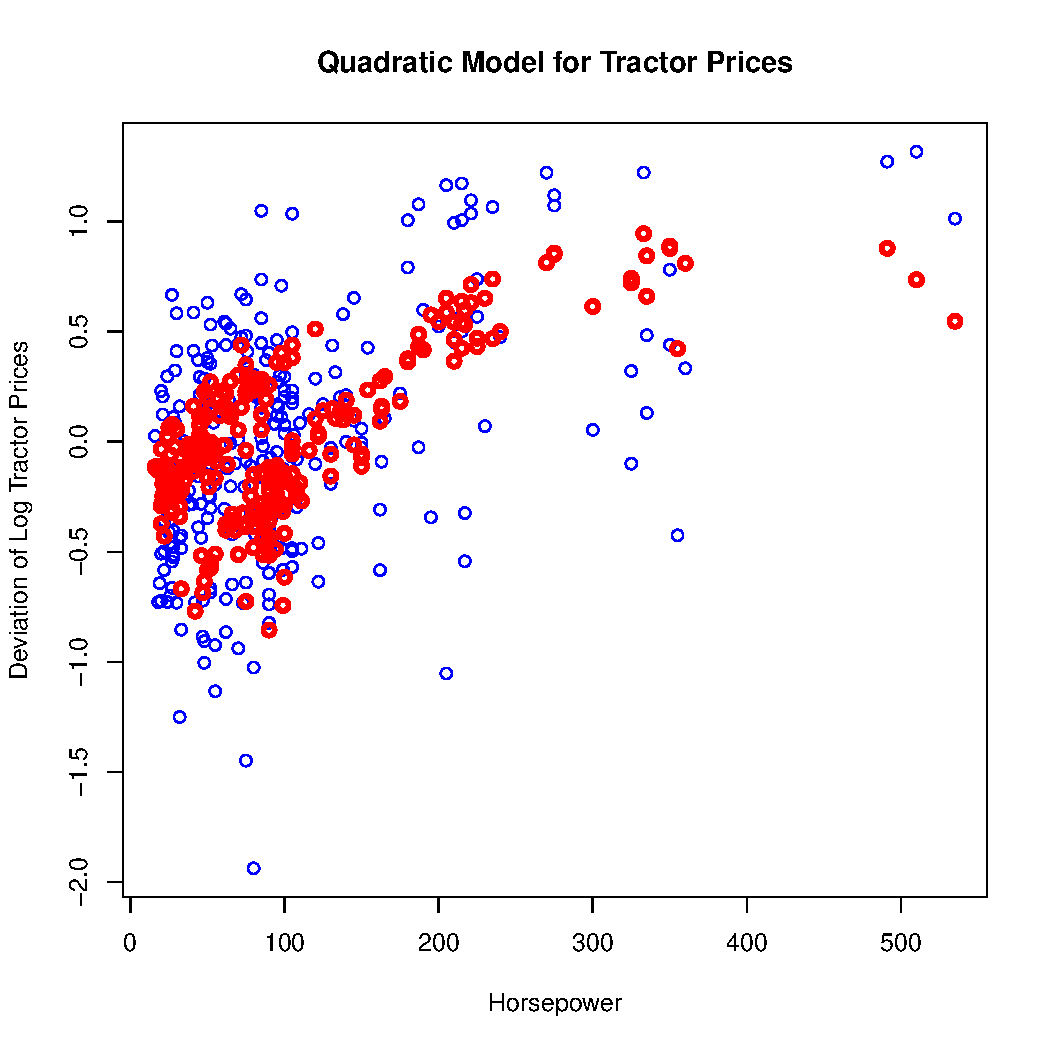
\includegraphics[scale = 0.5, keepaspectratio=true]{../Figures/dev_vs_horse}
  \caption{Linear-Quadratic Model for Tractor Prices} \label{fig:dev_vs_horse}
\end{figure}



\pagebreak
As a comparison, Figure \ref{fig:dev_vs_horse_dev} 
augments the above by showing the plot against the 
residuals from the regression for horsepower:
the ``excess horsepower'' compared to what would be 
expected given the other characteristics of a tractor. 
The quadratic function is more clear from this perspective. 
This time, the variation in the fitted values results from the 
two-dimensional nature of the horsepower variable
when we consider the quadratic form.


\begin{figure}[h!]
  \centering
  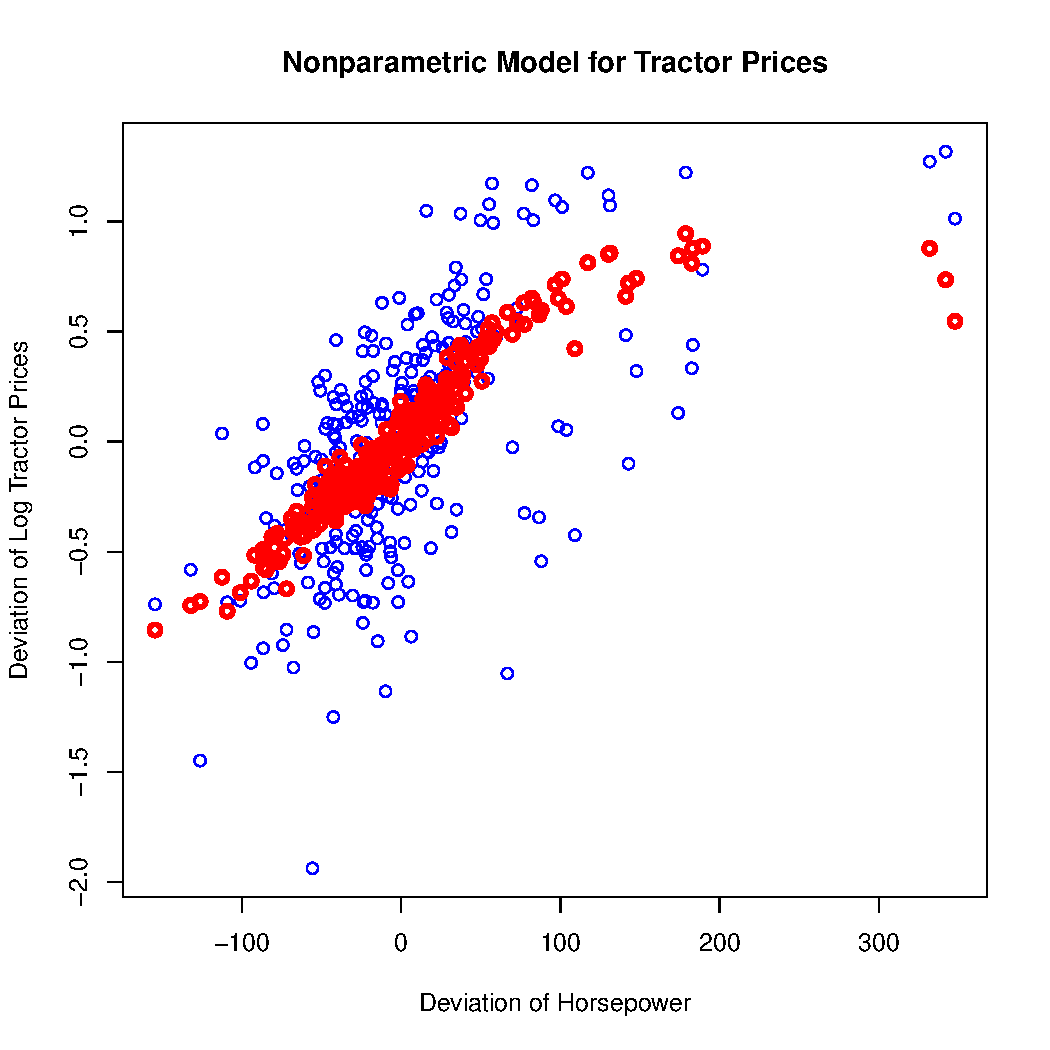
\includegraphics[scale = 0.5, keepaspectratio=true]{../Figures/dev_vs_horse_dev}
  \caption{Linear-Quadratic Model for Tractor Prices: Excess Horsepower} \label{fig:dev_vs_horse_dev}
\end{figure}

\clearpage
Now consider a nonparametric specification for 
the relationship between prices and horsepower.
Figure \ref{fig:dev_np_vs_horse_dev} 
overlays the nonparametric estimate (shown in green) with the above in 
Figure \ref{fig:dev_vs_horse_dev}.
The pattern has more variation in slope but 
closely follows the prediction from the quadratic model. 
So far, it appears that the quadratic form
is close enough.

\begin{figure}[h!]
  \centering
  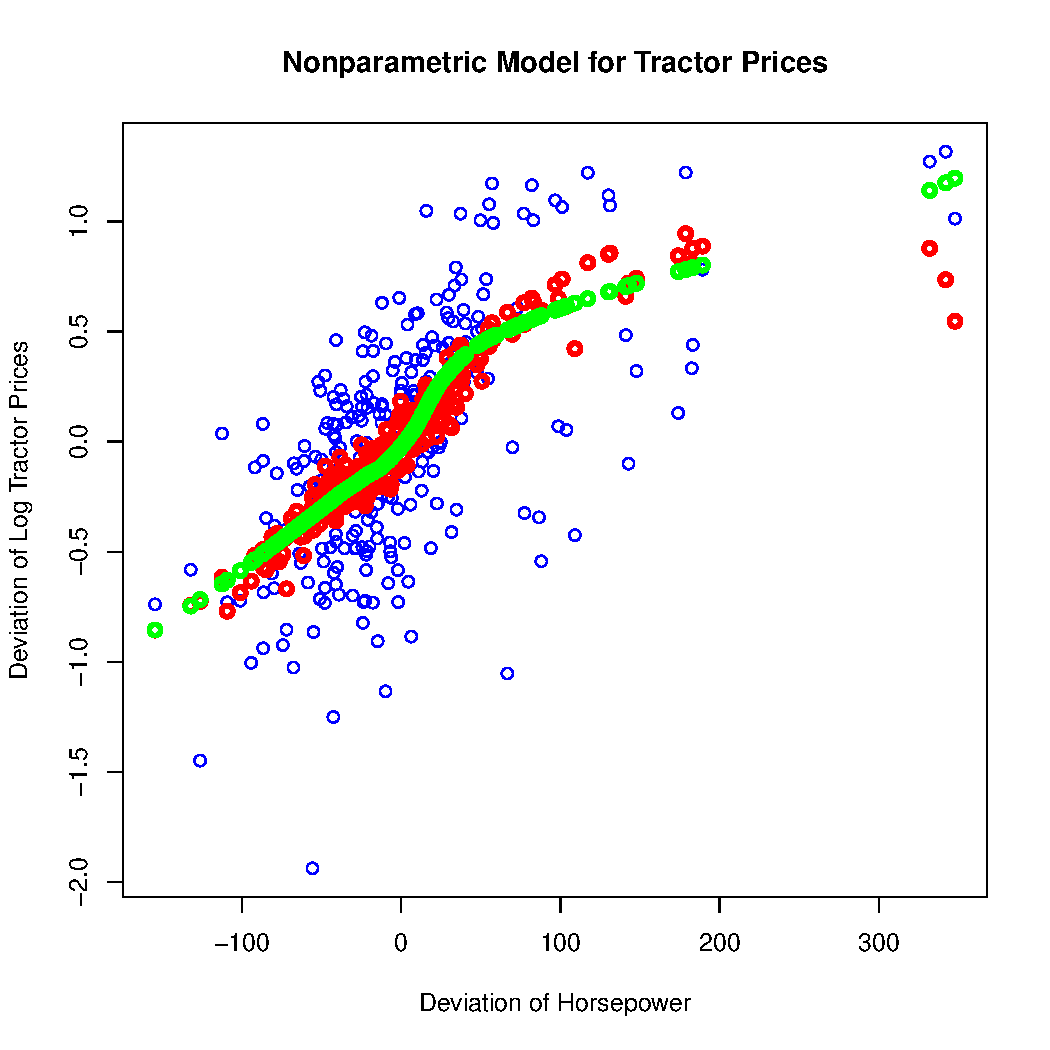
\includegraphics[scale = 0.5, keepaspectratio=true]{../Figures/dev_np_vs_horse_dev}
  \caption{Nonparametric Model for Tractor Prices: Excess Horsepower} \label{fig:dev_np_vs_horse_dev}
\end{figure}

 

\clearpage
Finally, consider a set of nonparametric specifications for 
the relationship between prices and horsepower.
Figure \ref{fig:dev_np_vs_horse_dev_bw} 
overlays other nonparametric estimates with the above in 
Figure \ref{fig:dev_np_vs_horse_dev}.
The points in orange and in magenta represent
alternate models with different degrees of smoothing. 
%
When we estimated probability densities,
we adjusted the bandwidth parameter to fit
with different degrees of smoothness.
The \texttt{loess} method used for the nonparametric method has a span parameter for this function.
The default smoother \texttt{span} (bandwidth parameter) is 0.75.

In the magenta points, with \texttt{span} parameter 0.1, the pattern has more variation in slope but 
closely follows the prediction from the quadratic model. 
The smoother curve in orange 
even more closely represents a quadratic line. 
Again, it appears that the quadratic form
is close enough.
Perhaps the result will be different for other continuous variables in the model.

\begin{figure}[h!]
  \centering
  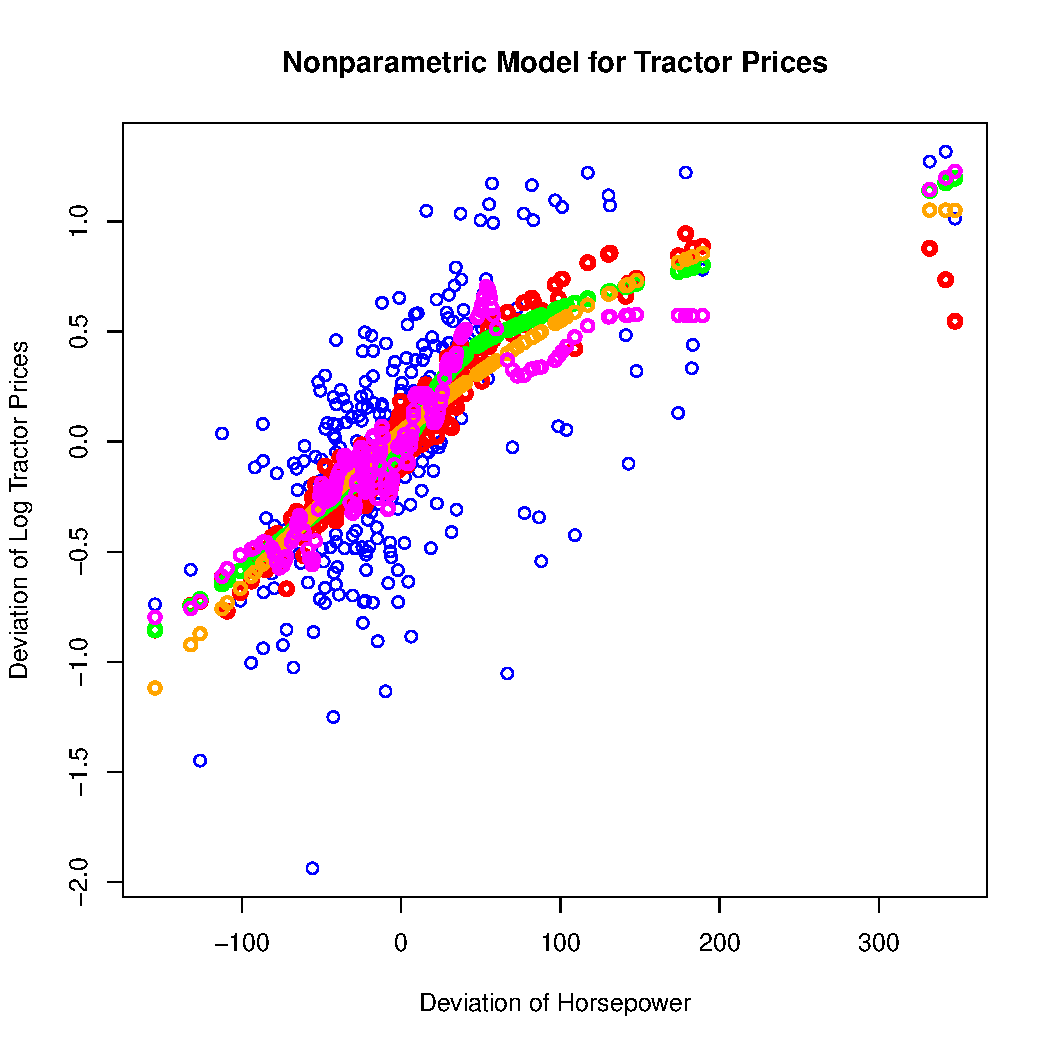
\includegraphics[scale = 0.5, keepaspectratio=true]{../Figures/dev_np_vs_horse_dev_bw}
  \caption{Nonparametric Model for Tractor Prices: Excess Horsepower} \label{fig:dev_np_vs_horse_dev_bw}
\end{figure}





\clearpage
\subsection{Nonparametric Specification for Age}

As above, first conduct FWL regressions 
to reduce the problem to two dimensions. 
The models shown in
Table \ref{tab:reg_age_fwl}
illustrate this possibility. 
Model 1 is the same original model in 
Table \ref{tab:reg_sq_horse}. 
Model 2 is a regression omitting the age variable. 
Model 3 is a regression to predict age with the other explanatory variables in Model 2.
Finally, Model 4 shows the coefficient for age
from a regression of the residuals of Model 2
on the residuals from Model 3. 
Notice that these coefficients match those in Model 1. 


\begin{table}
\begin{center}
\begin{tabular}{l c c c c}
\hline
 & Model 1 & Model 2 & Model 3 & Model 4 \\
\hline
(Intercept)         & $8.72792^{***}$  & $8.25387^{***}$  & $14.66329^{***}$ &                  \\
                    & $(0.10602)$      & $(0.10509)$      & $(1.57457)$      &                  \\
horsepower          & $0.01112^{***}$  & $0.01055^{***}$  & $0.01761$        &                  \\
                    & $(0.00107)$      & $(0.00122)$      & $(0.01821)$      &                  \\
squared\_horsepower & $-0.00001^{***}$ & $-0.00001^{***}$ & $-0.00007$       &                  \\
                    & $(0.00000)$      & $(0.00000)$      & $(0.00004)$      &                  \\
age                 & $-0.03233^{***}$ &                  &                  &                  \\
                    & $(0.00358)$      &                  &                  &                  \\
enghours            & $-0.00004^{***}$ & $-0.00008^{***}$ & $0.00131^{***}$  &                  \\
                    & $(0.00001)$      & $(0.00001)$      & $(0.00014)$      &                  \\
diesel              & $0.20350^{*}$    & $0.32816^{**}$   & $-3.85602^{*}$   &                  \\
                    & $(0.09805)$      & $(0.11075)$      & $(1.65943)$      &                  \\
fwd                 & $0.26539^{***}$  & $0.48826^{***}$  & $-6.89389^{***}$ &                  \\
                    & $(0.05820)$      & $(0.06014)$      & $(0.90112)$      &                  \\
manual              & $-0.15015^{*}$   & $-0.30537^{***}$ & $4.80111^{***}$  &                  \\
                    & $(0.06189)$      & $(0.06784)$      & $(1.01643)$      &                  \\
johndeere           & $0.31872^{***}$  & $0.30073^{***}$  & $0.55646$        &                  \\
                    & $(0.07186)$      & $(0.08196)$      & $(1.22801)$      &                  \\
cab                 & $0.48345^{***}$  & $0.48403^{***}$  & $-0.01803$       &                  \\
                    & $(0.07003)$      & $(0.07990)$      & $(1.19717)$      &                  \\
age\_resid          &                  &                  &                  & $-0.03233^{***}$ \\
                    &                  &                  &                  & $(0.00352)$      \\
\hline
R$^2$               & $0.80591$        & $0.74641$        & $0.51998$        & $0.23464$        \\
Adj. R$^2$          & $0.79935$        & $0.73881$        & $0.50560$        & $0.23186$        \\
Num. obs.           & $276$            & $276$            & $276$            & $276$            \\
\hline
\multicolumn{5}{l}{\scriptsize{$^{***}p<0.001$; $^{**}p<0.01$; $^{*}p<0.05$}}
\end{tabular}
\caption{Linear Model for Age: FWL Regressions}
\label{tab:reg_age_fwl}
\end{center}
\end{table}


\pagebreak 
To illustrate the fit of the model, 
Figure \ref{fig:dev_vs_age} shows a scatter plot 
of the residual log prices on age. 
The observations are shown in blue
and the fitted values are shown in red.
The variation in the fitted values results from the 
fact that it is not plotted against the transformed excess age variable used in the regressions.
Still, the linear pattern is apparent
and appears to match the data. 

\begin{figure}[h!]
  \centering
  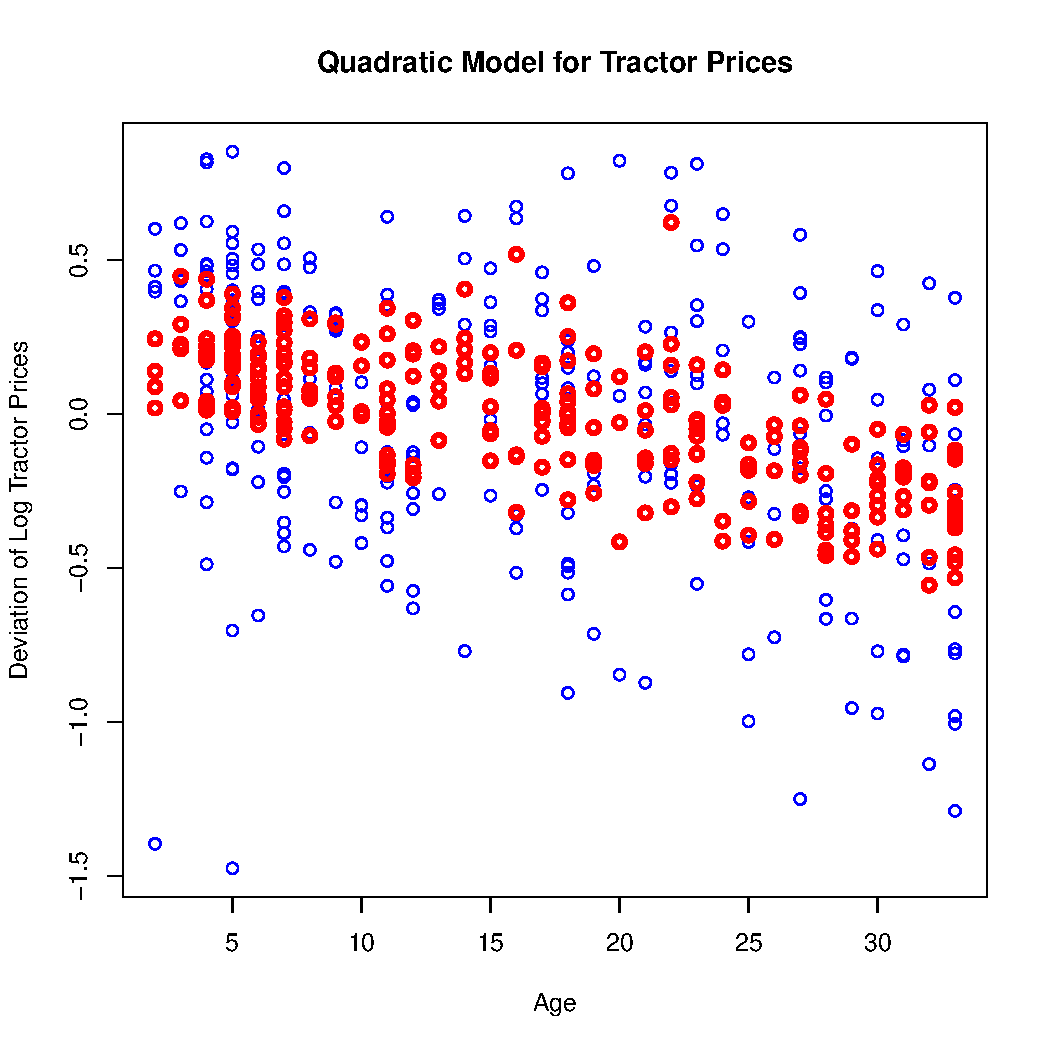
\includegraphics[scale = 0.5, keepaspectratio=true]{../Figures/dev_vs_age}
  \caption{Linear-Quadratic Model for Tractor Prices} \label{fig:dev_vs_age}
\end{figure}



\pagebreak
As a comparison, Figure \ref{fig:dev_vs_age_dev} 
augments the above by showing the plot against the 
residuals from the regression for age:
the ``excess age'' of a tractor compared to what would be 
expected given the other characteristics of the tractor. 
Notice that this time the fit follows a straight line,
since we have a single variable with no
quadratic transformation.

\begin{figure}[h!]
  \centering
  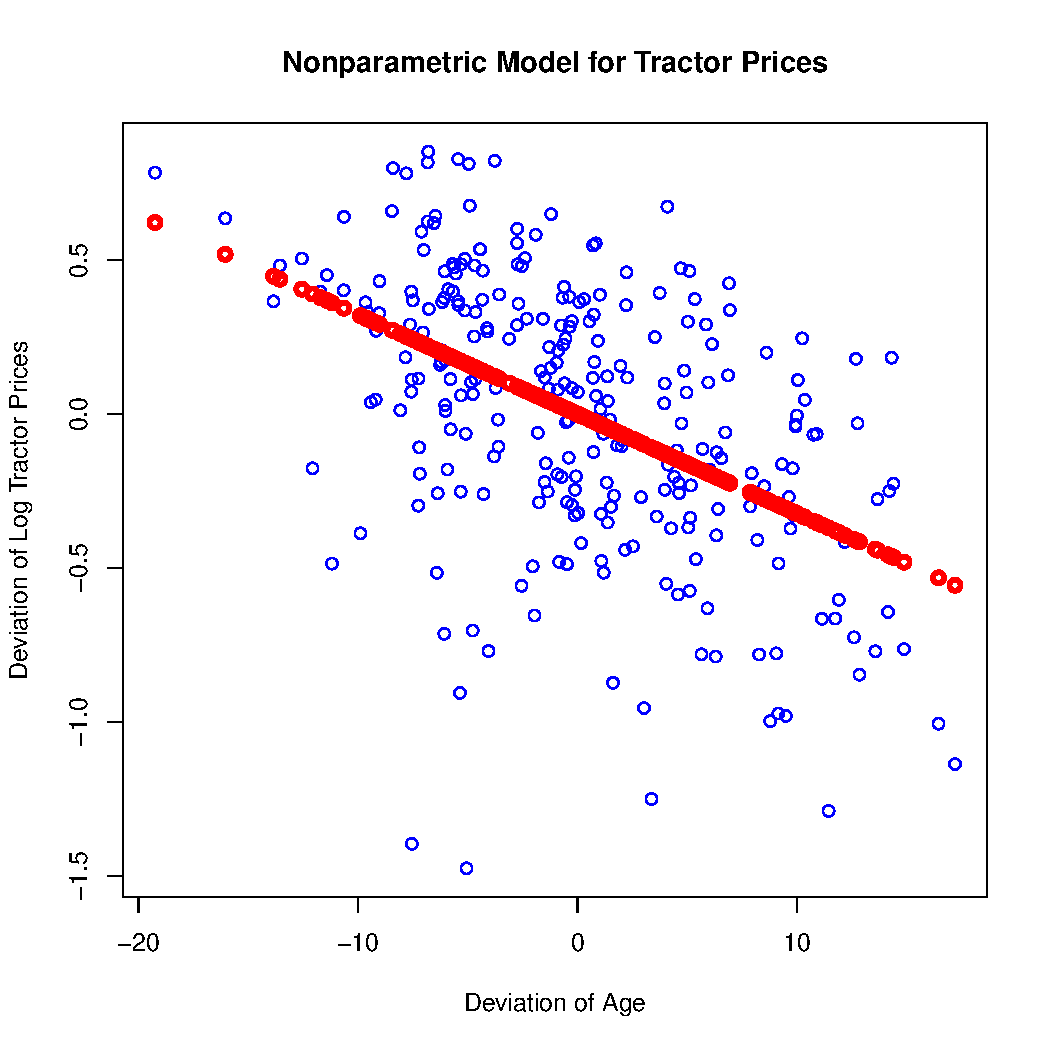
\includegraphics[scale = 0.5, keepaspectratio=true]{../Figures/dev_vs_age_dev}
  \caption{Linear-Quadratic Model for Tractor Prices: Excess Age} \label{fig:dev_vs_age_dev}
\end{figure}

\clearpage
Now consider a nonparametric specification for 
the relationship between prices and age.
Figure \ref{fig:dev_np_vs_age_dev} 
overlays the nonparametric estimate (shown in green) with the above in 
Figure \ref{fig:dev_vs_age_dev}.
The pattern has more variation in slope but 
closely follows the prediction from the linear model. 
Although the nonparametric estimate varies around the linear estimate,
it appears that the linear form
is a close enough approximation without the added complexity.
Next, I will explore the remaining continuous variable.


\begin{figure}[h!]
  \centering
  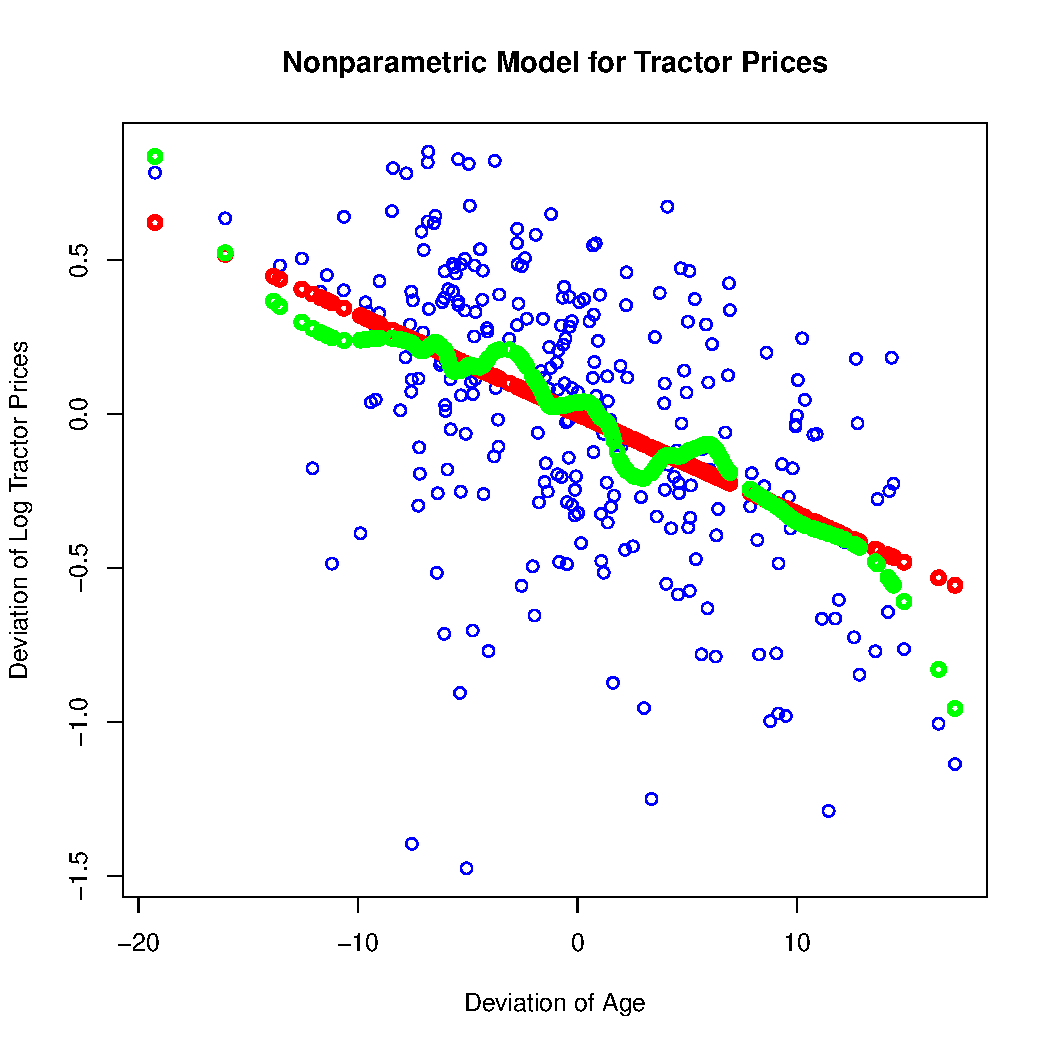
\includegraphics[scale = 0.5, keepaspectratio=true]{../Figures/dev_np_vs_age_dev}
  \caption{Nonparametric Model for Tractor Prices: Excess Age} \label{fig:dev_np_vs_age_dev}
\end{figure}





\clearpage
\subsection{Nonparametric Specification for Engine Hours}

As above, first conduct FWL regressions 
to reduce the problem to two dimensions. 
The models shown in
Table \ref{tab:reg_eng_fwl}
illustrate this possibility. 
Model 1 is the same original model in 
Table \ref{tab:reg_sq_horse}. 
Model 2 is a regression omitting the age variable. 
Model 3 is a regression to predict engine hours with the other explanatory variables in Model 2.
Finally, Model 4 shows the coefficient for engine hours
from a regression of the residuals of Model 2
on the residuals from Model 3. 
Notice that these coefficients match those in Model 1. 


\begin{table}
\begin{center}
\begin{tabular}{l c c c c}
\hline
 & Model 1 & Model 2 & Model 3 & Model 4 \\
\hline
(Intercept)         & $8.72792^{***}$  & $8.79201^{***}$  & $-1533.86328^{*}$ &                  \\
                    & $(0.10602)$      & $(0.10849)$      & $(671.52168)$     &                  \\
horsepower          & $0.01112^{***}$  & $0.01030^{***}$  & $19.70996^{**}$   &                  \\
                    & $(0.00107)$      & $(0.00108)$      & $(6.71576)$       &                  \\
squared\_horsepower & $-0.00001^{***}$ & $-0.00001^{***}$ & $-0.02012$        &                  \\
                    & $(0.00000)$      & $(0.00000)$      & $(0.01437)$       &                  \\
age                 & $-0.03233^{***}$ & $-0.04000^{***}$ & $183.63531^{***}$ &                  \\
                    & $(0.00358)$      & $(0.00322)$      & $(19.94860)$      &                  \\
enghours            & $-0.00004^{***}$ &                  &                   &                  \\
                    & $(0.00001)$      &                  &                   &                  \\
diesel              & $0.20350^{*}$    & $0.20799^{*}$    & $-107.43464$      &                  \\
                    & $(0.09805)$      & $(0.10130)$      & $(627.05359)$     &                  \\
fwd                 & $0.26539^{***}$  & $0.25967^{***}$  & $136.84215$       &                  \\
                    & $(0.05820)$      & $(0.06013)$      & $(372.16237)$     &                  \\
manual              & $-0.15015^{*}$   & $-0.15684^{*}$   & $160.15539$       &                  \\
                    & $(0.06189)$      & $(0.06393)$      & $(395.72599)$     &                  \\
johndeere           & $0.31872^{***}$  & $0.30410^{***}$  & $349.77262$       &                  \\
                    & $(0.07186)$      & $(0.07417)$      & $(459.11233)$     &                  \\
cab                 & $0.48345^{***}$  & $0.45588^{***}$  & $659.90018$       &                  \\
                    & $(0.07003)$      & $(0.07207)$      & $(446.07457)$     &                  \\
eng\_resid          &                  &                  &                   & $-0.00004^{***}$ \\
                    &                  &                  &                   & $(0.00001)$      \\
\hline
R$^2$               & $0.80591$        & $0.79200$        & $0.45819$         & $0.06689$        \\
Adj. R$^2$          & $0.79935$        & $0.78577$        & $0.44195$         & $0.06350$        \\
Num. obs.           & $276$            & $276$            & $276$             & $276$            \\
\hline
\multicolumn{5}{l}{\scriptsize{$^{***}p<0.001$; $^{**}p<0.01$; $^{*}p<0.05$}}
\end{tabular}
\caption{Linear Model for Engine Hours: FWL Regressions}
\label{tab:reg_eng_fwl}
\end{center}
\end{table}


\pagebreak 
To illustrate the fit of the model, 
Figure \ref{fig:dev_vs_eng} shows a scatter plot 
of the residual log prices on engine hours. 
The observations are shown in blue
and the fitted values are shown in red.
The variation in the fitted values results from the 
fact that it is not plotted against the transformed excess engine hours variable used in the regressions.
Still, the linear pattern is apparent
and appears to match the data. 

\begin{figure}[h!]
  \centering
  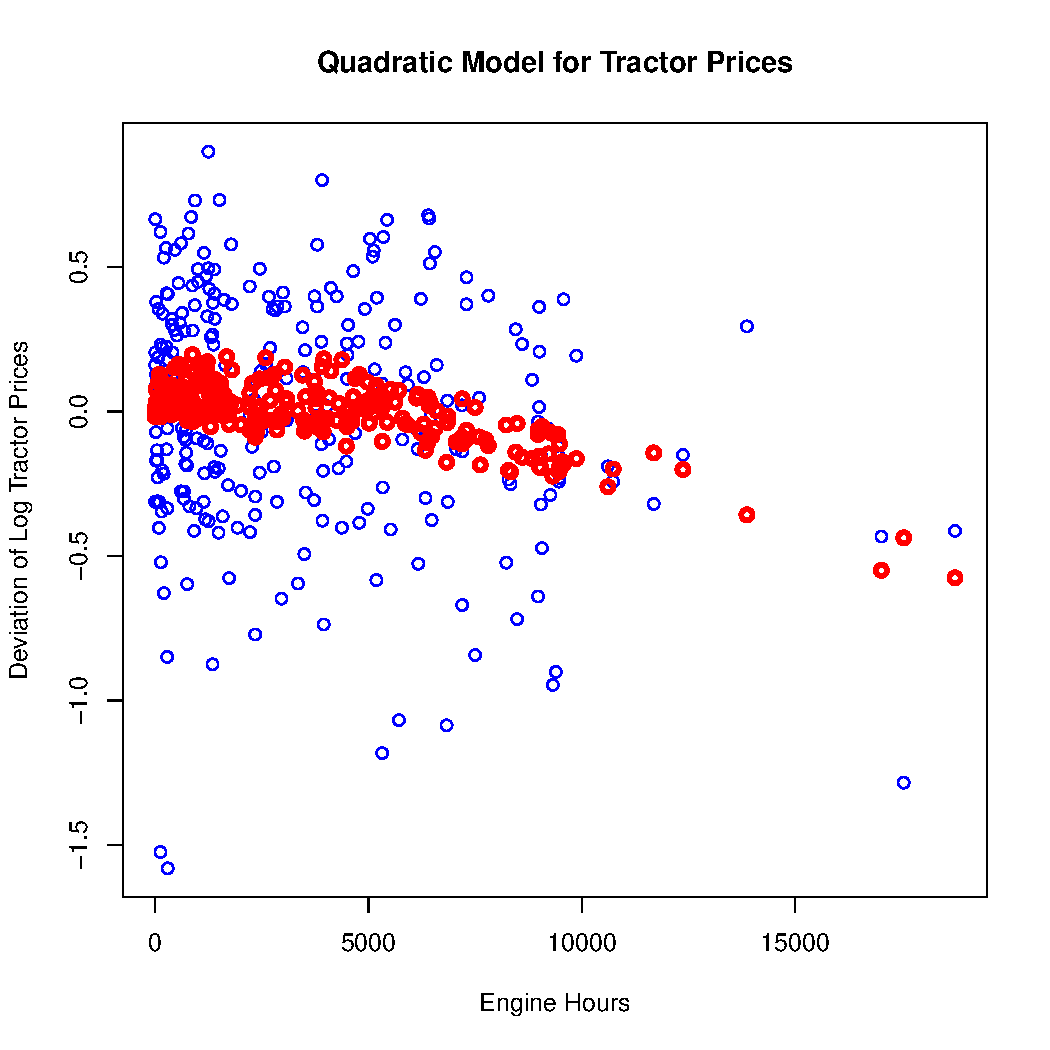
\includegraphics[scale = 0.5, keepaspectratio=true]{../Figures/dev_vs_eng}
  \caption{Linear-Quadratic Model for Tractor Prices} \label{fig:dev_vs_eng}
\end{figure}



\pagebreak
As a comparison, Figure \ref{fig:dev_np_vs_eng_dev} 
augments the above by showing the plot against the 
residuals from the regression for engine hours:
the ``excess engine hours'' of a tractor compared to what would be 
expected given the other characteristics of the tractor. 
As with age, the fit follows a straight line,
since we have a single variable with no
quadratic transformation.
% 
I move directly to the nonparametric specification for 
the relationship between prices and engine hours.
Figure \ref{fig:dev_np_vs_eng_dev} 
overlays the nonparametric estimate, shown in green. 
The pattern has more variation in slope but 
closely follows the prediction from the linear model. 
Although the nonparametric estimate varies around the linear estimate,
it appears that the linear form
is also a close enough approximation, 
just as was found for the age variable.


\begin{figure}[h!]
  \centering
  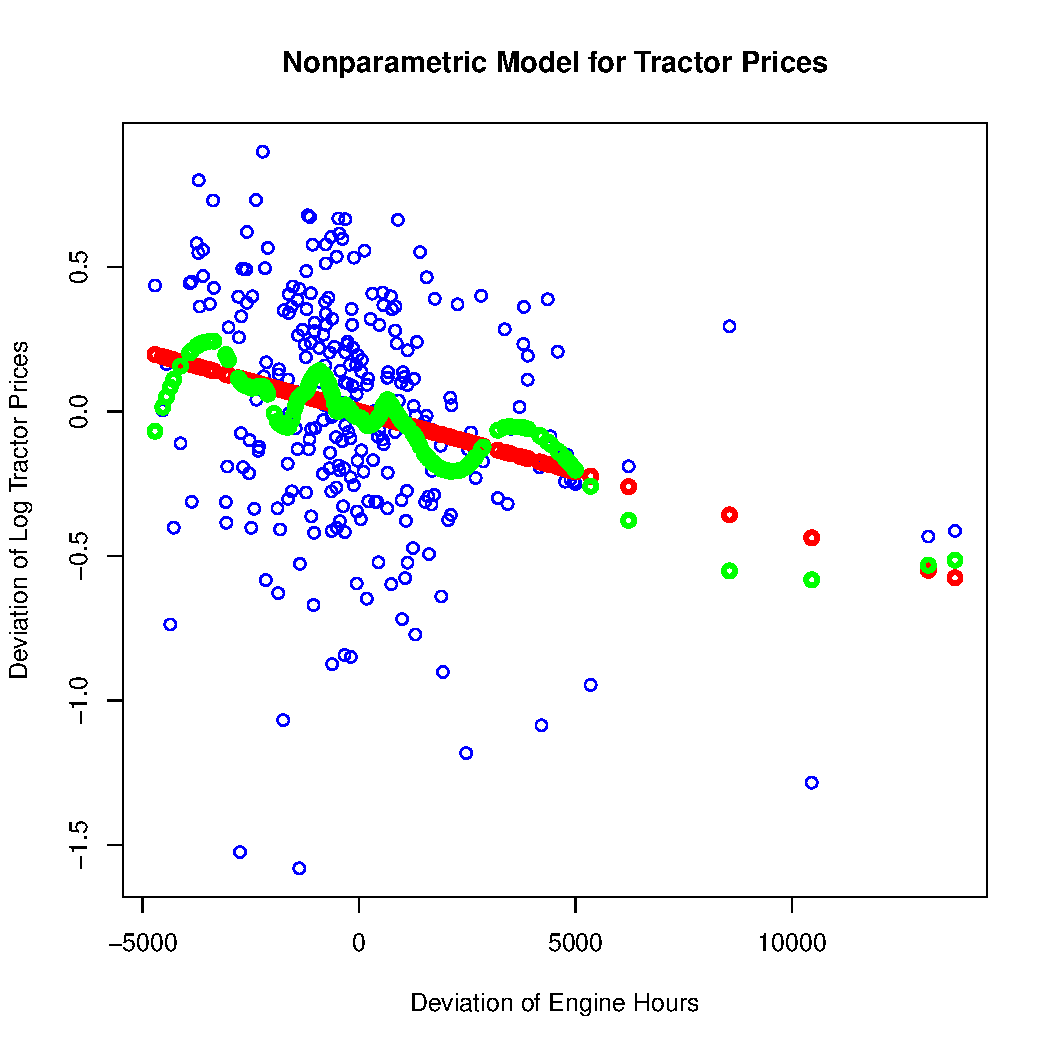
\includegraphics[scale = 0.5, keepaspectratio=true]{../Figures/dev_np_vs_eng_dev}
  \caption{Nonparametric Model for Tractor Prices: Excess Engine Hours} \label{fig:dev_np_vs_eng_dev}
\end{figure}

 

\pagebreak
\section{Semiparametric Estimates}

As I was building the above nonparametric models, 
I stored the predictions and will now use them as variables in 
linear models. 
Table \ref{tab:reg_semipar} 
shows the estimates from a set of models. 
Model 1 is the benchmark linear model in 
Table \ref{tab:reg_sq_horse}. 
Model 2 is a semi-parametric model
with a nonparametric fit on horsepower
substituted in for the horsepower variables.
Models 3 and 4 are semi-parametric models
with nonparametric fits on age and engine hours, respectively.
Model 5 is a maximally semiparametric model, 
with nonparametric fits for all continuous variables. 
For each of the single-variable semiparametric models, 
the coefficients are near one
and the fits are similar to the linear model. 
Even with maximal flexibility, the fit of Model 5
is not much better than the benchmark linear model. 
Across all models, the adjusted $\bar{R}^2$ values are all hovering around 0.80. 
All things considered, these are excellent models
and the linear model is sufficient.


\begin{table}
\begin{center}
\begin{tabular}{l c c c c c}
\hline
 & Model 1 & Model 2 & Model 3 & Model 4 & Model 5 \\
\hline
(Intercept)                 & $2.00999^{***}$ & $2.34926^{***}$ & $2.98091^{***}$  & $3.23438^{***}$ & $4.49531^{***}$  \\
                            & $(0.26125)$     & $(0.22596)$     & $(0.22704)$      & $(0.15261)$     & $(0.05897)$      \\
Width                       & $0.33575^{*}$   &                 & $0.92791^{***}$  & $0.03044$       &                  \\
                            & $(0.15622)$     &                 & $(0.12784)$      & $(0.14082)$     &                  \\
Diameter                    & $0.39567^{***}$ & $0.43144^{***}$ &                  & $0.33658^{***}$ &                  \\
                            & $(0.05076)$     & $(0.04150)$     &                  & $(0.04671)$     &                  \\
Density                     & $1.21296^{***}$ & $1.07566^{***}$ & $0.81613^{***}$  &                 &                  \\
                            & $(0.21948)$     & $(0.20093)$     & $(0.20645)$      &                 &                  \\
SealedYes                   & $0.62731^{***}$ & $0.61960^{***}$ & $0.70050^{***}$  & $0.56858^{***}$ & $0.69858^{***}$  \\
                            & $(0.08622)$     & $(0.08246)$     & $(0.08226)$      & $(0.08047)$     & $(0.07509)$      \\
MachinedYes                 & $0.64934^{***}$ & $0.58954^{***}$ & $0.71659^{***}$  & $0.65070^{***}$ & $0.61103^{***}$  \\
                            & $(0.08320)$     & $(0.07933)$     & $(0.07938)$      & $(0.07819)$     & $(0.07386)$      \\
made\_in\_USATRUE           & $0.74633^{***}$ & $0.77354^{***}$ & $0.79615^{***}$  & $0.70473^{***}$ & $0.79326^{***}$  \\
                            & $(0.09247)$     & $(0.08855)$     & $(0.08879)$      & $(0.08692)$     & $(0.08296)$      \\
SealedYes:made\_in\_USATRUE & $-0.29519^{**}$ & $-0.29826^{**}$ & $-0.33376^{***}$ & $-0.27253^{**}$ & $-0.31356^{***}$ \\
                            & $(0.10092)$     & $(0.09642)$     & $(0.09694)$      & $(0.09500)$     & $(0.09038)$      \\
width\_np                   &                 & $1.11995^{***}$ &                  &                 & $1.35512^{***}$  \\
                            &                 & $(0.21565)$     &                  &                 & $(0.20456)$      \\
diameter\_np                &                 &                 & $1.00650^{***}$  &                 & $1.00083^{***}$  \\
                            &                 &                 & $(0.10926)$      &                 & $(0.10411)$      \\
density\_np                 &                 &                 &                  & $1.03923^{***}$ & $0.76790^{***}$  \\
                            &                 &                 &                  & $(0.12864)$     & $(0.12582)$      \\
\hline
R$^2$                       & $0.74893$       & $0.76995$       & $0.76755$        & $0.77748$       & $0.79771$        \\
Adj. R$^2$                  & $0.74160$       & $0.76324$       & $0.76077$        & $0.77099$       & $0.79181$        \\
Num. obs.                   & $248$           & $248$           & $248$            & $248$           & $248$            \\
\hline
\multicolumn{6}{l}{\scriptsize{$^{***}p<0.001$; $^{**}p<0.01$; $^{*}p<0.05$}}
\end{tabular}
\caption{Semiparametric Models for Fly Reel Prices}
\label{tab:reg_semipar}
\end{center}
\end{table}






\pagebreak
\section{Generalized Additive Model}

\subsection{Linear Model}

As an example of the output from the GAM specification, 
I first estimated the model with no nonlinear terms, 
which is essentially a linear regression. 

\begin{verbatim}
Family: gaussian 
Link function: identity 

Formula:
log_saleprice ~ horsepower + squared_horsepower + age + enghours + 
    diesel + fwd + manual + johndeere + cab

Parametric coefficients:
                     Estimate Std. Error t value Pr(>|t|)    
(Intercept)         8.728e+00  1.060e-01  82.327  < 2e-16 ***
horsepower          1.112e-02  1.067e-03  10.423  < 2e-16 ***
squared_horsepower -1.404e-05  2.255e-06  -6.223 1.89e-09 ***
age                -3.233e-02  3.580e-03  -9.031  < 2e-16 ***
enghours           -4.178e-05  9.569e-06  -4.367 1.81e-05 ***
diesel              2.035e-01  9.805e-02   2.076   0.0389 *  
fwd                 2.654e-01  5.820e-02   4.560 7.82e-06 ***
manual             -1.502e-01  6.189e-02  -2.426   0.0159 *  
johndeere           3.187e-01  7.186e-02   4.435 1.35e-05 ***
cab                 4.834e-01  7.003e-02   6.903 3.72e-11 ***
---
Signif. codes:  0 �***� 0.001 �**� 0.01 �*� 0.05 �.� 0.1 � � 1


R-sq.(adj) =  0.799   Deviance explained = 80.6%
GCV = 0.16445  Scale est. = 0.15849   n = 276
\end{verbatim}

\pagebreak
\subsection{Semiparametric Model}


Further investigating the results of the full semiparametric specification
in Model 5 of Table \ref{tab:reg_semipar},
I estimated the model with all three continuous variables specified as nonparametric functions. 
The result was that 
almost all the variables---both linear and nonlinear---were 
statistically significant. 
The only exception was a loss in significance of the diesel indicator. 


\begin{verbatim}
Family: gaussian 
Link function: identity 

Formula:
log_saleprice ~ s(horsepower) + s(age) + s(enghours) + diesel + 
    fwd + manual + johndeere + cab

Parametric coefficients:
            Estimate Std. Error t value Pr(>|t|)    
(Intercept)  9.04516    0.09366  96.575  < 2e-16 ***
diesel       0.13440    0.09499   1.415  0.15830    
fwd          0.29899    0.05754   5.196 4.11e-07 ***
manual      -0.16938    0.05965  -2.839  0.00487 ** 
johndeere    0.33067    0.06890   4.799 2.68e-06 ***
cab          0.40439    0.07151   5.655 4.08e-08 ***
---
Signif. codes:  0 �***� 0.001 �**� 0.01 �*� 0.05 �.� 0.1 � � 1

Approximate significance of smooth terms:
                edf Ref.df     F  p-value    
s(horsepower) 4.387  5.321 44.89  < 2e-16 ***
s(age)        3.264  4.057 21.59  < 2e-16 ***
s(enghours)   1.000  1.000 23.39 2.64e-06 ***
---
Signif. codes:  0 �***� 0.001 �**� 0.01 �*� 0.05 �.� 0.1 � � 1

R-sq.(adj) =  0.819   Deviance explained = 82.8%
GCV = 0.15063  Scale est. = 0.14263   n = 276
\end{verbatim}

On the other hand, 
the adjusted R-squared has not increased very much, 
from 0.799 to 0.819 under this specification, 
which may not justify the added complexity of the model.
Perhaps more importantly, the coefficients on the 
linear terms are very similar across models, 
indicating that the models support similar conclusions relating to any business decision involving
the John Deere premium. 
With this second model, we have even more support for those conclusions
and are certain that the conclusions are not 
coincidental results of the
functional form decisions for previous models.


Perhaps as a middle ground, we can estimate a model with a 
nonparametric specification for the horsepower variable alone, 
since it seems to have a nonlinear relationship with value in either case. 
This retains most of the predictive value of the maximally 
semiparametric model and accommodates the 
nonlinear relationship with value of horsepower. 

\input{../Tables/reg_GAM_hp}



%%%%%%%%%%%%%%%%%%%%%%%%%%%%%%%%%%%%%%%%
\end{document}
%%%%%%%%%%%%%%%%%%%%%%%%%%%%%%%%%%%%%%%%


\pagebreak
%\documentclass[11pt]{paper}
%\usepackage{fullpage}
%\usepackage{palatino}
%\usepackage{amsfonts,amsmath,amssymb}
%% \usepackage{graphicx}
%
%\usepackage{listings}
%\usepackage{textcomp}
%\usepackage{color}
%
%\definecolor{dkgreen}{rgb}{0,0.6,0}
%\definecolor{gray}{rgb}{0.5,0.5,0.5}
%\definecolor{mauve}{rgb}{0.58,0,0.82}
%
%\lstset{frame=tb,
%  language=R,
%  aboveskip=3mm,
%  belowskip=3mm,
%  showstringspaces=false,
%  columns=flexible,
%  basicstyle={\small\ttfamily},
%  numbers=none,
%  numberstyle=\tiny\color{gray},
%  keywordstyle=\color{blue},
%  commentstyle=\color{dkgreen},
%  stringstyle=\color{mauve},
%  breaklines=true,
%  breakatwhitespace=true,
%  tabsize=3
%}
%
%
%
%\ifx\pdftexversion\undefined
%    \usepackage[dvips]{graphicx}
%\else
%    \usepackage[pdftex]{graphicx}
%    \usepackage{epstopdf}
%    \epstopdfsetup{suffix=}
%\fi
%
%\usepackage{subfig}
%
%
%% This allows pdflatex to print the curly quotes in the
%% significance codes in the output of the GAM.
%\UseRawInputEncoding
%
%\begin{document}

%%%%%%%%%%%%%%%%%%%%%%%%%%%%%%%%%%%%%%%%
% Problem Set 7
%%%%%%%%%%%%%%%%%%%%%%%%%%%%%%%%%%%%%%%%

%\pagestyle{empty}
%{\noindent\bf Spring 2021 \hfill Firstname M.~Lastname}
%\vskip 16pt
%\centerline{\bf University of Central Florida}
%\centerline{\bf College of Business}
%\vskip 16pt
%\centerline{\bf QMB 6911}
%\centerline{\bf Capstone Project in Business Analytics}
%\vskip 10pt
%\centerline{\bf Solutions:  Problem Set \#9}
%\vskip 32pt
%\noindent
%% 
%\section{Data Description}
%
%This analysis follows the script \texttt{Tractor\_Reg\_Model.R} to produce a more accurate model for used tractor prices with the data from \texttt{TRACTOR7.csv} in the \texttt{Data} folder. 
%The dataset includes the following variables.
%\begin{table}[h!]
%\begin{tabular}{l l l}
%
%$saleprice_i$ & = & the price paid for tractor $i$ in dollars \\
%% 
%$horsepower_i$ & = & the horsepower of tractor $i$ \\
%$age_i$ & = & the number of years since tractor $i$ was manufactured  \\
%$enghours_i$ & = & the number of hours of use recorded for tractor $i$  \\
%$diesel_i$ & = & an indicator of whether tractor $i$ runs on diesel fuel \\ %, $0$ otherwise \\
%$fwd_i$ & = & an indicator of whether tractor $i$ has four-wheel drive \\ %, $0$ otherwise \\
%$manual_i$ & = & an indicator of whether tractor $i$ has a manual transmission \\ %, $0$ otherwise \\
%$johndeere_i$ & = & an indicator of whether tractor $i$ is manufactured by John Deere \\ %, $0$ otherwise \\
%$cab_i$ & = & an indicator of whether tractor $i$ has an enclosed cab \\ %, $0$ otherwise \\
%% 
%$spring_i$ & = & an indicator of whether tractor $i$ was sold in April or May \\ %, $0$ otherwise \\
%$summer_i$ & = & an indicator of whether tractor $i$ was sold between June and September \\ %, $0$ otherwise \\
%$winter_i$ & = & an indicator of whether tractor $i$ was sold between December and March \\ %, $0$ otherwise \\
%
%\end{tabular}
%\end{table}
%%

I will revisit the recommended linear model
from Problem Set \#7, 
which included a quadratic specification for horsepower.
This allowed for an increasing relationship 
between price and horsepower, 
for tractors with low horsepower, 
but a decreasing relationship for the tractors with high horsepower. 
I augmented this model in the demonstration for 
Problem Set \#8 
by considering semiparametric specifications
within a Generalized Additive Model. 


Then I will further investigate this nonlinear relationship
by incorporating a nonlinear but parametric specification
for the value of horsepower. 
This parametric analysis will be performed
using the Box-Tidwell framework
to investigate whether the value of these characteristics
are best described with parametric nonlinear forms. 

%%%%%%%%%%%%%%%%%%%%%%%%%%%%%%%%%%%%%%%%
\clearpage
\section{Linear Regression Model}
%%%%%%%%%%%%%%%%%%%%%%%%%%%%%%%%%%%%%%%%

A natural staring point is the recommended linear model
from Problem Set \#7. 

\subsection{Quadratic Specification for Horsepower}

In the demo for Problem Set \#7, 
we considered the advice of
a used tractor dealer who reported that overpowered used tractors are hard to sell, since they consume more fuel. 
This implies that tractor prices often increase with horsepower, up to a point, but beyond that they decrease. 
To incorporate this advice, I created and included a variable for squared horsepower. 
A decreasing relationship for high values of horsepower
is characterized by 
a positive coefficient on the horsepower variable and
a negative coefficient on the squared horsepower variable. 

% 

\begin{table}
\begin{center}
\begin{tabular}{l c c c}
\hline
 & Model 1 & Model 2 & Model 3 \\
\hline
(Intercept)         & $8.60684^{***}$  & $8.72555^{***}$  & $8.72792^{***}$  \\
                    & $(0.11233)$      & $(0.11156)$      & $(0.10602)$      \\
horsepower          & $0.01504^{***}$  & $0.01115^{***}$  & $0.01112^{***}$  \\
                    & $(0.00097)$      & $(0.00107)$      & $(0.00107)$      \\
squared\_horsepower & $-0.00002^{***}$ & $-0.00001^{***}$ & $-0.00001^{***}$ \\
                    & $(0.00000)$      & $(0.00000)$      & $(0.00000)$      \\
age                 & $-0.03429^{***}$ & $-0.03206^{***}$ & $-0.03233^{***}$ \\
                    & $(0.00374)$      & $(0.00359)$      & $(0.00358)$      \\
enghours            & $-0.00004^{***}$ & $-0.00004^{***}$ & $-0.00004^{***}$ \\
                    & $(0.00001)$      & $(0.00001)$      & $(0.00001)$      \\
diesel              & $0.20070^{*}$    & $0.21453^{*}$    & $0.20350^{*}$    \\
                    & $(0.09975)$      & $(0.09854)$      & $(0.09805)$      \\
fwd                 & $0.31288^{***}$  & $0.27526^{***}$  & $0.26539^{***}$  \\
                    & $(0.06259)$      & $(0.05876)$      & $(0.05820)$      \\
johndeere           & $0.23842^{**}$   & $0.30972^{***}$  & $0.31872^{***}$  \\
                    & $(0.07705)$      & $(0.07236)$      & $(0.07186)$      \\
manual              &                  & $-0.15308^{*}$   & $-0.15015^{*}$   \\
                    &                  & $(0.06209)$      & $(0.06189)$      \\
cab                 &                  & $0.47786^{***}$  & $0.48345^{***}$  \\
                    &                  & $(0.07031)$      & $(0.07003)$      \\
spring              &                  & $-0.04892$       &                  \\
                    &                  & $(0.06506)$      &                  \\
summer              &                  & $-0.05729$       &                  \\
                    &                  & $(0.06379)$      &                  \\
winter              &                  & $0.04596$        &                  \\
                    &                  & $(0.07141)$      &                  \\
\hline
R$^2$               & $0.76838$        & $0.80761$        & $0.80591$        \\
Adj. R$^2$          & $0.76233$        & $0.79884$        & $0.79935$        \\
Num. obs.           & $276$            & $276$            & $276$            \\
\hline
\multicolumn{4}{l}{\scriptsize{$^{***}p<0.001$; $^{**}p<0.01$; $^{*}p<0.05$}}
\end{tabular}
\caption{Quadratic Models for Tractor Prices}
\label{tab:reg_sq_horse}
\end{center}
\end{table}

% 
The results of this regression specification are shown in 
Table \ref{tab:reg_sq_horse}. 
%
The squared horsepower variable has a coefficient of $-2.081e-05$, which is nearly ten times as large as the standard error of $2.199e-06$, which is very strong evidence against the null hypothesis of a positive or zero coefficient. 
I conclude that the log of the sale price does decline for large values of horsepower. 


With the squared horsepower variable, the $\bar{R}^2$ is $0.764$, indicating that it is a much stronger model than the others we considered. 
The $F$-statistic is large, indicating that it is a better candidate than the simple average log sale price. 
The new squared horsepower variable is statistically significant and the theory behind it is sound, since above a certain point, added horsepower may not improve performance but will cost more to operate. 
This new model is much improved over the previous models with a linear specification for horsepower.
Next, I will attempt to improve on this specification, 
as we did for Problem Set \#8. 





%%%%%%%%%%%%%%%%%%%%%%%%%%%%%%%%%%%%%%%%
\clearpage
\section{Nonlinear Specifications}
%%%%%%%%%%%%%%%%%%%%%%%%%%%%%%%%%%%%%%%%


% \clearpage
\subsection{Nonparametric Specification for Horsepower}


The specification in 
Table \ref{tab:reg_sq_horse}
assumes a quadratic functional form for
the relationship between price and horsepower. 
To consider the horsepower variable alone, 
while accounting for the effects of other variables, 
one can fit a nonparametric model to the residuals 
from a model of tractor prices, 
after regressing tractor prices on the other variables. 
This leaves only the variation in tractor prices that is not explained by the other variables. 
Going one step further, perform the same transformation to the horsepower variable:
take the residuals from a model of horsepower, 
after regressing horsepower on the other variables. 
This allows a model that would fit exactly the same as if it were estimated within a full model with all variables included. 

I first conducted FWL regressions 
to reduce the problem to two dimensions. 
The results are not shown here, 
since the comparison only verifies 
the conclusion of the FWL theorem. 


% \clearpage
To illustrate the fit of the model, 
\ref{fig:dev_vs_horse_dev} 
shows a scatter plot 
of the residual log prices on 
residuals from the regression for horsepower:
the ``excess horsepower'' compared to what would be 
expected given the other characteristics of a tractor. 
The observations are shown in blue
and the fitted values are shown in red.
The quadratic function is clear from this perspective, 
except that we observe variation in the fitted values results from the 
two-dimensional nature of the horsepower variable
when we consider the quadratic form.

I next considered a nonparametric specification for 
the relationship between prices and horsepower.
Figure \ref{fig:dev_np_vs_horse_dev} 
overlays the nonparametric estimate (shown in green) 
compared to the linear model.
The pattern has more variation in slope but 
closely follows the prediction from the quadratic model. 
So far, it appears that the quadratic form
is close enough.

\begin{figure}[h!]
  \centering
  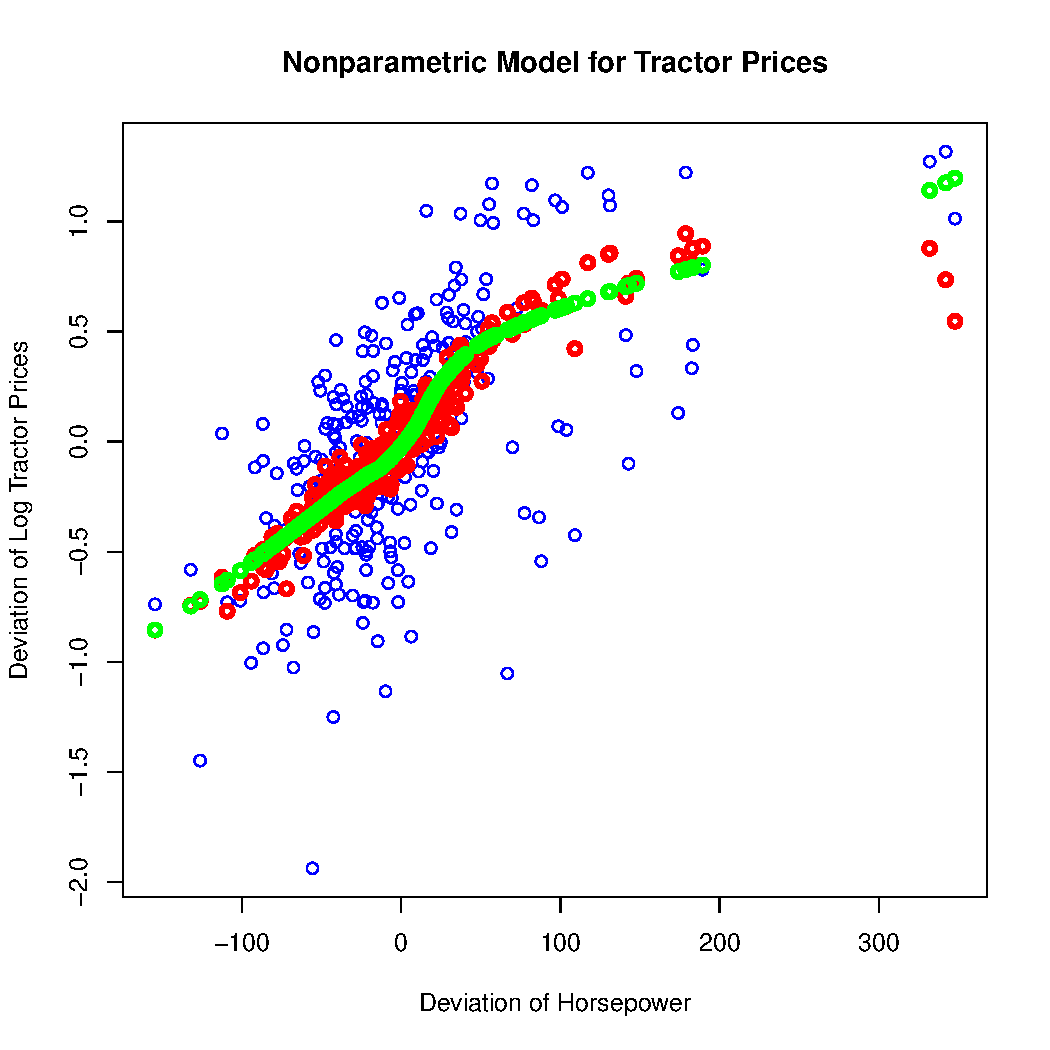
\includegraphics[scale = 0.5, keepaspectratio=true]{../Figures/dev_np_vs_horse_dev}
  \caption{Nonparametric Model for Tractor Prices: Excess Horsepower} \label{fig:dev_np_vs_horse_dev}
\end{figure}

 


\clearpage
\subsection{Nonparametric Specification for Age}

As above, first conduct FWL regressions 
to reduce the problem to two dimensions. 
% 
To illustrate the fit of the model, 
Figure \ref{fig:dev_np_vs_age_dev} 
shows a scatter plot 
of the residual log prices on 
the residuals from the regression for age:
the ``excess age'' of a tractor compared to what would be 
expected given the other characteristics of the tractor. 
% 
The observations are shown in blue
and the fitted values are shown in red.

Next we considered a nonparametric specification for 
the relationship between prices and age.
% 
Figure \ref{fig:dev_np_vs_age_dev} 
overlays the nonparametric estimate (shown in green) 
with the linear model.
The pattern has more variation in slope but 
closely follows the prediction from the linear model. 
Although the nonparametric estimate varies around the linear estimate,
it appears that the linear form
is a close enough approximation without the added complexity.
Next, I will revisit the remaining continuous variable.


\begin{figure}[h!]
  \centering
  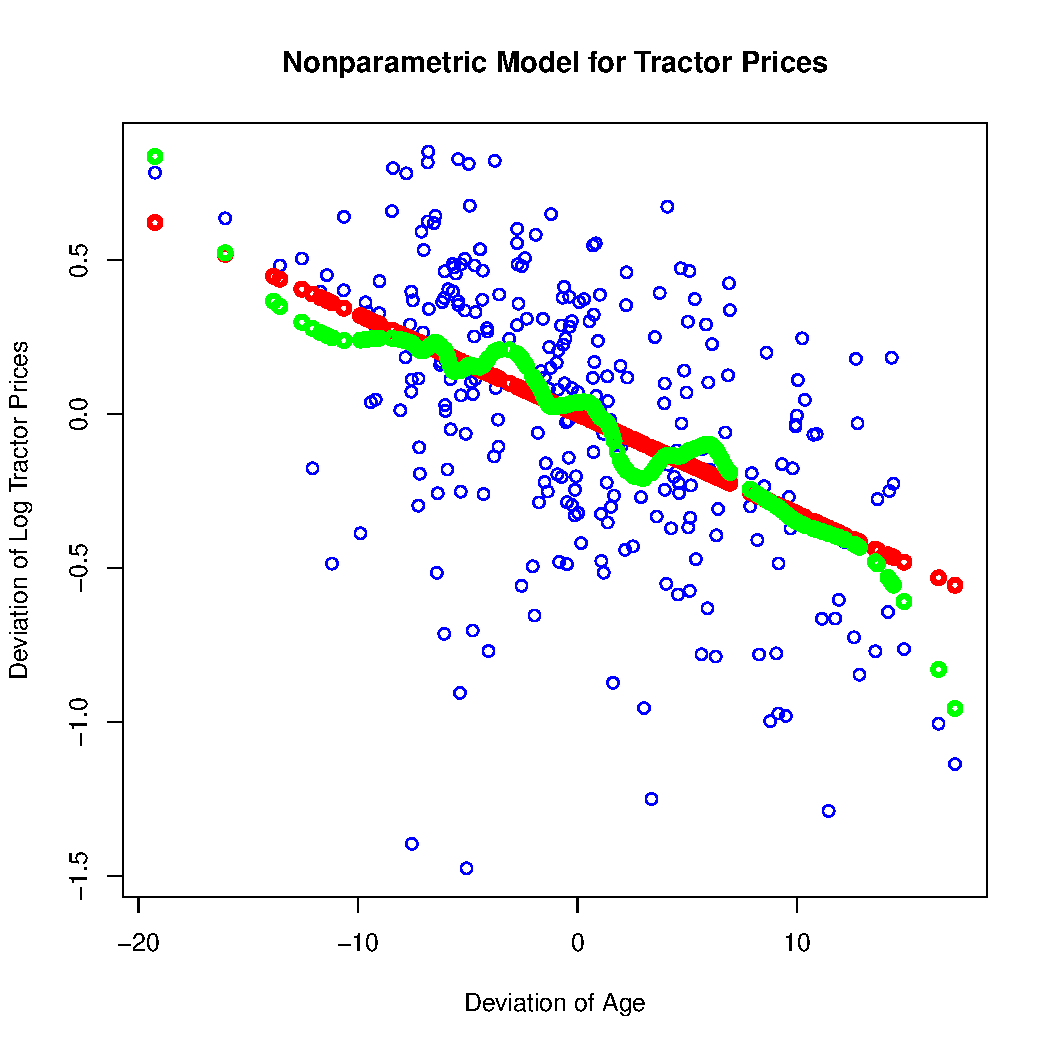
\includegraphics[scale = 0.5, keepaspectratio=true]{../Figures/dev_np_vs_age_dev}
  \caption{Nonparametric Model for Tractor Prices: Excess Age} \label{fig:dev_np_vs_age_dev}
\end{figure}





\clearpage
\subsection{Nonparametric Specification for Engine Hours}

As above, first conduct FWL regressions 
to reduce the problem to two dimensions. 
%
To illustrate the fit of the model, 
Figure \ref{fig:dev_np_vs_eng_dev}
shows a scatter plot 
of the residual log prices on 
residuals from the regression for engine hours:
the ``excess engine hours'' of a tractor compared to what would be 
expected given the other characteristics of the tractor. 
The observations are shown in blue
and the fitted values are shown in red.
As with age, the linear fit follows a straight line,
since we have a single variable with no
quadratic transformation.
% 
I moved directly to the nonparametric specification for 
the relationship between prices and engine hours.
Figure \ref{fig:dev_np_vs_eng_dev} 
overlays the nonparametric estimate, shown in green. 
The pattern has more variation in slope but 
closely follows the prediction from the linear model. 
Although the nonparametric estimate varies around the linear estimate,
it appears that the linear form
is also a close enough approximation, 
just as was found for the age variable.


\begin{figure}[h!]
  \centering
  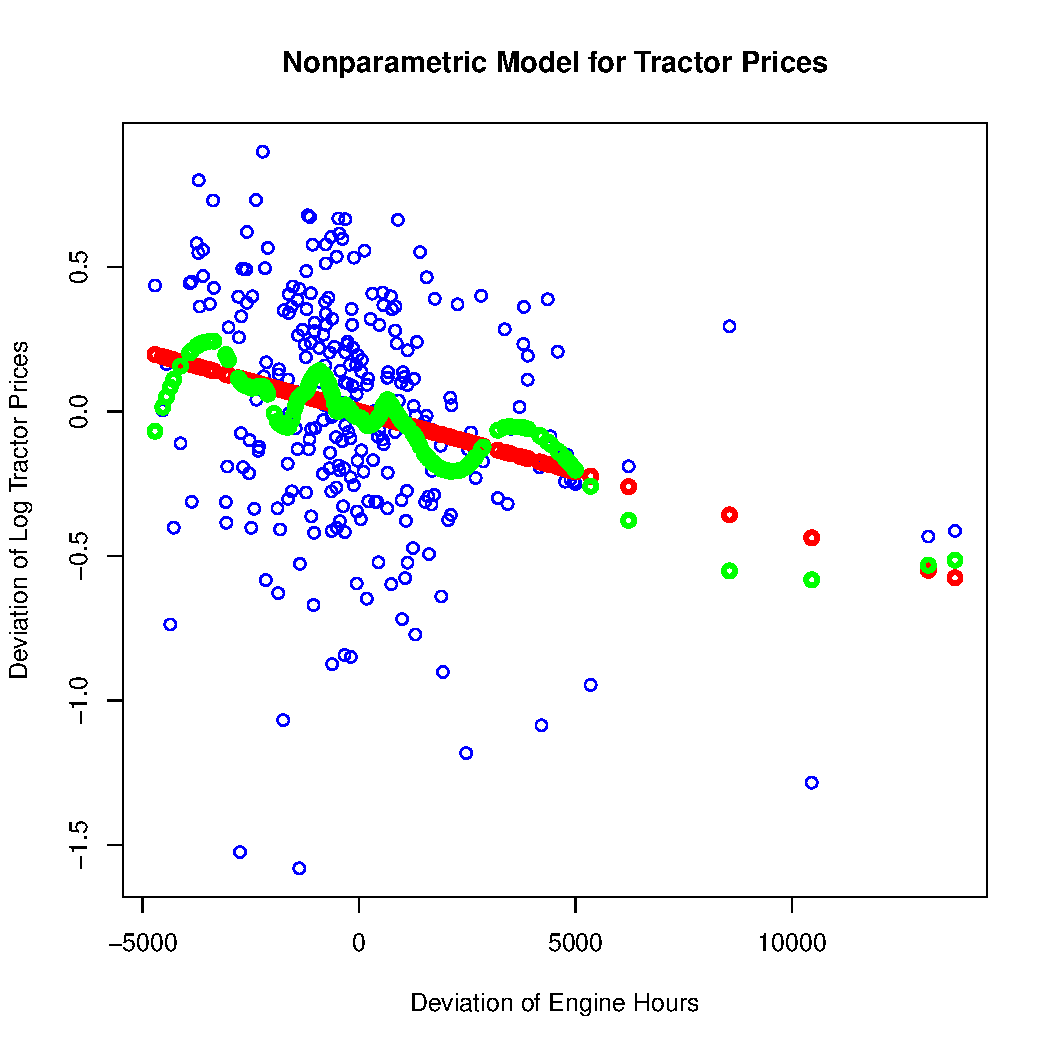
\includegraphics[scale = 0.5, keepaspectratio=true]{../Figures/dev_np_vs_eng_dev}
  \caption{Nonparametric Model for Tractor Prices: Excess Engine Hours} \label{fig:dev_np_vs_eng_dev}
\end{figure}

 

\pagebreak
\section{Semiparametric Estimates}

As I was building the above nonparametric models, 
I stored the predictions and will now use them as variables in 
linear models. 
Table \ref{tab:reg_semipar} 
shows the estimates from a set of models. 
Model 1 is the benchmark linear model in 
Table \ref{tab:reg_sq_horse}. 
Model 2 is a semi-parametric model
with a nonparametric fit on horsepower
substituted in for the horsepower variables.
Models 3 and 4 are semi-parametric models
with nonparametric fits on age and engine hours, respectively.
Model 5 is a maximally semiparametric model, 
with nonparametric fits for all continuous variables. 
For each of the single-variable semiparametric models, 
the coefficients are near one
and the fits are similar to the linear model. 
Even with maximal flexibility, the fit of Model 5
is not much better than the benchmark linear model. 
Across all models, the adjusted $\bar{R}^2$ values are all hovering around 0.80. 
All things considered, these are excellent models
and the linear model is sufficient.


\begin{table}
\begin{center}
\begin{tabular}{l c c c c c}
\hline
 & Model 1 & Model 2 & Model 3 & Model 4 & Model 5 \\
\hline
(Intercept)                 & $2.00999^{***}$ & $2.34926^{***}$ & $2.98091^{***}$  & $3.23438^{***}$ & $4.49531^{***}$  \\
                            & $(0.26125)$     & $(0.22596)$     & $(0.22704)$      & $(0.15261)$     & $(0.05897)$      \\
Width                       & $0.33575^{*}$   &                 & $0.92791^{***}$  & $0.03044$       &                  \\
                            & $(0.15622)$     &                 & $(0.12784)$      & $(0.14082)$     &                  \\
Diameter                    & $0.39567^{***}$ & $0.43144^{***}$ &                  & $0.33658^{***}$ &                  \\
                            & $(0.05076)$     & $(0.04150)$     &                  & $(0.04671)$     &                  \\
Density                     & $1.21296^{***}$ & $1.07566^{***}$ & $0.81613^{***}$  &                 &                  \\
                            & $(0.21948)$     & $(0.20093)$     & $(0.20645)$      &                 &                  \\
SealedYes                   & $0.62731^{***}$ & $0.61960^{***}$ & $0.70050^{***}$  & $0.56858^{***}$ & $0.69858^{***}$  \\
                            & $(0.08622)$     & $(0.08246)$     & $(0.08226)$      & $(0.08047)$     & $(0.07509)$      \\
MachinedYes                 & $0.64934^{***}$ & $0.58954^{***}$ & $0.71659^{***}$  & $0.65070^{***}$ & $0.61103^{***}$  \\
                            & $(0.08320)$     & $(0.07933)$     & $(0.07938)$      & $(0.07819)$     & $(0.07386)$      \\
made\_in\_USATRUE           & $0.74633^{***}$ & $0.77354^{***}$ & $0.79615^{***}$  & $0.70473^{***}$ & $0.79326^{***}$  \\
                            & $(0.09247)$     & $(0.08855)$     & $(0.08879)$      & $(0.08692)$     & $(0.08296)$      \\
SealedYes:made\_in\_USATRUE & $-0.29519^{**}$ & $-0.29826^{**}$ & $-0.33376^{***}$ & $-0.27253^{**}$ & $-0.31356^{***}$ \\
                            & $(0.10092)$     & $(0.09642)$     & $(0.09694)$      & $(0.09500)$     & $(0.09038)$      \\
width\_np                   &                 & $1.11995^{***}$ &                  &                 & $1.35512^{***}$  \\
                            &                 & $(0.21565)$     &                  &                 & $(0.20456)$      \\
diameter\_np                &                 &                 & $1.00650^{***}$  &                 & $1.00083^{***}$  \\
                            &                 &                 & $(0.10926)$      &                 & $(0.10411)$      \\
density\_np                 &                 &                 &                  & $1.03923^{***}$ & $0.76790^{***}$  \\
                            &                 &                 &                  & $(0.12864)$     & $(0.12582)$      \\
\hline
R$^2$                       & $0.74893$       & $0.76995$       & $0.76755$        & $0.77748$       & $0.79771$        \\
Adj. R$^2$                  & $0.74160$       & $0.76324$       & $0.76077$        & $0.77099$       & $0.79181$        \\
Num. obs.                   & $248$           & $248$           & $248$            & $248$           & $248$            \\
\hline
\multicolumn{6}{l}{\scriptsize{$^{***}p<0.001$; $^{**}p<0.01$; $^{*}p<0.05$}}
\end{tabular}
\caption{Semiparametric Models for Fly Reel Prices}
\label{tab:reg_semipar}
\end{center}
\end{table}






\pagebreak
\section{Generalized Additive Model}

\subsection{Linear Model}

As an example of the output from the GAM specification, 
I first estimated the model with no nonlinear terms, 
which is essentially a linear regression. 

\begin{verbatim}
Family: gaussian 
Link function: identity 

Formula:
log_saleprice ~ horsepower + squared_horsepower + age + enghours + 
    diesel + fwd + manual + johndeere + cab

Parametric coefficients:
                     Estimate Std. Error t value Pr(>|t|)    
(Intercept)         8.728e+00  1.060e-01  82.327  < 2e-16 ***
horsepower          1.112e-02  1.067e-03  10.423  < 2e-16 ***
squared_horsepower -1.404e-05  2.255e-06  -6.223 1.89e-09 ***
age                -3.233e-02  3.580e-03  -9.031  < 2e-16 ***
enghours           -4.178e-05  9.569e-06  -4.367 1.81e-05 ***
diesel              2.035e-01  9.805e-02   2.076   0.0389 *  
fwd                 2.654e-01  5.820e-02   4.560 7.82e-06 ***
manual             -1.502e-01  6.189e-02  -2.426   0.0159 *  
johndeere           3.187e-01  7.186e-02   4.435 1.35e-05 ***
cab                 4.834e-01  7.003e-02   6.903 3.72e-11 ***
---
Signif. codes:  0 �***� 0.001 �**� 0.01 �*� 0.05 �.� 0.1 � � 1


R-sq.(adj) =  0.799   Deviance explained = 80.6%
GCV = 0.16445  Scale est. = 0.15849   n = 276
\end{verbatim}

\pagebreak
\subsection{Semiparametric Model}


Further investigating the results of the full semiparametric specification
in Model 5 of Table \ref{tab:reg_semipar},
I estimated the model with all three continuous variables specified as nonparametric functions. 
The result was that 
almost all the variables---both linear and nonlinear---were 
statistically significant. 
The only exception was a loss in significance of the diesel indicator. 


\begin{verbatim}
Family: gaussian 
Link function: identity 

Formula:
log_saleprice ~ s(horsepower) + s(age) + s(enghours) + diesel + 
    fwd + manual + johndeere + cab

Parametric coefficients:
            Estimate Std. Error t value Pr(>|t|)    
(Intercept)  9.04516    0.09366  96.575  < 2e-16 ***
diesel       0.13440    0.09499   1.415  0.15830    
fwd          0.29899    0.05754   5.196 4.11e-07 ***
manual      -0.16938    0.05965  -2.839  0.00487 ** 
johndeere    0.33067    0.06890   4.799 2.68e-06 ***
cab          0.40439    0.07151   5.655 4.08e-08 ***
---
Signif. codes:  0 �***� 0.001 �**� 0.01 �*� 0.05 �.� 0.1 � � 1

Approximate significance of smooth terms:
                edf Ref.df     F  p-value    
s(horsepower) 4.387  5.321 44.89  < 2e-16 ***
s(age)        3.264  4.057 21.59  < 2e-16 ***
s(enghours)   1.000  1.000 23.39 2.64e-06 ***
---
Signif. codes:  0 �***� 0.001 �**� 0.01 �*� 0.05 �.� 0.1 � � 1

R-sq.(adj) =  0.819   Deviance explained = 82.8%
GCV = 0.15063  Scale est. = 0.14263   n = 276
\end{verbatim}

On the other hand, 
the adjusted R-squared has not increased very much, 
from 0.799 to 0.819 under this specification, 
which may not justify the added complexity of the model.
Perhaps more importantly, the coefficients on the 
linear terms are very similar across models, 
indicating that the models support similar conclusions relating to any business decision involving
the John Deere premium. 
With this second model, we have even more support for those conclusions
and are certain that the conclusions are not 
coincidental results of the
functional form decisions for previous models.


Perhaps as a middle ground, we can estimate a model with a 
nonparametric specification for the horsepower variable alone, 
since it seems to have a nonlinear relationship with value in either case. 
This retains most of the predictive value of the maximally 
semiparametric model and accommodates the 
nonlinear relationship with value of horsepower. 

\input{../Tables/reg_GAM_hp}


\pagebreak
\section{The Box--Tidwell Transformation}

The Box--Tidwell function tests for non-linear relationships
to the mean of the dependent variable.
The nonlinearity is in the form of an
exponential transformation in the form of the Box-Cox
transformation, except that the transformation is taken
on the explanatory variables.


\subsection{Transformation of Horsepower}


Performing the transformation on the horsepower variable
produces a modified form of the linear model.
This specification allows a single exponential
transformation on horsepower, rather than a quadratic form.

\begin{verbatim} MLE of lambda Score Statistic (z)  Pr(>|z|)    
       0.11437             -7.3864 1.509e-13 ***
---
Signif. codes:  0 �***� 0.001 �**� 0.01 �*� 0.05 �.� 0.1 � � 1

iterations =  5 
\end{verbatim}

The \textsf{R} output is the statistics for a test of nonlinearity:
that the exponent $\lambda$ in the Box--Tidwell transformation is zero.
%
The "\texttt{MLE of lambda}" statistic is the optimal exponent on horsepower.
Similar to the Box-Cox transformation,
with Box-Tidwell, the exponents are on the explanatory variables
and are all called lambda, in contrast
to the parameter $\tau$ in our class notes.
The exponent is significantly different from 0,
although it is a small positive value,
which suggests an increasing relationship
for the value of horsepower
with a slope that is sharply declining.
Next I consider the possibility of a changing relationship 
for the next continuous variable. 


\subsection{Transformation of Age}


\begin{verbatim} MLE of lambda Score Statistic (z) Pr(>|z|)
        0.9815              0.0421   0.9664

iterations =  3 
\end{verbatim}

This coefficient is effectively 1, which is more evidence of
a purely linear relationship between \texttt{log\_saleprice}
and age: the percentage depreciation rate is constant.
Next, I will consider the possibility of nonlinearity 
in depreciation from hours of use. 

\subsection{Transformation of Engine Hours}


\begin{verbatim} MLE of lambda Score Statistic (z) Pr(>|z|)
        1.3578             -0.9646   0.3348

iterations =  3 
\end{verbatim}

Although $\hat{\lambda}$ is not statistically significant,
this suggests a moderately increasing relationship
between the log of tractor prices and engine hours,
which means that tractors with high hours of use
depreciate more quickly with each additional hour of use.

Since a nonlinear relationship was detected with horsepower,
I will next estimate a model
with nonlinearity in all three continuous variables.


\subsection{Transformation of All Three Continuous Variables}


\begin{verbatim}           MLE of lambda Score Statistic (z)  Pr(>|z|)    
horsepower        0.1153             -7.1510 8.615e-13 ***
age               1.1183             -0.0489    0.9610    
enghours          1.1043             -0.5379    0.5907    
---
Signif. codes:  0 �***� 0.001 �**� 0.01 �*� 0.05 �.� 0.1 � � 1

iterations =  6 
\end{verbatim}


The performance is similar to the other models with
forms of nonlinearity for the value of horsepower.
Now consider the full set of such models in a table for a final comparison.


\pagebreak
\section{Final Comparison of Candidate Models}

I created one more variable \texttt{horsepower\_bt}
by raising horsepower to the optimal exponent 
$\hat{\lambda} = 0.1143693$. 
Then, I included this variable in the place of 
the horsepower variables a the linear regression model.
% 
Table \ref{tab:reg_sq_horse_sp_bt} collects the results
of the set of models from the three forms of nonlinearity.
Model 1 is the linear regression model with 
a quadratic form for horsepower. 
Model 2 is the semiparametric model with
a nonparametric form for horsepower. 
Model 3 has the same specification as the other two, 
except that the horsepower variable is transformed using the optimal
exponent for the Box-Tidwell transformation. 
% 
The last model has the highest R-squared
among the ones we have estimated.
Again, the differences are marginal, so the practical recommendation
is the model with the quadratic relationship for horsepower, 
which has a simpler interpretation.
In either case, we conclude that John Deere tractors are worth
approximately thirty percent more valuable
than an equivalent tractor of another brand. 


\begin{table}
\begin{center}
\begin{tabular}{l c c c}
\hline
 & Model 1 & Model 2 & Model 3 \\
\hline
(Intercept)         & $8.72792^{***}$  & $8.97543^{***}$  & $3.09024^{***}$  \\
                    & $(0.10602)$      & $(0.10479)$      & $(0.39174)$      \\
horsepower          & $0.01112^{***}$  &                  &                  \\
                    & $(0.00107)$      &                  &                  \\
squared\_horsepower & $-0.00001^{***}$ &                  &                  \\
                    & $(0.00000)$      &                  &                  \\
age                 & $-0.03233^{***}$ & $-0.03813^{***}$ & $-0.02927^{***}$ \\
                    & $(0.00358)$      & $(0.00360)$      & $(0.00345)$      \\
enghours            & $-0.00004^{***}$ & $0.00000$        & $-0.00005^{***}$ \\
                    & $(0.00001)$      & $(0.00001)$      & $(0.00001)$      \\
diesel              & $0.20350^{*}$    & $0.31981^{**}$   & $0.12070$        \\
                    & $(0.09805)$      & $(0.09872)$      & $(0.09500)$      \\
fwd                 & $0.26539^{***}$  & $0.39101^{***}$  & $0.32602^{***}$  \\
                    & $(0.05820)$      & $(0.05901)$      & $(0.05617)$      \\
manual              & $-0.15015^{*}$   & $-0.06208$       & $-0.20053^{**}$  \\
                    & $(0.06189)$      & $(0.06285)$      & $(0.06031)$      \\
johndeere           & $0.31872^{***}$  & $0.40778^{***}$  & $0.33386^{***}$  \\
                    & $(0.07186)$      & $(0.07313)$      & $(0.06967)$      \\
cab                 & $0.48345^{***}$  & $1.05513^{***}$  & $0.42139^{***}$  \\
                    & $(0.07003)$      & $(0.05806)$      & $(0.06768)$      \\
horsepower\_np      &                  & $0.96671^{***}$  &                  \\
                    &                  & $(0.06886)$      &                  \\
horsepower\_bt      &                  &                  & $3.99759^{***}$  \\
                    &                  &                  & $(0.25577)$      \\
\hline
R$^2$               & $0.80591$        & $0.79743$        & $0.81613$        \\
Adj. R$^2$          & $0.79935$        & $0.79136$        & $0.81062$        \\
Num. obs.           & $276$            & $276$            & $276$            \\
\hline
\multicolumn{4}{l}{\scriptsize{$^{***}p<0.001$; $^{**}p<0.01$; $^{*}p<0.05$}}
\end{tabular}
\caption{Alternate Models for Tractor Prices}
\label{tab:reg_sq_horse_sp_bt}
\end{center}
\end{table}




%%%%%%%%%%%%%%%%%%%%%%%%%%%%%%%%%%%%%%%%
% \end{document}
%%%%%%%%%%%%%%%%%%%%%%%%%%%%%%%%%%%%%%%%


\pagebreak
\documentclass[11pt]{paper}
\usepackage{fullpage}
\usepackage{palatino}
\usepackage{amsfonts,amsmath,amssymb}
% \usepackage{graphicx}

\usepackage{listings}
\usepackage{textcomp}
\usepackage{color}

\definecolor{dkgreen}{rgb}{0,0.6,0}
\definecolor{gray}{rgb}{0.5,0.5,0.5}
\definecolor{mauve}{rgb}{0.58,0,0.82}

\lstset{frame=tb,
  language=R,
  aboveskip=3mm,
  belowskip=3mm,
  showstringspaces=false,
  columns=flexible,
  basicstyle={\small\ttfamily},
  numbers=none,
  numberstyle=\tiny\color{gray},
  keywordstyle=\color{blue},
  commentstyle=\color{dkgreen},
  stringstyle=\color{mauve},
  breaklines=true,
  breakatwhitespace=true,
  tabsize=3
}



\ifx\pdftexversion\undefined
    \usepackage[dvips]{graphicx}
\else
    \usepackage[pdftex]{graphicx}
    \usepackage{epstopdf}
    \epstopdfsetup{suffix=}
\fi

\usepackage{subfig}


% This allows pdflatex to print the curly quotes in the
% significance codes in the output of the GAM.
\UseRawInputEncoding

\begin{document}

%%%%%%%%%%%%%%%%%%%%%%%%%%%%%%%%%%%%%%%%
% Problem Set 7
%%%%%%%%%%%%%%%%%%%%%%%%%%%%%%%%%%%%%%%%

\pagestyle{empty}
{\noindent\bf Spring 2021 \hfill Firstname M.~Lastname}
\vskip 16pt
\centerline{\bf University of Central Florida}
\centerline{\bf College of Business}
\vskip 16pt
\centerline{\bf QMB 6911}
\centerline{\bf Capstone Project in Business Analytics}
\vskip 10pt
\centerline{\bf Solutions:  Problem Set \#10}
\vskip 32pt
\noindent
% 
\section{Data Description}

This analysis follows the script \texttt{Tractor\_Reg\_Model.R} to produce a more accurate model for used tractor prices with the data from \texttt{TRACTOR7.csv} in the \texttt{Data} folder. 
The dataset includes the following variables.
\begin{table}[h!]
\begin{tabular}{l l l}

$saleprice_i$ & = & the price paid for tractor $i$ in dollars \\
% 
$horsepower_i$ & = & the horsepower of tractor $i$ \\
$age_i$ & = & the number of years since tractor $i$ was manufactured  \\
$enghours_i$ & = & the number of hours of use recorded for tractor $i$  \\
$diesel_i$ & = & an indicator of whether tractor $i$ runs on diesel fuel \\ %, $0$ otherwise \\
$fwd_i$ & = & an indicator of whether tractor $i$ has four-wheel drive \\ %, $0$ otherwise \\
$manual_i$ & = & an indicator of whether tractor $i$ has a manual transmission \\ %, $0$ otherwise \\
$johndeere_i$ & = & an indicator of whether tractor $i$ is manufactured by John Deere \\ %, $0$ otherwise \\
$cab_i$ & = & an indicator of whether tractor $i$ has an enclosed cab \\ %, $0$ otherwise \\
% 
$spring_i$ & = & an indicator of whether tractor $i$ was sold in April or May \\ %, $0$ otherwise \\
$summer_i$ & = & an indicator of whether tractor $i$ was sold between June and September \\ %, $0$ otherwise \\
$winter_i$ & = & an indicator of whether tractor $i$ was sold between December and March \\ %, $0$ otherwise \\

\end{tabular}
\end{table}
%

I will revisit the recommended linear model
from Problem Set \#7, 
which was supported in
Problem Sets \#8 and  \#9 
by considering other nonlinear specifications
within a Generalized Additive Model. 




Then I will further investigate this nonlinear relationship
by considering the issue of sample selection:
John Deere 
may produce 
tractors 
of specific qualities based on
their perceived value to typical 
John Deere 
customers, 
in ways that are not represented by the variables in the dataset.



%%%%%%%%%%%%%%%%%%%%%%%%%%%%%%%%%%%%%%%%
\clearpage
\section{Linear Regression Model}
%%%%%%%%%%%%%%%%%%%%%%%%%%%%%%%%%%%%%%%%

A natural staring point is the recommended linear model
from Problem Set \#7. 

\subsection{Quadratic Specification for Horsepower}

In the demo for Problem Set \#7, 
we considered the advice of
a used tractor dealer who reported that overpowered used tractors are hard to sell, since they consume more fuel. 
This implies that tractor prices often increase with horsepower, up to a point, but beyond that they decrease. 
To incorporate this advice, I created and included a variable for squared horsepower. 
A decreasing relationship for high values of horsepower
is characterized by 
a positive coefficient on the horsepower variable and
a negative coefficient on the squared horsepower variable. 

% 

\begin{table}
\begin{center}
\begin{tabular}{l c c c}
\hline
 & Model 1 & Model 2 & Model 3 \\
\hline
(Intercept)         & $8.60684^{***}$  & $8.72555^{***}$  & $8.72792^{***}$  \\
                    & $(0.11233)$      & $(0.11156)$      & $(0.10602)$      \\
horsepower          & $0.01504^{***}$  & $0.01115^{***}$  & $0.01112^{***}$  \\
                    & $(0.00097)$      & $(0.00107)$      & $(0.00107)$      \\
squared\_horsepower & $-0.00002^{***}$ & $-0.00001^{***}$ & $-0.00001^{***}$ \\
                    & $(0.00000)$      & $(0.00000)$      & $(0.00000)$      \\
age                 & $-0.03429^{***}$ & $-0.03206^{***}$ & $-0.03233^{***}$ \\
                    & $(0.00374)$      & $(0.00359)$      & $(0.00358)$      \\
enghours            & $-0.00004^{***}$ & $-0.00004^{***}$ & $-0.00004^{***}$ \\
                    & $(0.00001)$      & $(0.00001)$      & $(0.00001)$      \\
diesel              & $0.20070^{*}$    & $0.21453^{*}$    & $0.20350^{*}$    \\
                    & $(0.09975)$      & $(0.09854)$      & $(0.09805)$      \\
fwd                 & $0.31288^{***}$  & $0.27526^{***}$  & $0.26539^{***}$  \\
                    & $(0.06259)$      & $(0.05876)$      & $(0.05820)$      \\
johndeere           & $0.23842^{**}$   & $0.30972^{***}$  & $0.31872^{***}$  \\
                    & $(0.07705)$      & $(0.07236)$      & $(0.07186)$      \\
manual              &                  & $-0.15308^{*}$   & $-0.15015^{*}$   \\
                    &                  & $(0.06209)$      & $(0.06189)$      \\
cab                 &                  & $0.47786^{***}$  & $0.48345^{***}$  \\
                    &                  & $(0.07031)$      & $(0.07003)$      \\
spring              &                  & $-0.04892$       &                  \\
                    &                  & $(0.06506)$      &                  \\
summer              &                  & $-0.05729$       &                  \\
                    &                  & $(0.06379)$      &                  \\
winter              &                  & $0.04596$        &                  \\
                    &                  & $(0.07141)$      &                  \\
\hline
R$^2$               & $0.76838$        & $0.80761$        & $0.80591$        \\
Adj. R$^2$          & $0.76233$        & $0.79884$        & $0.79935$        \\
Num. obs.           & $276$            & $276$            & $276$            \\
\hline
\multicolumn{4}{l}{\scriptsize{$^{***}p<0.001$; $^{**}p<0.01$; $^{*}p<0.05$}}
\end{tabular}
\caption{Quadratic Models for Tractor Prices}
\label{tab:reg_sq_horse}
\end{center}
\end{table}

% 
The results of this regression specification are shown in 
Table \ref{tab:reg_sq_horse}. 
%
The squared horsepower variable has a coefficient of $-2.081e-05$, which is nearly ten times as large as the standard error of $2.199e-06$, which is very strong evidence against the null hypothesis of a positive or zero coefficient. 
I conclude that the log of the sale price does decline for large values of horsepower. 


With the squared horsepower variable, the $\bar{R}^2$ is $0.764$, indicating that it is a much stronger model than the others we considered. 
The $F$-statistic is large, indicating that it is a better candidate than the simple average log sale price. 
The new squared horsepower variable is statistically significant and the theory behind it is sound, since above a certain point, added horsepower may not improve performance but will cost more to operate. 
This new model is much improved over the previous models with a linear specification for horsepower.
Next, I will attempt to improve on this specification, 
using Tobit models for sample selection. 


%%%%%%%%%%%%%%%%%%%%%%%%%%%%%%%%%%%%%%%%
% \pagebreak
\subsubsection{Separate Models by Brand}
%%%%%%%%%%%%%%%%%%%%%%%%%%%%%%%%%%%%%%%%

To test for many possible differences in 
models by brand of tractor, 
Table \ref{tab:reg_johndeere}
shows the estimates for two separate models
by brand of tractor.
%
Model 1 shows the estimates for 
the full sample,
Model 2 shows the estimates from the full model for 
John Deere tractors
and Model 4 
represents all other brands. 
% 
Models 3 and 5 show the estimates from a reduced version of each model, 
in which all coefficients are statistically significant. 
% 
The coefficients appear similar across the two subsamples.
Notable differences include the statistical significance for 
the indicators for four-wheel drive, 
manual transmission and an enclosed cab. 
These features seem to change the value of 
other tractors, but perhaps these coefficients are not measured 
accurately for the small sample of 39 
John Deere tractors. 


\begin{table}
\begin{center}
\begin{tabular}{l c c c c c}
\hline
 & Model 1 & Model 2 & Model 3 & Model 4 & Model 5 \\
\hline
(Intercept)         & $8.72792^{***}$  & $8.86706^{***}$  & $9.03796^{***}$  & $8.77320^{***}$  & $8.90792^{***}$  \\
                    & $(0.10602)$      & $(0.22409)$      & $(0.16430)$      & $(0.12450)$      & $(0.08769)$      \\
horsepower          & $0.01112^{***}$  & $0.01502^{***}$  & $0.01580^{***}$  & $0.01032^{***}$  & $0.01057^{***}$  \\
                    & $(0.00107)$      & $(0.00250)$      & $(0.00223)$      & $(0.00119)$      & $(0.00119)$      \\
squared\_horsepower & $-0.00001^{***}$ & $-0.00002^{***}$ & $-0.00002^{***}$ & $-0.00001^{***}$ & $-0.00001^{***}$ \\
                    & $(0.00000)$      & $(0.00000)$      & $(0.00000)$      & $(0.00000)$      & $(0.00000)$      \\
age                 & $-0.03233^{***}$ & $-0.03038^{**}$  & $-0.03295^{***}$ & $-0.03164^{***}$ & $-0.03283^{***}$ \\
                    & $(0.00358)$      & $(0.00914)$      & $(0.00738)$      & $(0.00399)$      & $(0.00392)$      \\
enghours            & $-0.00004^{***}$ & $-0.00006^{*}$   & $-0.00006^{**}$  & $-0.00004^{***}$ & $-0.00004^{***}$ \\
                    & $(0.00001)$      & $(0.00002)$      & $(0.00002)$      & $(0.00001)$      & $(0.00001)$      \\
diesel              & $0.20350^{*}$    & $0.08485$        &                  & $0.18218$        &                  \\
                    & $(0.09805)$      & $(0.18242)$      &                  & $(0.11984)$      &                  \\
fwd                 & $0.26539^{***}$  & $0.12882$        &                  & $0.29072^{***}$  & $0.30003^{***}$  \\
                    & $(0.05820)$      & $(0.15529)$      &                  & $(0.06308)$      & $(0.06296)$      \\
manual              & $-0.15015^{*}$   & $0.06749$        &                  & $-0.17919^{**}$  & $-0.14668^{*}$   \\
                    & $(0.06189)$      & $(0.17288)$      &                  & $(0.06743)$      & $(0.06413)$      \\
johndeere           & $0.31872^{***}$  &                  &                  &                  &                  \\
                    & $(0.07186)$      &                  &                  &                  &                  \\
cab                 & $0.48345^{***}$  & $0.32344$        & $0.38517^{*}$    & $0.51732^{***}$  & $0.52756^{***}$  \\
                    & $(0.07003)$      & $(0.17555)$      & $(0.16365)$      & $(0.07696)$      & $(0.07688)$      \\
\hline
R$^2$               & $0.80591$        & $0.91993$        & $0.91606$        & $0.77992$        & $0.77769$        \\
Adj. R$^2$          & $0.79935$        & $0.89858$        & $0.90334$        & $0.77220$        & $0.77090$        \\
Num. obs.           & $276$            & $39$             & $39$             & $237$            & $237$            \\
\hline
\multicolumn{6}{l}{\scriptsize{$^{***}p<0.001$; $^{**}p<0.01$; $^{*}p<0.05$}}
\end{tabular}
\caption{Separate Models by Brand}
\label{tab:reg_johndeere}
\end{center}
\end{table}


We can also test for all of the differences at the same time
by using an $F$-test. 
In this case, the full, unrestricted model has $K = 2\times9 = 18$ parameters, one for each variable in two models. 
The test that all of the coefficients are the same has $M = 9 - 1 = 8$
restrictions. 
The one restriction fewer accounts for the John Deere indicator
in the full model, 
which allows for two separate intercepts. 
% 
The $F$-statistic has a value of 

$$ 
\frac{(RSS_M - RSS)/M}{RSS/(N - K - 1)} = \frac{(42.15882 - 41.1432)/3}{41.1432/263} = 0.7929991. 
$$

This is also a very low value for the $F$-statistic. 
There is no evidence to reject the null that all 
coefficients are equal across both samples 
and conclude that the John Deere indicator
should be the only brand difference left in the model. 



%%%%%%%%%%%%%%%%%%%%%%%%%%%%%%%%%%%%%%%%
\clearpage
\section{Sample Selection}
%%%%%%%%%%%%%%%%%%%%%%%%%%%%%%%%%%%%%%%%


% \clearpage
\subsection{Predicting the Selection into Samples}


The specification in 
Table \ref{tab:reg_sq_horse}
assumes a quadratic functional form for
the relationship between price and horsepower, 
without selecting into samples by brand.
% 
To investigate this relationship further, 
consider the set of variables that are related to
whether or not John Deere makes a tractor
with the characteristics observed in the dataset. 


\begin{table}
\begin{center}
\begin{tabular}{l c c}
\hline
 & Model 1 & Model 2 \\
\hline
(Intercept)    & $-3.46545$       & $3.38980^{**}$   \\
               & $(159.27332)$    & $(1.06142)$      \\
Weight         & $0.11330$        & $0.13348^{*}$    \\
               & $(0.19412)$      & $(0.05711)$      \\
Diameter       & $-0.08526$       &                  \\
               & $(0.86262)$      &                  \\
Width          & $-0.71463$       & $-2.45931^{**}$  \\
               & $(1.68668)$      & $(0.81177)$      \\
Volume         & $-0.03294$       &                  \\
               & $(0.09631)$      &                  \\
Density        & $-2.19723$       & $-2.02613^{*}$   \\
               & $(2.46062)$      & $(0.98455)$      \\
SealedYes      & $-1.23411^{***}$ & $-0.68650^{***}$ \\
               & $(0.23449)$      & $(0.18639)$      \\
MachinedYes    & $6.58401$        &                  \\
               & $(159.21535)$    &                  \\
\hline
AIC            & $267.46344$      & $328.68383$      \\
BIC            & $295.57087$      & $346.25098$      \\
Log Likelihood & $-125.73172$     & $-159.34192$     \\
Deviance       & $251.46344$      & $318.68383$      \\
Num. obs.      & $248$            & $248$            \\
\hline
\multicolumn{3}{l}{\scriptsize{$^{***}p<0.001$; $^{**}p<0.01$; $^{*}p<0.05$}}
\end{tabular}
\caption{Probit Models for Country-of-Manufacture Selection of Fly Reels}
\label{tab:reg_probit}
\end{center}
\end{table}


Table \ref{tab:reg_probit} 
shows the estimates for a probit model to predict the selection
into samples by brand name.
% 
Model 1 in Table \ref{tab:reg_probit} 
shows a preliminary probit model to predict the selection indicator,
with all the other explanatory variables in the model.
John Deere tractors are more likely to be gasoline-powered,
have manual transmissions, and less likely to have an enclosed cab.
% 
Model 2 shows the result of a variable-reduction exercise
to eliminate variables that are not statistically significant.
These estimates provide a concise but useful model to
indicate the tractor designs that would be favored by John Deere
engineers and customers.
This model is used to specify the selection equation
of the sample selection estimates investigated next. 
 
% \clearpage
\subsection{Estimating a Sample Selection Model}

In this section, I will make a valiant attempt to fit 
a sample selection model to the tractor sales data. 
This exercise is useful because it illustrates a level of difficulty
that is often encountered when conducting maximum likelihood estimation, 
or any for of estimation that involves numeric optimization
with a complex objective function. 
% 

In contrast, in the sections above, I applied linear regression
to separate samples by brand of tractor. 
I also fit a probit model to predict the brand of a tractor 
based on its characteristics. 
In each of these cases, the estimation run much more smoothly. 
With linear regression, the parameter estimates are obtained 
from calculation following a closed-form analytical solution obtained by calculus. 
This calculation is well-defined, except in very well understood cases
that can be identified beforehand. 
Similarly, in the case of the probit model, the likelihood function is well-behaved, with a convex shape like a smooth hill. 

When one fits a much more complex model, 
such as the Tobit type 5 switching model, 
the situation is different. 
Not only are we estimating parameters for three equations at once---%
one selection equation into two brand groups and two observation equations for those groups---%
the likelihood function can have multiple optima
or, as we will see, will often encounter regions of the parameter space in which the required calculations are undefined. 



% \clearpage
\subsubsection{Sample Selection Model 1: Full Model}

For a first model, I use the entire set of variables
for both observation equations, for John Deere and other brands.
I specify the selection equation with the variables above
from the probit model.


\begin{lstlisting}[language=R]
tobit_5_sel_1 <-
   selection(selection = johndeere ~
                diesel + manual + cab,
             outcome = list(log_price_other ~
                               horsepower +
                               squared_horsepower +
                               age +
                               enghours +
                               diesel +
                               fwd +
                               manual +
                               cab,
                            log_price_JD ~
                               horsepower +
                               squared_horsepower +
                               age +
                               enghours +
                               diesel +
                               fwd +
                               manual +
                               cab),
             iterlim = 20,
             # method = '2step',
             data = tractor_sales)
\end{lstlisting}


Note that this printed some warning messages:


\begin{lstlisting}[language=R]
Warning messages:
1: In heckit5fit(selection, as.formula(formula1), as.formula(formula2),  :
 Inverse Mills Ratio is virtually multicollinear to the rest of explanatory
 variables in the outcome equation 1
2: In heckit5fit(selection, as.formula(formula1), as.formula(formula2),  :
 Inverse Mills Ratio is virtually multicollinear to the rest of explanatory
 variables in the outcome equation 2
\end{lstlisting}

This suggests much overlap between the two models.
This is a risk of starting with too rich a model. 
Inspecting the model summary gives the following result.


\begin{lstlisting}[language=R]
R> summary(tobit_5_sel_1)
--------------------------------------------
Tobit 5 model (switching regression model)
Maximum Likelihood estimation
Newton-Raphson maximisation, 12 iterations
Return code 3: Last step could not find a value above the current.
Boundary of parameter space?  
Consider switching to a more robust optimisation method temporarily.
Log-Likelihood: -268.2932 
276 observations: 237 selection 1 (0) and 39 selection 2 (1)
26 free parameters (df = 250)
Probit selection equation:
            Estimate Std. Error t value Pr(>|t|)
(Intercept)  -0.4064        Inf       0        1
diesel       -0.9974        Inf       0        1
manual        0.5731        Inf       0        1
cab          -0.5105        Inf       0        1
Outcome equation 1:
                     Estimate Std. Error t value Pr(>|t|)
(Intercept)         8.373e+00        Inf       0        1
horsepower          8.717e-03        Inf       0        1
squared_horsepower -1.024e-05        Inf       0        1
age                -2.403e-02        Inf       0        1
enghours           -2.961e-05        Inf       0        1
diesel              4.411e-01        Inf       0        1
fwd                 3.966e-01        Inf       0        1
manual             -3.577e-01        Inf       0        1
cab                 6.171e-01        Inf       0        1
Outcome equation 2:
                     Estimate Std. Error t value Pr(>|t|)
(Intercept)         9.245e+00        Inf       0        1
horsepower          1.838e-02        Inf       0        1
squared_horsepower -2.557e-05        Inf       0        1
age                -1.895e-02        Inf       0        1
enghours           -7.279e-05        Inf       0        1
diesel              6.111e-01        Inf       0        1
fwd                 3.582e-01        Inf       0        1
manual             -1.247e-01        Inf       0        1
cab                 4.143e-01        Inf       0        1
   Error terms:
       Estimate Std. Error t value Pr(>|t|)
sigma1   0.5428        Inf       0        1
sigma2   0.7614        Inf       0        1
rho1    -0.9598        Inf       0        1
rho2    -0.9999        Inf       0        1
--------------------------------------------
\end{lstlisting}

The messages surrounding the optimization suggest a problematic
search for the parameter values. 
Also, the standard errors could not be calculated.
Furthermore, when I toggled the \texttt{method = '2step'} commented line, 
the situation did not improve, aside from returning the results from separate models as in the analysis above. 
% 
Again, problems such as these are often encountered when starting with too rich a model. 
Perhaps a less ambitious model is a better starting point. 



\subsubsection{Sample Selection Model 2: Reduced Model from Separate Estimation}

Instead of starting with a ``big-to-small'' approach,
I reconsider the best models for each tractor brand group 
that were recommended above.
I specify the selection equation with the variables above
from the probit model.
For this refined model, I use the set of variables
for separate observation equations,
to match the reduced models from separate linear regressions
for John Deere and other tractor brands.


\begin{lstlisting}[language=R]
tobit_5_sel_2 <-
   selection(selection = johndeere ~
                diesel + manual + cab,
             outcome = list(log_price_other ~
                               horsepower +
                               squared_horsepower +
                               age +
                               enghours +
                               # diesel +
                               fwd +
                               manual +
                               cab,
                            log_price_JD ~
                               horsepower +
                               squared_horsepower +
                               age +
                               enghours +
                               # diesel +
                               # fwd +
                               # manual +
                               cab),
             iterlim = 20,
             # method = '2step',
             data = tractor_sales)

\end{lstlisting}

Although there were no error messages this time, 
the results were similarly disappointing. 
Ideally, this estimation method produces standard errors in the above summary
but I can inspect the results from the separate models for each sample.
For instance, from the linear model for other brands, 
after using the \texttt{method = '2step'} argument, I obtain the following.

\begin{lstlisting}[language=R]
> summary(tobit_5_sel_2$lm1)

Call:
lm(formula = YO1 ~ -1 + XO1)

Residuals:
     Min       1Q   Median       3Q      Max 
-1.65134 -0.20946  0.04333  0.27656  0.70671 

Coefficients:
                        Estimate Std. Error t value Pr(>|t|)    
XO1(Intercept)         8.973e+00  1.142e-01  78.588  < 2e-16 ***
XO1horsepower          1.046e-02  1.193e-03   8.764 4.38e-16 ***
XO1squared_horsepower -1.311e-05  2.559e-06  -5.122 6.44e-07 ***
XO1age                -3.210e-02  4.004e-03  -8.016 5.66e-14 ***
XO1enghours           -3.861e-05  1.077e-05  -3.586 0.000411 ***
XO1fwd                 2.965e-01  6.311e-02   4.699 4.53e-06 ***
XO1manual             -1.107e-01  7.570e-02  -1.462 0.145173    
XO1cab                 4.843e-01  9.078e-02   5.335 2.30e-07 ***
XO1invMillsRatio      -2.694e-01  3.005e-01  -0.897 0.370771    
---
Signif. codes:  0 ‘***’ 0.001 ‘**’ 0.01 ‘*’ 0.05 ‘.’ 0.1 ‘ ’ 1

Residual standard error: 0.406 on 228 degrees of freedom
Multiple R-squared:  0.9983,	Adjusted R-squared:  0.9982 
F-statistic: 1.447e+04 on 9 and 228 DF,  p-value: < 2.2e-16
\end{lstlisting}

One should be cautious in interpreting these results, 
since the standard errors are underestimated, 
since this linear model does not account for the uncertainty
in the switching component of the sample selection model.
Still, this suggests that I can remove the \texttt{manual} indicator.
A similar investigation of the \texttt{tobit\_5\_sel\_2\$lm2} model object
suggests that the \texttt{cab} variable can be removed as well. 

\subsubsection{Sample Selection Model 3: Reduced Model}

I estimate a model that is the same as the last in all ways, 
except that the \texttt{manual} variable was removed from the first observation equation (other tractors)
and the \texttt{cab} variable from the second (John Deere) equation. 

\begin{lstlisting}[language=R]
tobit_5_sel_3 <-
   selection(selection = johndeere ~
                diesel + manual + cab,
             outcome = list(log_price_other ~
                               horsepower +
                               squared_horsepower +
                               age +
                               enghours +
                               # diesel +
                               fwd +
                               # manual +
                               cab,
                            log_price_JD ~
                               horsepower +
                               squared_horsepower +
                               age # +
                               # enghours # +
                               # diesel +
                               # fwd +
                               # manual +
                               # cab
                            ),
             iterlim = 20,
             method = '2step',
             data = tractor_sales)

\end{lstlisting}

As above, I retrieve the summary from each model.

\begin{lstlisting}[language=R]
> summary(tobit_5_sel_3$lm1)

Call:
lm(formula = YO1 ~ -1 + XO1)

Residuals:
     Min       1Q   Median       3Q      Max 
-1.68195 -0.22481  0.05553  0.26875  0.68681 

Coefficients:
                        Estimate Std. Error t value Pr(>|t|)    
XO1(Intercept)         9.012e+00  1.115e-01  80.855  < 2e-16 ***
XO1horsepower          1.035e-02  1.194e-03   8.667 8.16e-16 ***
XO1squared_horsepower -1.293e-05  2.563e-06  -5.044 9.28e-07 ***
XO1age                -3.283e-02  3.983e-03  -8.243 1.31e-14 ***
XO1enghours           -4.037e-05  1.073e-05  -3.763 0.000213 ***
XO1fwd                 2.861e-01  6.286e-02   4.551 8.67e-06 ***
XO1cab                 4.367e-01  8.495e-02   5.141 5.86e-07 ***
XO1invMillsRatio      -5.025e-01  2.553e-01  -1.968 0.050239 .  
---
Signif. codes:  0 ‘***’ 0.001 ‘**’ 0.01 ‘*’ 0.05 ‘.’ 0.1 ‘ ’ 1

Residual standard error: 0.407 on 229 degrees of freedom
Multiple R-squared:  0.9982,	Adjusted R-squared:  0.9982 
F-statistic: 1.619e+04 on 8 and 229 DF,  p-value: < 2.2e-16

> summary(tobit_5_sel_3$lm2)

Call:
lm(formula = YO2 ~ -1 + XO2)

Residuals:
     Min       1Q   Median       3Q      Max 
-0.84032 -0.25558 -0.01936  0.27142  0.87561 

Coefficients:
                        Estimate Std. Error t value Pr(>|t|)    
XO2(Intercept)         8.626e+00  3.177e-01  27.154  < 2e-16 ***
XO2horsepower          1.536e-02  2.044e-03   7.516 1.00e-08 ***
XO2squared_horsepower -2.018e-05  4.536e-06  -4.449 8.78e-05 ***
XO2age                -4.599e-02  6.331e-03  -7.264 2.07e-08 ***
XO2invMillsRatio       3.800e-01  2.097e-01   1.812   0.0788 .  
---
Signif. codes:  0 ‘***’ 0.001 ‘**’ 0.01 ‘*’ 0.05 ‘.’ 0.1 ‘ ’ 1

Residual standard error: 0.3892 on 34 degrees of freedom
Multiple R-squared:  0.9985,	Adjusted R-squared:  0.9983 
F-statistic:  4670 on 5 and 34 DF,  p-value: < 2.2e-16
\end{lstlisting}

This time, all of the explanatory variables appear significant, 
although, again, I caution the reader that the standard errors are underestimated. 
The results do not suggest a clear path to a further reduced model. 
Another model-building strategy is in order. 

\subsubsection{Sample Selection Model 4: Simple Model}

The variable reduction strategy performed above has lead to a dead end. 
As another alternative, I follow a ``small-to-big'' strategy
by estimating a simple model with only a few variables in each equation. 
On example is the following model with one variable in the selection equation
and only two continuous variables in the observation equations.

\begin{lstlisting}[language=R]
tobit_5_sel_4 <-
   selection(selection = johndeere ~
                # diesel +
                manual # +
                # cab
             ,
             outcome = list(log_price_other ~
                               horsepower +
                               # squared_horsepower +
                               age # +
                               # enghours +
                               # diesel +
                               # fwd +
                               # manual +
                               # cab
                               ,
                            log_price_JD ~
                               horsepower +
                               # squared_horsepower +
                               age # +
                            # enghours # +
                            # diesel +
                            # fwd +
                            # manual +
                            # cab
             ),
             iterlim = 20,
             method = '2step',
             data = tractor_sales)
\end{lstlisting}

Even for such a simple model, however, 
the estimation was problematic and no standard errors could be calculated. 
This suggests a fundamental problem with the likelihood function. 
The likelihood function is very flat over this region of the parameter space, 
enough that the curvature could not be used to calculate a nonsingular Hessian matrix. 
Again, I investigate the fit of the individual models.

\begin{lstlisting}[language=R]
> summary(tobit_5_sel_4$lm1)

Call:
lm(formula = YO1 ~ -1 + XO1)

Residuals:
     Min       1Q   Median       3Q      Max 
-1.58645 -0.34390  0.01728  0.40160  1.16196 

Coefficients:
                   Estimate Std. Error t value Pr(>|t|)    
XO1(Intercept)    9.5619331  0.2889648  33.090   <2e-16 ***
XO1horsepower     0.0068993  0.0004473  15.425   <2e-16 ***
XO1age           -0.0421246  0.0040024 -10.525   <2e-16 ***
XO1invMillsRatio -0.4595151  1.1962781  -0.384    0.701    
---
Signif. codes:  0 ‘***’ 0.001 ‘**’ 0.01 ‘*’ 0.05 ‘.’ 0.1 ‘ ’ 1

Residual standard error: 0.543 on 233 degrees of freedom
Multiple R-squared:  0.9968,	Adjusted R-squared:  0.9967 
F-statistic: 1.817e+04 on 4 and 233 DF,  p-value: < 2.2e-16

> summary(tobit_5_sel_4$lm2)

Call:
lm(formula = YO2 ~ -1 + XO2)

Residuals:
     Min       1Q   Median       3Q      Max 
-0.76425 -0.41769 -0.01199  0.30249  1.05331 

Coefficients:
                   Estimate Std. Error t value Pr(>|t|)    
XO2(Intercept)   13.7697066  1.8495934   7.445 1.03e-08 ***
XO2horsepower     0.0068541  0.0008473   8.089 1.59e-09 ***
XO2age           -0.0444887  0.0078166  -5.692 1.97e-06 ***
XO2invMillsRatio -2.6490903  1.1416835  -2.320   0.0263 *  
---
Signif. codes:  0 ‘***’ 0.001 ‘**’ 0.01 ‘*’ 0.05 ‘.’ 0.1 ‘ ’ 1

Residual standard error: 0.4832 on 35 degrees of freedom
Multiple R-squared:  0.9977,	Adjusted R-squared:  0.9974 
F-statistic:  3784 on 4 and 35 DF,  p-value: < 2.2e-16
\end{lstlisting}

Even with inflated standard errors, 
the above results do not suggest an obvious flaw with the model, 
however simple. 
At this point, I concede that the sample selection model has limited potential
with this dataset. 

\subsection{Discussion}

Although this outcome appears negative to the researcher 
who has invested valuable time in the estimation, 
it still conveys some understanding of the data. 
If a model is not suited to the data, the model will not fit well
and the numerical optimization technique may present may difficulties.
In these circumstances, one should be careful to make many careful attempts to fit the model, since even a well-specified model often presents numerical challenges. 
For example, choose different starting values or different optimization methods. 
% 

In the end, I did not succeed in finding an optimum in which the estimates were well-defined. 
Looking back at the model, however, this outcome makes sense, 
given the nature of the data: in our preliminary analysis, 
we rejected the possibility of separate models by brand name. 
We found that the only interaction between brand name and other variables is with the intercept term:
John Deere tractors pull in a higher resale value than other tractors. 
In order for a switching model to make sense, the value of one set of characteristics should be higher for one model in some circumstances and lower in others. 
In this case, however, the recommended model predicts a uniformly higher value 
for John Deere tractors. 

In order for the switching model to make sense here, the engineers at John Deere would be choosing designs among all conceivable tractor designs
and producing those that are most valuable to John Deere customers. 
According to the investigation from separate models by sample, 
all tractor designs are more valuable for John Deere tractors and 
the notion of selection has little to support it. 
Perhaps the premium for John Deere tractors is derived from some
actions not related to the characteristics of the tractors that were recorded in the dataset, such as their quality control practices, their marketing strategy, 
or simply the reputation from a long history in the business. 
Such an analysis is outside the scope of the current study. 



%%%%%%%%%%%%%%%%%%%%%%%%%%%%%%%%%%%%%%%%
\end{document}
%%%%%%%%%%%%%%%%%%%%%%%%%%%%%%%%%%%%%%%%


\pagebreak
\input{Tractor_References}


%%%%%%%%%%%%%%%%%%%%%%%%%%%%%%%%%%%%%%%%
\end{document}
%%%%%%%%%%%%%%%%%%%%%%%%%%%%%%%%%%%%%%%%
